\documentclass[12pt]{report}
\usepackage[utf8]{inputenc}
\usepackage[T1]{fontenc}    
\usepackage[vietnamese]{babel}
\usepackage{graphicx}
\usepackage[a4paper, left=3cm, right=2.5cm, top=3cm, bottom=3cm]{geometry}
\usepackage{placeins}
\usepackage{amsmath}
\usepackage{tabto}
\usepackage{textcomp}
\usepackage{gensymb}
\usepackage{setspace}
\usepackage{background} 
\usepackage{enumitem}
\usepackage{xcolor}
\usepackage{hyperref}
\usepackage{listings}
\usepackage{algorithm}     
\usepackage{algpseudocode}

\newtheorem{definition}{Định nghĩa}[section]
\newtheorem{theorem}{Định lý}[chapter]

\lstset{
    language=Python,
    basicstyle=\ttfamily\scriptsize,
    keywordstyle=\color[rgb]{0.878, 0.467, 0.0}, % màu xanh đậm cho keyword
    commentstyle=\color[rgb]{0.5,0.5,0.5}, % màu xám cho comment
    stringstyle=\color[rgb]{0, 0.4, 0},
    identifierstyle=\color[rgb]{0.0, 0.298, 0.380},    % bình thường cho biến
    numbers=left,
    numberstyle=\tiny\color[rgb]{0.5,0.5,0.5},
    numbersep=5pt,
    showstringspaces=false,
    breaklines=true,
    tabsize=2
}

\makeatletter
\newenvironment{breakablealgorithm}
{
    \begin{center}
        \refstepcounter{Function}
        \renewcommand{\caption}[1]
        {
            \addcontentsline{loa}{Function}{\protect\numberline{\thealgorithm}##1}
            \parbox{\textwidth}
            
            {
                \hrule height.8pt depth0pt \kern2pt
                {\raggedright\textbf{\fname@algorithm~\thealgorithm} ##1\par}
                \kern2pt\hrule\kern2pt
            }
        }
}
{
        \kern2pt\hrule\relax
    \end{center}
}
\algnewcommand{\LineComment}[1]{\Statex \hskip\ALG@thistlm \(\triangleright\) #1}
\makeatother
\begin{document}
\backgroundsetup{
  scale=1,
  color=black,
  opacity=0.8,
  angle=0,
  position=current page.center,
  contents={}
}

% ----- Trang bìa -----
\begin{titlepage}
	\backgroundsetup{
    scale=1,
    color=black,
    opacity=1,
    angle=0,
    position=current page.center, % 
    contents={%
        
\includegraphics[width=\paperwidth,height=\paperheight]{background.png}
    }
}
    \centering
    \textbf{\large HỌC VIỆN CÔNG NGHỆ BƯU CHÍNH VIỄN THÔNG}\\
    \textbf{\Large KHOA CÔNG NGHỆ THÔNG TIN I}\\
    \centerline{--------------------o0o--------------------}  
    \vspace{1cm}
    
\includegraphics[width=8cm]{logo.png}\\ % 
    \vspace{1cm}
{\Large \textbf{BÁO CÁO BÀI TẬP LỚN 1}}\\[0.5cm]
{\LARGE \textbf{NGÔN NGỮ LẬP TRÌNH PYTHON}}\\
    \vfill
    \begin{flushleft}
    \hspace{2.5cm}\textbf{Giảng viên hướng dẫn:} \hspace{0.7cm} Kim Ngọc Bách \\
    \hspace{2.5cm}\textbf{Sinh viên:} \hspace{3.35cm} Đông Đức Nguyên\\
    \hspace{2.5cm}\textbf{Mã sinh viên:} \hspace{2.6cm} B23DCVT311\\
    \hspace{2.5cm}\textbf{Lớp:} \hspace{4.5cm} D23CQCEO6-B\\
    \hspace{2.5cm}\textbf{Niên khóa:} \hspace{3.2cm} 2023 - 2028   \\
    \hspace{2.5cm}\textbf{Hệ đào tạo:} \hspace{3cm} Đại học chính quy\\
   
    \end{flushleft}
    
    \vfill
    {\large Hà Nội, 2025}
\end{titlepage}

\clearpage
% ----- Trang bìa -----
\begin{titlepage}
	\backgroundsetup{
    scale=1,
    color=black,
    opacity=1,
    angle=0,
    position=current page.center, % 
    contents={%
        
\includegraphics[width=\paperwidth,height=\paperheight]{background.png}
    }
}
    \centering
    \textbf{\large HỌC VIỆN CÔNG NGHỆ BƯU CHÍNH VIỄN THÔNG}\\
    \textbf{\Large KHOA CÔNG NGHỆ THÔNG TIN I}\\
    \centerline{--------------------o0o--------------------}  
    \vspace{1cm}
    
\includegraphics[width=8cm]{logo.png}\\ % 
    \vspace{1cm}
{\Large \textbf{BÁO CÁO BÀI TẬP LỚN 1}}\\[0.5cm]
{\LARGE \textbf{NGÔN NGỮ LẬP TRÌNH PYTHON}}\\
    \vfill
    \begin{flushleft}
    \hspace{2.5cm}\textbf{Giảng viên hướng dẫn:} \hspace{0.7cm} Kim Ngọc Bách \\
    \hspace{2.5cm}\textbf{Sinh viên:} \hspace{3.35cm} Đông Đức Nguyên\\
    \hspace{2.5cm}\textbf{Mã sinh viên:} \hspace{2.6cm} B23DCVT311\\
    \hspace{2.5cm}\textbf{Lớp:} \hspace{4.5cm} D23CQCEO6-B\\
    \hspace{2.5cm}\textbf{Niên khóa:} \hspace{3.2cm} 2023 - 2028   \\
    \hspace{2.5cm}\textbf{Hệ đào tạo:} \hspace{3cm} Đại học chính quy\\
   
    \end{flushleft}
    
    \vfill
    {\large Hà Nội, 2025}
\end{titlepage}
\clearpage
\newgeometry{top=2.5cm,bottom=2cm,left=3cm,right=2cm} 
\thispagestyle{empty}
\begin{center}
	{\textbf{\Large{NHẬN XÉT CỦA GIẢNG VIÊN }}}
\end{center}

\dotfill \vspace{0.25cm} \par
\dotfill \vspace{0.25cm} \par
\dotfill \vspace{0.25cm} \par
\dotfill \vspace{0.25cm} \par
\dotfill \vspace{0.25cm} \par
\dotfill \vspace{0.25cm} \par
\dotfill \vspace{0.25cm} \par
\dotfill \vspace{0.25cm} \par
\dotfill \vspace{0.25cm} \par
\dotfill \vspace{0.25cm} \par
\dotfill \vspace{0.25cm} \par
\dotfill \vspace{0.25cm} \par
\dotfill \vspace{0.25cm} \par
\dotfill \vspace{0.25cm} \par
\dotfill \vspace{0.25cm} \par
\dotfill \vspace{0.25cm} \par
\dotfill \vspace{0.25cm} \par
\dotfill \vspace{0.25cm} \par
\dotfill
\vspace{1cm}

{\textbf{\large{Điểm: }}} \hspace{1.0cm}\textbf{( Bằng chữ:}  \hspace{2.5cm}\textbf{)}  



\begin{flushright}
	Hà Nội, ngày \hspace{0.75cm} tháng \hspace{0.75cm} năm 20...\hspace{0.75cm}
	
	{\textbf{\large{Giảng viên  }}} \hspace{2cm} \textcolor{white}{.}
\end{flushright}
\clearpage
\tableofcontents
\newpage
\listoffigures   
\newpage
\chapter*{MỞ ĐẦU}
{
\noindent
Trong kỷ nguyên số hóa, khả năng thu thập, xử lý và phân tích dữ liệu đã trở thành một kỹ năng thiết yếu trong nhiều lĩnh vực, bao gồm cả thể thao. Ngôn ngữ lập trình Python, với hệ sinh thái thư viện phong phú và mạnh mẽ như \texttt{Pandas}, \texttt{Scikit-learn}, \texttt{Selenium} và \texttt{BeautifulSoup}, cung cấp các công cụ hiệu quả để giải quyết các bài toán phân tích dữ liệu phức tạp. Báo cáo Bài tập lớn môn \textit{Ngôn ngữ lập trình Python} này tập trung vào việc ứng dụng Python để thực hiện một loạt các nhiệm vụ liên quan đến phân tích dữ liệu bóng đá, cụ thể là từ giải Ngoại hạng Anh.

\vspace{1em}
\noindent
\textbf{Mục tiêu chính của báo cáo bao gồm:}
\begin{itemize}
  \item Thu thập dữ liệu thống kê chi tiết của các cầu thủ từ các nguồn trực tuyến đáng tin cậy (\texttt{fbref.com}, \texttt{footballtransfers.com}) bằng kỹ thuật web scraping.
  \item Thực hiện các phân tích thống kê mô tả để khám phá dữ liệu, xác định các cầu thủ nổi bật và đặc điểm của các đội bóng.
  \item Áp dụng các thuật toán học máy không giám sát (K-means) kết hợp với kỹ thuật giảm chiều dữ liệu (PCA) để phân loại các cầu thủ thành các nhóm dựa trên đặc điểm thi đấu.
  \item Xây dựng mô hình học máy có giám sát (\texttt{Random Forest Regressor}) để ước tính giá trị chuyển nhượng của cầu thủ dựa trên các chỉ số thống kê và thông tin cá nhân.
\end{itemize}

\vspace{0.5em}
\noindent
Báo cáo được cấu trúc thành bốn phần chính (Vấn đề I, II, III, IV), mỗi phần giải quyết một yêu cầu cụ thể đã nêu trên. Thông qua việc thực hiện các nhiệm vụ này, báo cáo không chỉ minh họa khả năng ứng dụng của Python trong phân tích dữ liệu thể thao mà còn cung cấp những hiểu biết sâu sắc về hiệu suất cầu thủ và động lực thị trường chuyển nhượng.

}
\chapter{VẤN ĐỀ I}
{
\section{Yêu cầu}
\begin{itemize}
	\item Collect statistical data [*] for all players who have played more than 90 minutes in the 2024-2025 English Premier League season.
	\item Data source: https://fbref.com/en/
	\item Save the result to a file named 'results.csv', where the result table has the following structure:
	\begin{itemize}
		\item Each column corresponds to a statistic.
		\item Players are sorted alphabetically by their first name.
		\item Any statistic that is unavailable or inapplicable should be marked as "N/a".
	\end{itemize}
\end{itemize}
\begin{itemize}
    \item[*] The required statistics are:
    \begin{itemize}
        \item Nation
        \item Team
        \item Position
        \item Age
        \item Playing Time: matches played, starts, minutes
        \item Performance: goals, assists, yellow cards, red cards
        \item Expected: expected goals (xG), expected Assist Goals (xAG)
        \item Progression: PrgC, PrgP, PrgR
        \item Per 90 minutes: Gls, Ast, xG, xGA
        \item Goalkeeping:
        \begin{itemize}
            \item Performance: goals against per 90mins (GA90), Save\%, CS\%
            \item Penalty Kicks: penalty kicks Save\%
        \end{itemize}
        \item Shooting:
        \begin{itemize}
            \item Standard: shots on target percentage (SoT\%), Shot on Target per 90min (SoT/90), goals/shot (G/Sh), average shot distance (Dist)
        \end{itemize}
        \item Passing:
        \begin{itemize}
            \item Total: passes completed (Cmp), pass completion (Cmp\%), progressive passing distance (TotDist)
            \item Short: pass completion (Cmp\%)
            \item Medium: pass completion (Cmp\%)
            \item Long: pass completion (Cmp\%)
            \item Expected: key passes (KP), pass into final third ($1/3$), pass into penalty area (PPA), CrsPA, PrgP
        \end{itemize}
        \item Goal and Shot Creation:
        \begin{itemize}
            \item SCA: SCA, SCA90
            \item GCA: GCA, GCA90
        \end{itemize}
        \item Defensive Actions:
        \begin{itemize}
            \item Tackles: Tkl, TklW
            \item Challenges: Att, Lost
            \item Blocks: Blocks, Sh, Pass, Int
        \end{itemize}
        \item Possession:
        \begin{itemize}
            \item Touches: Touches, Def Pen, Def 3rd, Mid 3rd, Att 3rd, Att Pen
            \item Take-Ons: Att, Succ\%, Tkld\%
            \item Carries: Carries, ProDist, ProgC, $1/3$, CPA, Mis, Dis
            \item Receiving: Rec, PrgR
        \end{itemize}
        \item Miscellaneous Stats:
        \begin{itemize}
            \item Performance: Fls, Fld, Off, Crs, Recov
            \item Aerial Duels: Won, Lost, Won\%
        \end{itemize}
        \item Reference: \url{https://fbref.com/en/squads/822bd0ba/Liverpool-Stats}
    \end{itemize}
\end{itemize}

\section{Các bước tiến hành}
	\begin{enumerate}
		\item Khởi tạo các trường dữ liệu:
		\begin{itemize}
			\item Xác định các thông tin cần thu tập (các trường).
			\item Tạo một dictionary (hoặc class) cầu thủ với giá trị mặc định 'N/a'.
			\item Tạo một dictionary lưu tất cả các cầu thủ theo tên + đội bóng.
		\end{itemize}
		\item Lấy dữ liệu:
		\begin{itemize}
			\item Lấy dữ liệu cơ bản ở trang tổng hợp (https://fbref.com/en/comps/9/stats/Premier-League-Stats) để khởi tạo đủ số lượng cầu thủ, lọc bỏ những cầu thủ không thi đấu trên 90 phút. Đưa vào dictionary để chuẩn bị cập nhật.
			\item Cập nhật dữ liệu theo yêu cầu (chỉ cập nhật những cầu thủ có trong dictionary).
			\item Cập nhât theo từng mục đã yêu cầu để đảm bảo đủ số lượng.
		\end{itemize}
		\item Xuất dữ liệu:
		\begin{itemize}
			\item Xuất ra các trường theo đúng yêu cầu (chuyển sang list chứa nội dung theo đúng yêu cầu).
			\item Cố định dữ liệu vào DataFrame
			\item Xuất dữ liệu ra file result.csv
		\end{itemize}
	\end{enumerate}
	
\section{Code thực tế và mô tả chi tiết}
\subsection{Hàm chính}
\begin{lstlisting}
def Problem_1():

	print("Starting to retrieve basic data...")
	player_set_dict = create_Set_Players()
	print(f"Retrieved basic data for {len(player_set_dict)} players.")

	print("Updating goalkeeping data...")
	update_Set_Goalkeeping(player_set_dict)
	print("Updating shooting data...")
	update_Set_Shooting(player_set_dict)
	print("Updating passing data...")
	update_Set_Passing(player_set_dict)
	print("Updating goal and shot creation data...")
	update_Set_Goal_And_Shot_Creation_Data(player_set_dict)
	print("Updating defensive actions data...")
	update_Set_Defensive_Actions_Data(player_set_dict)
	print("Updating possession data...")
	update_Set_Possession(player_set_dict)
	print("Updating miscellaneous data...")
	update_Set_Miscellaneous_Data(player_set_dict)
	print("Data update completed.")

	export(player_set_dict)
	print("Program completed.")
\end{lstlisting}
\textbf{Các thao tác tương tự như ở phần các bước tiến hành:}\\
\textbf{$create\_Set\_Players()$} Đây là hàm khởi tạo dữ liệu đồng thời Lấy dữ liệu cơ bản ở trang tổng hợp để tạo ra một dictionary gồm toàn bộ các cầu thủ có thời gian thi đấu trên 90 phút. Lấy dữ liệu từ https://fbref.com/en/comps/9/stats/Premier-League-Stats\\\\
\textbf{Các thao tác:}
\begin{flushleft}
\texttt{update\_Set\_Goalkeeping(player\_set\_dict)}\\
\texttt{update\_Set\_Shooting(player\_set\_dict)}\\
\texttt{update\_Set\_Passing(player\_set\_dict)}\\
\texttt{update\_Set\_Goal\_And\_Shot\_Creation\_Data(player\_set\_dict)}\\
\texttt{update\_Set\_Defensive\_Actions\_Data(player\_set\_dict)}\\
\texttt{update\_Set\_Possession(player\_set\_dict)}\\
\texttt{update\_Set\_Miscellaneous\_Data(player\_set\_dict)}\\
\end{flushleft}
Đây là các thao tác trong quá trình cập nhật những dữ liệu theo yêu cầu:

\begin{itemize}
	\item update\_Set\_Goalkeeping(player\_set\_dict): là thao tác đi cập nhật dữ liệu Goalkeeping, lấy dữ liệu từ: https://fbref.com/en/comps/9/keepers/Premier-League-Stats
	\item update\_Set\_Shooting(player\_set\_dict): là thao tác đi cập nhật dữ liệu Shooting, lấy dữ liệu từ: https://fbref.com/en/comps/9/shooting/Premier-League-Stats
	\item update\_Set\_Passing(player\_set\_dict): là thao tác đi cập nhật dữ liệu Passing, lấy dữ liệu từ: https://fbref.com/en/comps/9/passing/Premier-League-Stats
	\item update\_Set\_Goal\_And\_Shot\_Creation\_Data(player\_set\_dict): là thao tác đi cập nhật dữ liệu Goal And Shot Creation, lấy dữ liệu từ: https://fbref.com/en/comps/9/gca/Premier-League-Stats
	\item update\_Set\_Defensive\_Actions\_Data(player\_set\_dict): là thao tác đi cập nhật dữ liệu Defensive Actions, lấy dữ liệu từ: https://fbref.com/en/comps/9/defense/Premier-League-Stats
	\item update\_Set\_Possession(player\_set\_dict): là thao tác đi cập nhật dữ liệu Possession, lấy dữ liệu từ: https://fbref.com/en/comps/9/possession/Premier-League-Stats
	\item update\_Set\_Miscellaneous\_Data(player\_set\_dict): là thao tác đi cập nhật dữ liệu Miscellaneous, lấy dữ liệu từ: https://fbref.com/en/comps/9/misc/Premier-League-Stats
\end{itemize}
\textbf{export(player\_set\_dict):} là thao tác cố định dữ liệu và DataFrame rồi đưa ra file results.csv theo đúng yêu cầu
\subsection{Chi tiết các thao tác}
\textbf*{Khởi tạo các dictionary chứa thông tin cầu thủ:}
\lstset{
    language=Python,
    basicstyle=\ttfamily\scriptsize,
    keywordstyle=\color[rgb]{0.878, 0.467, 0.0}, % màu xanh đậm cho keyword
    commentstyle=\color[rgb]{0.5,0.5,0.5}, % màu xám cho comment
    stringstyle=\color[rgb]{0, 0.4, 0},
    identifierstyle=\color[rgb]{0.0, 0.298, 0.380},    % bình thường cho biến
    numbers=left,
    numberstyle=\tiny\color[rgb]{0.5,0.5,0.5},
    numbersep=5pt,
    showstringspaces=false,
    breaklines=true,
    tabsize=2
}
\begin{lstlisting}
PLAYER_KEYS = ['name', 'nationality', 'position', 'team', 'age', 'games', 'games_starts', 'minutes', 'goals', 'assist', 'cards_yellow', 'cards_red', 'xg', 'xg_assist', 'progressive_carries', 'progressive_passes', 'progressive_passes_received', 'goals_per90', 'assists_per90', 'xg_per90', 'xg_assist_per90', 'gk_goals_against_per90', 'gk_save_pct', 'gk_clean_sheets_pct', 'gk_pens_save_pct', 'shots_on_target_pct', 'shots_on_target_per90', 'goals_per_shot', 'average_shot_distance', 'passes_completed', 'passes_pct', 'passes_total_distance', 'passes_pct_short', 'passes_pct_medium', 'passes_pct_long', 'assisted_shots', 'passes_into_final_third', 'passes_into_penalty_area', 'crosses_into_penalty_area', 'sca', 'sca_per90', 'gca', 'gca_per90', 'tackles', 'tackles_won', 'challenges', 'challenges_lost', 'blocks', 'blocked_shots', 'blocked_passes', 'interceptions', 'touches', 'touches_def_pen_area', 'touches_def_3rd', 'touches_mid_3rd', 'touches_att_3rd', 'touches_att_pen_area', 'take_ons', 'take_ons_won_pct', 'take_ons_tackled_pct', 'carries', 'carries_progressive_distance', 'carries_into_final_third', 'carries_into_penalty_area', 'miscontrols', 'dispossessed', 'passes_received', 'fouls', 'fouled', 'offsides', 'crosses', 'ball_recoveries', 'aerials_won', 'aerials_lost', 'aerials_won_pct']

def create_default_player_dict(): return {key: 'N/a' for key in PLAYER_KEYS}

\end{lstlisting}
Thao tác này nhằm mục đích tạo ra một dictionary cầu thủ với các thuộc tính ở trong danh sách PLAYER\_KEYS đã được khai báo trước đó, ta đặt giá trị ban đầu cho tất cả các dữ liệu là 'N/a' để những giá trị nào không tìm thấy (unavailable or inapplicable) sẽ được mặc định mang giá trị này.\\

\textbf*{create\_Set\_Players() - Tạo dictionary cầu thủ:}
\lstset{
    language=Python,
    basicstyle=\ttfamily\scriptsize,
    keywordstyle=\color[rgb]{0.878, 0.467, 0.0}, % màu xanh đậm cho keyword
    commentstyle=\color[rgb]{0.5,0.5,0.5}, % màu xám cho comment
    stringstyle=\color[rgb]{0, 0.4, 0},
    identifierstyle=\color[rgb]{0.0, 0.298, 0.380},    % bình thường cho biến
    numbers=left,
    numberstyle=\tiny\color[rgb]{0.5,0.5,0.5},
    numbersep=5pt,
    showstringspaces=false,
    breaklines=true,
    tabsize=2
}
\begin{lstlisting}
def create_Set_Players():
    driver = webdriver.Chrome()
    url = 'https://fbref.com/en/comps/9/stats/Premier-League-Stats'
    driver.get(url)
    page_source = driver.page_source
    soup = BeautifulSoup(page_source, 'html.parser')
    x = soup.find('table', attrs={'id': 'stats_standard'})
    cnt = 0
    player_set = {}
    for i in range(589):
        cnt += 1
        if cnt == 26:
            cnt = 0
            continue
        table = x.find('tr', attrs={'data-row': f'{str(i)}'})
        if not table:
            continue
        player_data = create_default_player_dict()
        player_data['name'] = table.find('td', attrs={'data-stat': 'player'}).text.strip()
        player_data['nationality'] = table.find('td', attrs={'data-stat': 'nationality'}).text.strip()
        player_data['position'] = table.find('td', attrs={'data-stat': 'position'}).text.strip()
        player_data['team'] = table.find('td', attrs={'data-stat': 'team'}).text.strip()
        player_data['age'] = table.find('td', attrs={'data-stat': 'age'}).text.strip()
        player_data['games'] = table.find('td', attrs={'data-stat': 'games'}).text.strip()
        player_data['games_starts'] = table.find('td', attrs={'data-stat': 'games_starts'}).text.strip()
        minutes_str = table.find('td', attrs={'data-stat': 'minutes'}).text.strip()
        player_data['minutes'] = minutes_str
        minutes_str_cleaned = minutes_str.replace(',', '')
        if int(minutes_str_cleaned) <= 90:
            continue
        player_data['goals'] = table.find('td', attrs={'data-stat': 'goals'}).text.strip()
        player_data['assist'] = table.find('td', attrs={'data-stat': 'assists'}).text.strip()
        player_data['cards_yellow'] = table.find('td', attrs={'data-stat': 'cards_yellow'}).text.strip()
        player_data['cards_red'] = table.find('td', attrs={'data-stat': 'cards_red'}).text.strip()
        player_data['xg'] = table.find('td', attrs={'data-stat': 'xg'}).text.strip()
        player_data['xg_assist'] = table.find('td', attrs={'data-stat': 'xg_assist'}).text.strip()
        player_data['progressive_carries'] = table.find('td', attrs={'data-stat': 'progressive_carries'}).text.strip()
        player_data['progressive_passes'] = table.find('td', attrs={'data-stat': 'progressive_passes'}).text.strip()
        player_data['progressive_passes_received'] = table.find('td', attrs={'data-stat': 'progressive_passes_received'}).text.strip()
        player_data['goals_per90'] = table.find('td', attrs={'data-stat': 'goals_per90'}).text.strip()
        player_data['assists_per90'] = table.find('td', attrs={'data-stat': 'assists_per90'}).text.strip()
        player_data['xg_per90'] = table.find('td', attrs={'data-stat': 'xg_per90'}).text.strip()
        player_data['xg_assist_per90'] = table.find('td', attrs={'data-stat': 'xg_assist_per90'}).text.strip()
        player_key = str(player_data['name']) + str(player_data['team'])
        player_set[player_key] = player_data
    driver.quit()
    return player_set
\end{lstlisting}
Để tránh bị chặn và đảm bảo đầy đủ, chính xác và không bị thất bại trong quá trình lấy dữ liệu từ trang web sử dụng webdriver lấy từ thư viện selenium đưa nó vào biến driver và tiến hành lấy dữ liệu [dòng 2 - 5]. Khi đã có dữ liệu của trang web, chuẩn hóa bằng BeautifulSoup [dòng 6]. Kết thúc quá trình lấy dữ liệu từ trang web.\\
Tiến hành quá trình tìm kiếm, đầu tiên để giảm thời gian tìm kiếm ta chỉ lấy dữ liệu cần thiết (bảng thông tin vào trong biến x) [dòng 7]. Ta tạo một biến cao để tránh những dòng mang thông tin tiêu đề [dòng 8, 11 - 14]. Tạo một tập dữ liệu cầu thủ để lưu các cầu thủ hợp lệ [dòng 9].\\
Thực hiện lặp để lấy toàn bộ thông tin cầu thủ. Với mỗi vòng lặp ta tạo ra một dictionary chứa thông tin cầu thủ mới [dòng 18]. Ta tìm lần lượt tên, quốc tịch, đội bóng, tuổi, số trận thi đấu, số trận ở vị trí bắt đầu, thời gian thi đấu rồi gán vào các key trong dictionary [dòng 19 - 27]. Ta chuẩn hóa lại thời gian thi đấu rồi so sánh nếu trên 90 tiếp tục lấy các dữ liệu còn lại, nếu không chuyển đến cầu thủ tiếp theo.
Tiếp tục lấy toàn bộ dữ liệu đến khi hết bảng ta gán dictionary vừa tạo vào dictionary chứa toàn những cầu thủ hợp lệ tạo ở dòng 9, đặt key là tên cầu thủ + tên đội.\\
Khi kết thúc lặp ta quit driver và trả về dictionary chứa toàn những cầu thủ hợp lệ tạo ở dòng 9.\\

\textbf*{Các hàm cập nhật:}
\lstset{
    language=Python,
    basicstyle=\ttfamily\scriptsize,
    keywordstyle=\color[rgb]{0.878, 0.467, 0.0}, % màu xanh đậm cho keyword
    commentstyle=\color[rgb]{0.5,0.5,0.5}, % màu xám cho comment
    stringstyle=\color[rgb]{0, 0.4, 0},
    identifierstyle=\color[rgb]{0.0, 0.298, 0.380},    % bình thường cho biến
    numbers=left,
    numberstyle=\tiny\color[rgb]{0.5,0.5,0.5},
    numbersep=5pt,
    showstringspaces=false,
    breaklines=true,
    tabsize=2
}
\begin{lstlisting}
def update_Set_Goalkeeping(player_set):
    driver = webdriver.Chrome()
    url = 'https://fbref.com/en/comps/9/keepers/Premier-League-Stats'
    driver.get(url)
    page_source = driver.page_source
    soup = BeautifulSoup(page_source, 'html.parser')
    x = soup.find('table', attrs={'id': 'stats_keeper'})
    for i in range (43):
        if i == 25: continue
        table = x.find('tr', attrs={'data-row':f'{str(i)}'})
        if not table: continue

        name = table.find('td', attrs={'data-stat':'player'}).text.strip()
        team = table.find('td', attrs={'data-stat':'team'}).text.strip()
        player_key = str(name) + str(team)

        if player_key in player_set:
            player_set[player_key]['gk_goals_against_per90'] = table.find('td', attrs={'data-stat':'gk_goals_against_per90'}).text.strip()
            player_set[player_key]['gk_save_pct'] = table.find('td', attrs={'data-stat':'gk_save_pct'}).text.strip()
            player_set[player_key]['gk_clean_sheets_pct'] = table.find('td', attrs={'data-stat':'gk_clean_sheets_pct'}).text.strip()
            player_set[player_key]['gk_pens_save_pct'] = table.find('td', attrs={'data-stat':'gk_pens_save_pct'}).text.strip()
    driver.quit()

def update_Set_Shooting(player_set):
    driver = webdriver.Chrome()
    url = 'https://fbref.com/en/comps/9/shooting/Premier-League-Stats'
    driver.get(url)
    page_source = driver.page_source
    soup = BeautifulSoup(page_source, 'html.parser')
    x = soup.find('table', attrs={'id': 'stats_shooting'})
    cnt = 0
    for i in range(589):
        cnt+=1
        if cnt==26:
            cnt=0
            continue
        table = x.find('tr', attrs={'data-row':f'{str(i)}'})
        if not table: continue

        name = table.find('td', attrs={'data-stat':'player'}).text.strip()
        team = table.find('td', attrs={'data-stat':'team'}).text.strip()
        player_key = str(name) + str(team)

        if player_key in player_set:
            player_set[player_key]['shots_on_target_pct'] = table.find('td', attrs={'data-stat':'shots_on_target_pct'}).text.strip()
            player_set[player_key]['shots_on_target_per90'] = table.find('td', attrs={'data-stat':'shots_on_target_per90'}).text.strip()
            player_set[player_key]['goals_per_shot'] = table.find('td', attrs={'data-stat':'goals_per_shot'}).text.strip()
            player_set[player_key]['average_shot_distance'] = table.find('td', attrs={'data-stat':'average_shot_distance'}).text.strip()
    driver.quit()

def update_Set_Passing(player_set):
    driver = webdriver.Chrome()
    url = 'https://fbref.com/en/comps/9/passing/Premier-League-Stats'
    driver.get(url)
    page_source = driver.page_source
    soup = BeautifulSoup(page_source, 'html.parser')
    x = soup.find('table', attrs={'id': 'stats_passing'})
    cnt = 0
    for i in range(589):
        cnt+=1
        if cnt==26:
            cnt=0
            continue
        table = x.find('tr', attrs={'data-row':f'{str(i)}'})
        if not table: continue

        name = table.find('td', attrs={'data-stat':'player'}).text.strip()
        team = table.find('td', attrs={'data-stat':'team'}).text.strip()
        player_key = str(name) + str(team)

        if player_key in player_set:
            player_set[player_key]['passes_completed'] = table.find('td', attrs={'data-stat':'passes_completed'}).text.strip()
            player_set[player_key]['passes_pct'] = table.find('td', attrs={'data-stat':'passes_pct'}).text.strip()
            player_set[player_key]['passes_total_distance'] = table.find('td', attrs={'data-stat':'passes_total_distance'}).text.strip()
            player_set[player_key]['passes_pct_short'] = table.find('td', attrs={'data-stat':'passes_pct_short'}).text.strip()
            player_set[player_key]['passes_pct_medium'] = table.find('td', attrs={'data-stat':'passes_pct_medium'}).text.strip()
            player_set[player_key]['passes_pct_long'] = table.find('td', attrs={'data-stat':'passes_pct_long'}).text.strip()
            player_set[player_key]['assisted_shots'] = table.find('td', attrs={'data-stat':'assisted_shots'}).text.strip()
            player_set[player_key]['passes_into_final_third'] = table.find('td', attrs={'data-stat':'passes_into_final_third'}).text.strip()
            player_set[player_key]['passes_into_penalty_area'] = table.find('td', attrs={'data-stat':'passes_into_penalty_area'}).text.strip()
            player_set[player_key]['crosses_into_penalty_area'] = table.find('td', attrs={'data-stat':'crosses_into_penalty_area'}).text.strip()
            player_set[player_key]['progressive_passes'] = table.find('td', attrs={'data-stat':'progressive_passes'}).text.strip()
    driver.quit()


def update_Set_Goal_And_Shot_Creation_Data(player_set):
    driver = webdriver.Chrome()
    url = 'https://fbref.com/en/comps/9/gca/Premier-League-Stats'
    driver.get(url)
    page_source = driver.page_source
    soup = BeautifulSoup(page_source, 'html.parser')
    x = soup.find('table', attrs={'id': 'stats_gca'})
    cnt = 0
    for i in range(589):
        cnt+=1
        if cnt==26:
            cnt=0
            continue
        table = x.find('tr', attrs={'data-row':f'{str(i)}'})
        if not table: continue

        name = table.find('td', attrs={'data-stat':'player'}).text.strip()
        team = table.find('td', attrs={'data-stat':'team'}).text.strip()
        player_key = str(name) + str(team)

        if player_key in player_set:
            player_set[player_key]['sca'] = table.find('td', attrs={'data-stat':'sca'}).text.strip()
            player_set[player_key]['sca_per90'] = table.find('td', attrs={'data-stat':'sca_per90'}).text.strip()
            player_set[player_key]['gca'] = table.find('td', attrs={'data-stat':'gca'}).text.strip()
            player_set[player_key]['gca_per90'] = table.find('td', attrs={'data-stat':'gca_per90'}).text.strip()
    driver.quit()

def update_Set_Defensive_Actions_Data(player_set):
    driver = webdriver.Chrome()
    url = 'https://fbref.com/en/comps/9/defense/Premier-League-Stats'
    driver.get(url)
    page_source = driver.page_source
    soup = BeautifulSoup(page_source, 'html.parser')
    x = soup.find('table', attrs={'id': 'stats_defense'})
    cnt = 0
    for i in range(589):
        cnt+=1
        if cnt==26:
            cnt=0
            continue
        table = x.find('tr', attrs={'data-row':f'{str(i)}'})
        if not table: continue

        name = table.find('td', attrs={'data-stat':'player'}).text.strip()
        team = table.find('td', attrs={'data-stat':'team'}).text.strip()
        player_key = str(name) + str(team)

        if player_key in player_set:
            player_set[player_key]['tackles'] = table.find('td', attrs={'data-stat':'tackles'}).text.strip()
            player_set[player_key]['tackles_won'] = table.find('td', attrs={'data-stat':'tackles_won'}).text.strip()
            player_set[player_key]['challenges'] = table.find('td', attrs={'data-stat':'challenges'}).text.strip()
            player_set[player_key]['challenges_lost'] = table.find('td', attrs={'data-stat':'challenges_lost'}).text.strip()
            player_set[player_key]['blocks'] = table.find('td', attrs={'data-stat':'blocks'}).text.strip()
            player_set[player_key]['blocked_shots'] = table.find('td', attrs={'data-stat':'blocked_shots'}).text.strip()
            player_set[player_key]['blocked_passes'] = table.find('td', attrs={'data-stat':'blocked_passes'}).text.strip()
            player_set[player_key]['interceptions'] = table.find('td', attrs={'data-stat':'interceptions'}).text.strip()
    driver.quit()

def update_Set_Possession(player_set):
    driver = webdriver.Chrome()
    url = 'https://fbref.com/en/comps/9/possession/Premier-League-Stats'
    driver.get(url)
    page_source = driver.page_source
    soup = BeautifulSoup(page_source, 'html.parser')
    x = soup.find('table', attrs={'id': 'stats_possession'})
    cnt = 0
    for i in range(589):
        cnt+=1
        if cnt==26:
            cnt=0
            continue
        table = x.find('tr', attrs={'data-row':f'{str(i)}'})
        if not table: continue

        name = table.find('td', attrs={'data-stat':'player'}).text.strip()
        team = table.find('td', attrs={'data-stat':'team'}).text.strip()
        player_key = str(name) + str(team)

        if player_key in player_set:
            player_set[player_key]['touches'] = table.find('td', attrs={'data-stat':'touches'}).text.strip()
            player_set[player_key]['touches_def_pen_area'] = table.find('td', attrs={'data-stat':'touches_def_pen_area'}).text.strip()
            player_set[player_key]['touches_def_3rd'] = table.find('td', attrs={'data-stat':'touches_def_3rd'}).text.strip()
            player_set[player_key]['touches_mid_3rd'] = table.find('td', attrs={'data-stat':'touches_mid_3rd'}).text.strip()
            player_set[player_key]['touches_att_3rd'] = table.find('td', attrs={'data-stat':'touches_att_3rd'}).text.strip()
            player_set[player_key]['touches_att_pen_area'] = table.find('td', attrs={'data-stat':'touches_att_pen_area'}).text.strip()
            player_set[player_key]['take_ons'] = table.find('td', attrs={'data-stat':'take_ons'}).text.strip()
            player_set[player_key]['take_ons_won_pct'] = table.find('td', attrs={'data-stat':'take_ons_won_pct'}).text.strip()
            player_set[player_key]['take_ons_tackled_pct'] = table.find('td', attrs={'data-stat':'take_ons_tackled_pct'}).text.strip()
            player_set[player_key]['carries'] = table.find('td', attrs={'data-stat':'carries'}).text.strip()
            player_set[player_key]['carries_progressive_distance'] = table.find('td', attrs={'data-stat':'carries_progressive_distance'}).text.strip()
            player_set[player_key]['carries_into_final_third'] = table.find('td', attrs={'data-stat':'carries_into_final_third'}).text.strip()
            player_set[player_key]['carries_into_penalty_area'] = table.find('td', attrs={'data-stat':'carries_into_penalty_area'}).text.strip()
            player_set[player_key]['miscontrols'] = table.find('td', attrs={'data-stat':'miscontrols'}).text.strip()
            player_set[player_key]['dispossessed'] = table.find('td', attrs={'data-stat':'dispossessed'}).text.strip()
            player_set[player_key]['passes_received'] = table.find('td', attrs={'data-stat':'passes_received'}).text.strip()
    driver.quit()


def update_Set_Miscellaneous_Data(player_set):
    driver = webdriver.Chrome()
    url = 'https://fbref.com/en/comps/9/misc/Premier-League-Stats'
    driver.get(url)
    page_source = driver.page_source
    soup = BeautifulSoup(page_source, 'html.parser')
    x = soup.find('table', attrs={'id': 'stats_misc'})
    cnt = 0
    for i in range(589):
        cnt+=1
        if cnt==26:
            cnt=0
            continue
        table = x.find('tr', attrs={'data-row':f'{str(i)}'})
        if not table: continue

        name = table.find('td', attrs={'data-stat':'player'}).text.strip()
        team = table.find('td', attrs={'data-stat':'team'}).text.strip()
        player_key = str(name) + str(team)

        if player_key in player_set:
            player_set[player_key]['fouls'] = table.find('td', attrs={'data-stat':'fouls'}).text.strip()
            player_set[player_key]['fouled'] = table.find('td', attrs={'data-stat':'fouled'}).text.strip()
            player_set[player_key]['offsides'] = table.find('td', attrs={'data-stat':'offsides'}).text.strip()
            player_set[player_key]['crosses'] = table.find('td', attrs={'data-stat':'crosses'}).text.strip()
            player_set[player_key]['ball_recoveries'] = table.find('td', attrs={'data-stat':'ball_recoveries'}).text.strip()
            player_set[player_key]['aerials_won'] = table.find('td', attrs={'data-stat':'aerials_won'}).text.strip()
            player_set[player_key]['aerials_lost'] = table.find('td', attrs={'data-stat':'aerials_lost'}).text.strip()
            player_set[player_key]['aerials_won_pct'] = table.find('td', attrs={'data-stat':'aerials_won_pct'}).text.strip()
    driver.quit()

\end{lstlisting}
Các hàm cập nhật thao tác tương tự hoàn toàn về cách lấy dữ liệu từ web và lấy thông tin chỉ khác là sẽ không đi tạo dictionary mới nữa mà truyền vào các dictionary sau khi lấy được tên và đội bóng sẽ đi kiểm tra xem có tồn tại cầu thủ đang xét trong dictionary không nếu có sẽ tiến hành cập nhật những dữ liệu theo đúng yêu cầu nếu không thì bỏ qua chuyển sang cầu thủ tiếp theo.\\

\textbf*{Thao tác xuất dữ liệu}
\lstset{
    language=Python,
    basicstyle=\ttfamily\scriptsize,
    keywordstyle=\color[rgb]{0.878, 0.467, 0.0}, % màu xanh đậm cho keyword
    commentstyle=\color[rgb]{0.5,0.5,0.5}, % màu xám cho comment
    stringstyle=\color[rgb]{0, 0.4, 0},
    identifierstyle=\color[rgb]{0.0, 0.298, 0.380},    % bình thường cho biến
    numbers=left,
    numberstyle=\tiny\color[rgb]{0.5,0.5,0.5},
    numbersep=5pt,
    showstringspaces=false,
    breaklines=true,
    tabsize=2
}
\begin{lstlisting}
def export_player_data(player_dict):
    export_order_keys = ['name', 'nationality', 'team', 'position', 'age', 'games', 'games_starts', 'minutes', 'goals', 'assist', 'cards_yellow', 'cards_red', 'xg', 'xg_assist', 'progressive_carries', 'progressive_passes', 'progressive_passes_received', 'goals_per90', 'assists_per90', 'xg_per90', 'xg_assist_per90', 'gk_goals_against_per90', 'gk_save_pct', 'gk_clean_sheets_pct', 'gk_pens_save_pct', 'shots_on_target_pct', 'shots_on_target_per90', 'goals_per_shot', 'average_shot_distance', 'passes_completed', 'passes_pct', 'passes_total_distance', 'passes_pct_short', 'passes_pct_medium', 'passes_pct_long', 'assisted_shots', 'passes_into_final_third', 'passes_into_penalty_area', 'crosses_into_penalty_area', 'progressive_passes', 'sca', 'sca_per90', 'gca', 'gca_per90', 'tackles', 'tackles_won', 'challenges', 'challenges_lost', 'blocks', 'blocked_shots', 'blocked_passes', 'interceptions', 'touches', 'touches_def_pen_area', 'touches_def_3rd', 'touches_mid_3rd', 'touches_att_3rd', 'touches_att_pen_area', 'take_ons', 'take_ons_won_pct', 'take_ons_tackled_pct', 'carries', 'carries_progressive_distance', 'progressive_carries', 'carries_into_final_third',   'carries_into_penalty_area', 'miscontrols', 'dispossessed', 'passes_received', 'progressive_passes_received', 'fouls', 'fouled', 'offsides', 'crosses', 'ball_recoveries', 'aerials_won', 'aerials_lost', 'aerials_won_pct']
    nationality = player_dict.get('nationality', 'N/a')
    age = player_dict.get('age', 'N/a')
    nationality_processed = nationality.split()[1] if ' ' in nationality else nationality
    age_processed = age.split('-')[0] if '-' in age else age

    exported_list = []
    for key in export_order_keys:
        if key == 'nationality':
            exported_list.append(nationality_processed)
        elif key == 'age':
             exported_list.append(age_processed)
        else:
            exported_list.append(player_dict.get(key, 'N/a'))

    return exported_list


def get_player_name_from_dict(player_dict):
    return player_dict.get('name', '')
    
def export(player_set_dict):
    playerlist = list(player_set_dict.values())
    playerlist.sort(key=get_player_name_from_dict)
    result = []
    for player_dict in playerlist:
        result.append(export_player_data(player_dict)) 
    column_names = ['Name', 'Nation', 'Team', 'Position', 'Age', 'Playing Time: matches played', 'Playing Time: starts', 'Playing Time: minutes', 'Performance: goals', 'Performance: assists', 'Performance: yellow cards', 'Performance: red cards', 'Expected: expected goals (xG)', 'Expected: expedted Assist Goals (xAG)', 'Progression: PrgC', 'Progression: PrgP', 'Progression: PrgR', 'Per 90 minutes: Gls', 'Per 90 minutes: Ast', 'Per 90 minutes: xG', 'Per 90 minutes: xGA', 'Performance: goals against per 90mins (GA90)', 'Performance: Save%', 'Performance: CS%', 'Penalty Kicks: penalty kicks Save%', 'Standard: shoots on target percentage (SoT%)', 'Standard: Shoot on Target per 90min (SoT/90)', 'Standard: goals/shot (G/sh)', 'Standard: average shoot distance (Dist)', 'Total: passes completed (Cmp)', 'Total: Pass completion (Cmp%)', 'Total: progressive passing distance (TotDist)', 'Short: Pass completion (Cmp%)', 'Medium: Pass completion (Cmp%)', 'Long: Pass completion (Cmp%)', 'Expected: key passes (KP)', 'Expected: pass into final third (1/3)', 'Expected: pass into penalty area (PPA)', 'Expected: CrsPA', 'Expected: PrgP', 'SCA: SCA', 'SCA: SCA90', 'GCA: GCA', 'GCA: GCA90', 'Tackles: Tkl', 'Tackles: TklW', 'Challenges: Att', 'Challenges: Lost', 'Blocks: Blocks', 'Blocks: Sh', 'Blocks: Pass', 'Blocks: Int', 'Touches: Touches', 'Touches: Def Pen', 'Touches: Def 3rd', 'Touches: Mid 3rd', 'Touches: Att 3rd', 'Touches: Att Pen', 'Take-Ons: Att', 'Take-Ons: Succ%', 'Take-Ons: Tkld%', 'Carries: Carries', 'Carries: ProDist', 'Carries: ProgC', 'Carries: 1/3', 'Carries: CPA', 'Carries: Mis', 'Carries: Dis', 'Receiving: Rec', 'Receiving: PrgR', 'Performance: Fls', 'Performance: Fld', 'Performance: Off', 'Performance: Crs', 'Performance: Recov', 'Aerial Duels: Won', 'Aerial Duels: Lost', 'Aerial Duels: Won%'] 

    dataFrame = pd.DataFrame(result , columns=column_names)

    output_filename = 'results.csv'
    dataFrame.to_csv(output_filename, index=False, encoding='utf-8-sig') 
\end{lstlisting}

Ở thao tác này đầu tiên là đưa toàn bộ dữ liệu lấy được ở dictionary về dạng list sau đó thực hiện sắp xếp theo tên cầu thủ đúng như yêu cầu,  dùng 1 hàm hỗ trợ việc lấy tên ở [dòng 20]. Lúc này trong list vẫn là các dictionary chứa thông tin cầu thủ nhưng đã được sắp xếp, chạy một vòng lặp để đưa toàn bộ dữ liệu chuẩn đầu ra vào list result. Với mỗi lần lặp, ta chuyển dữ liệu về đúng đầu ra bằng hàm export\_player\_data() [dòng 1]. Sau khi hoàn tất việc chuyển đổi, cố định dữ liệu và DataFrame với các trường như yêu cầu [dòng 31]. Xuất dữ liệu sang file results.csv rồi kết thúc.
\clearpage
\section{Kết quả và đánh giá}
\subsection{Kết quả:}
\begin{figure}[h]
    \centering
    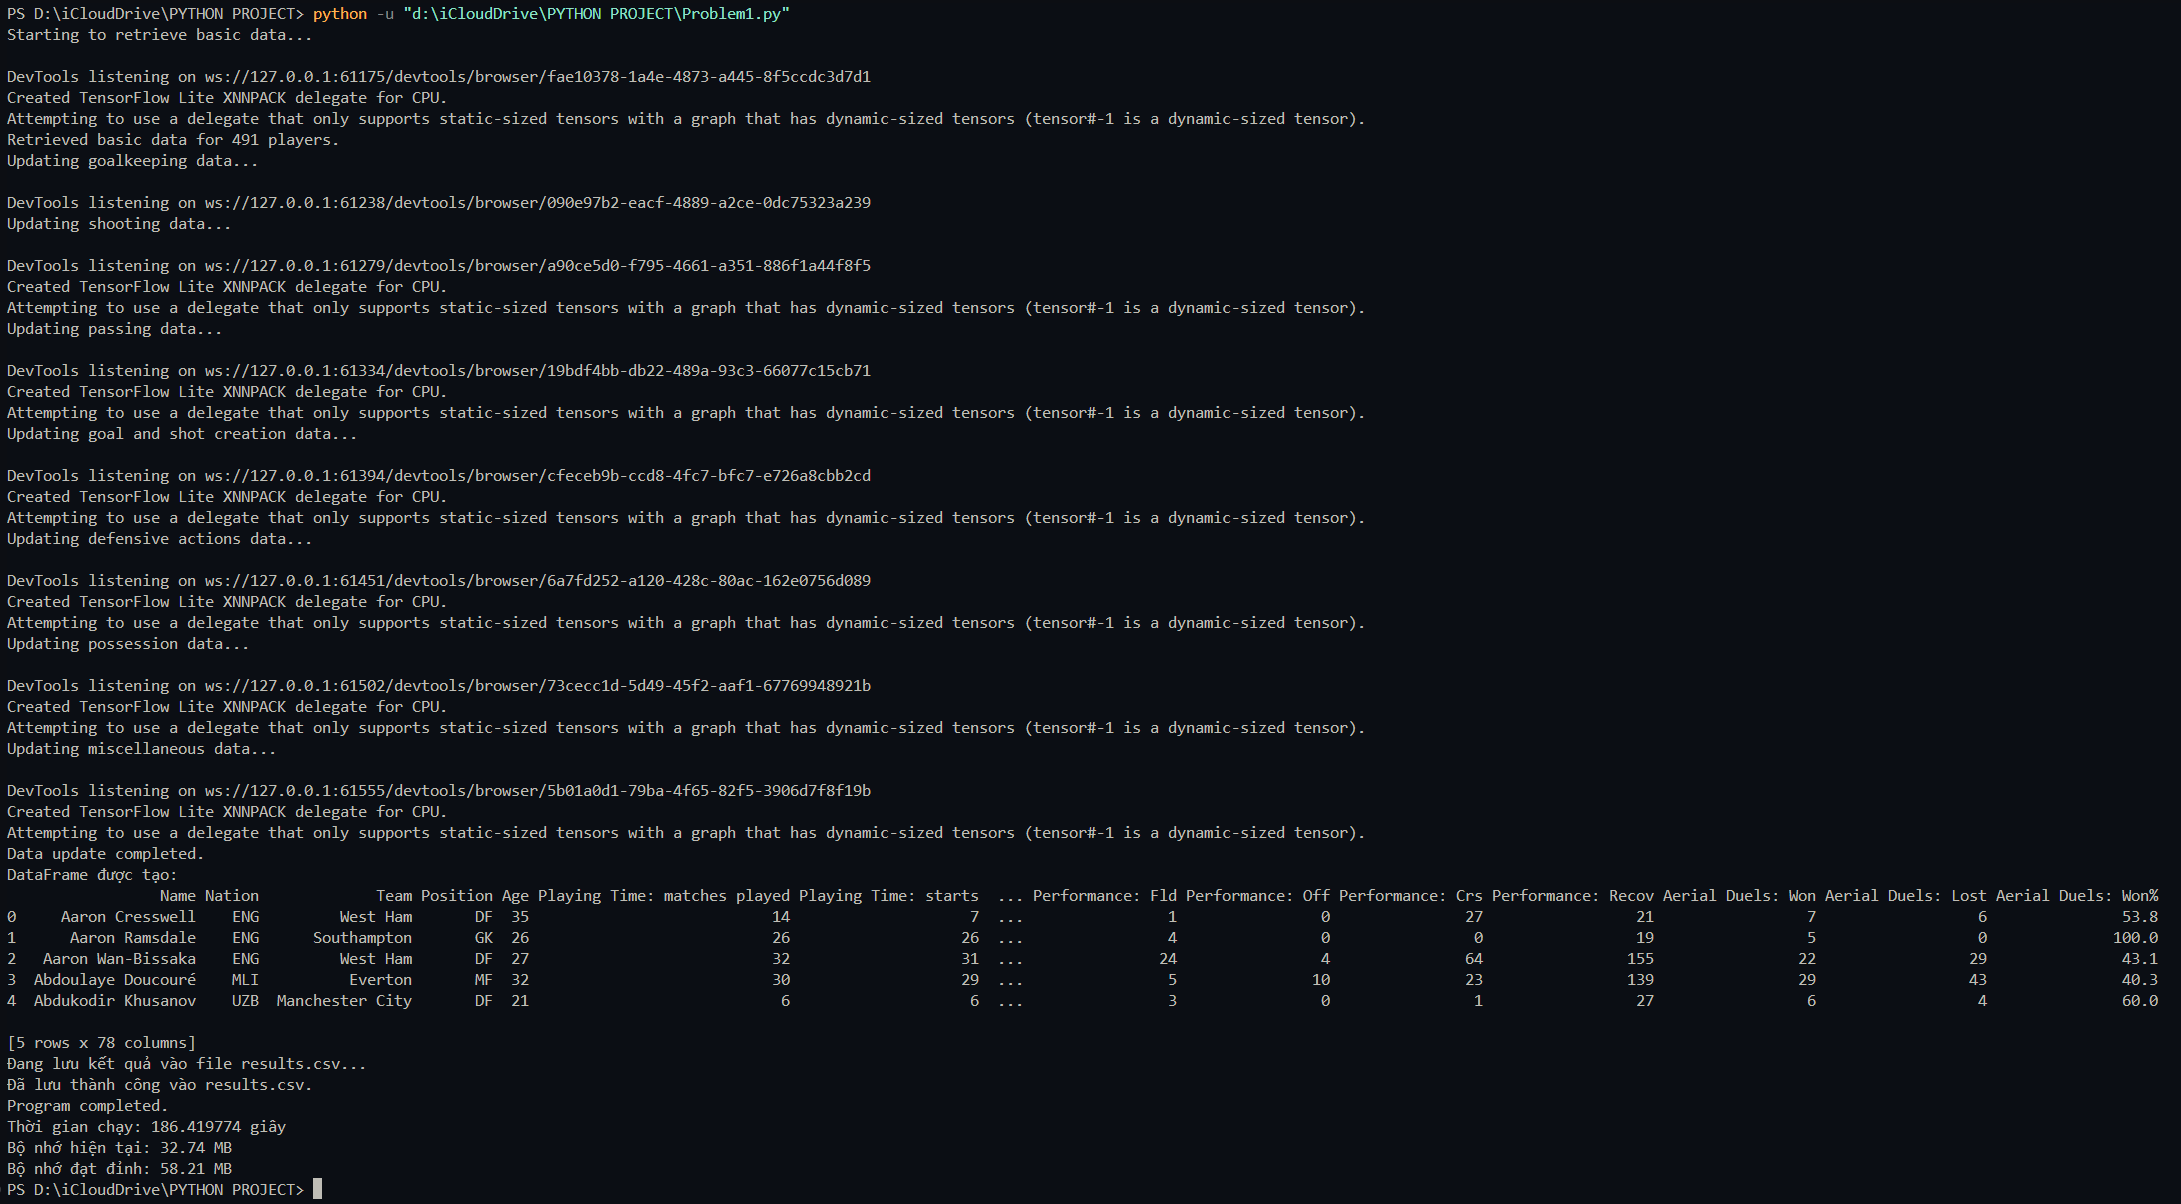
\includegraphics[width=\textwidth]{Terminal.png}
    \caption{Terminal sau khi chạy chương trình Problem1.py}
    \label{fig:terminal}
\end{figure}
Thu thập Dữ liệu: Script bắt đầu bằng việc thông báo "Starting to retrieve team data..." (Bắt đầu truy xuất dữ liệu đội) và sau đó là "Retrieved basic data for 491 players." (Đã truy xuất dữ liệu cơ bản cho 419 cầu thủ). Tiếp theo, nó cập nhật các loại dữ liệu khác nhau như dữ liệu hiệu suất, dữ liệu đội hình xuất phát, dữ liệu tạo cơ hội ghi bàn và sút bóng, dữ liệu hành động phòng ngự, và dữ liệu kiểm soát bóng.
\\
Kết nối DevTools: Các dòng "DevTools listening on ws://127.0.0.1:..." lặp lại nhiều lần. Điều này thường xuất hiện khi một công cụ tự động hóa trình duyệt (Selenium) được sử dụng, có thể là để lấy dữ liệu từ các trang web.\\
Hiển thị Dữ liệu Dạng Bảng: Sau khi cập nhật dữ liệu xong ("Data update completed."), script hiển thị một phần của bảng dữ liệu. Bảng hiển thị 5 dòng đầu tiên và có tổng cộng 78 cột.\\
Lưu và Xếp hạng Kết quả: Script thông báo "All data written to the file results.csv." (Tất cả dữ liệu đã được ghi vào tệp results.csv) và sau đó "Attempting to rank the results.csv." (Đang cố gắng xếp hạng tệp results.csv).\\
Hoàn thành và Thời gian Thực thi: Cuối cùng, script báo "Process complete." (Quá trình hoàn tất) và cho biết thời gian thực thi là khoảng 186.419472 giây; Bộ nhớ tối đa sử dụng: 32.74 MB; Bộ nhớ đạt đỉnh: 58.21 MB.\\\\
\begin{figure}[h]
    \centering
    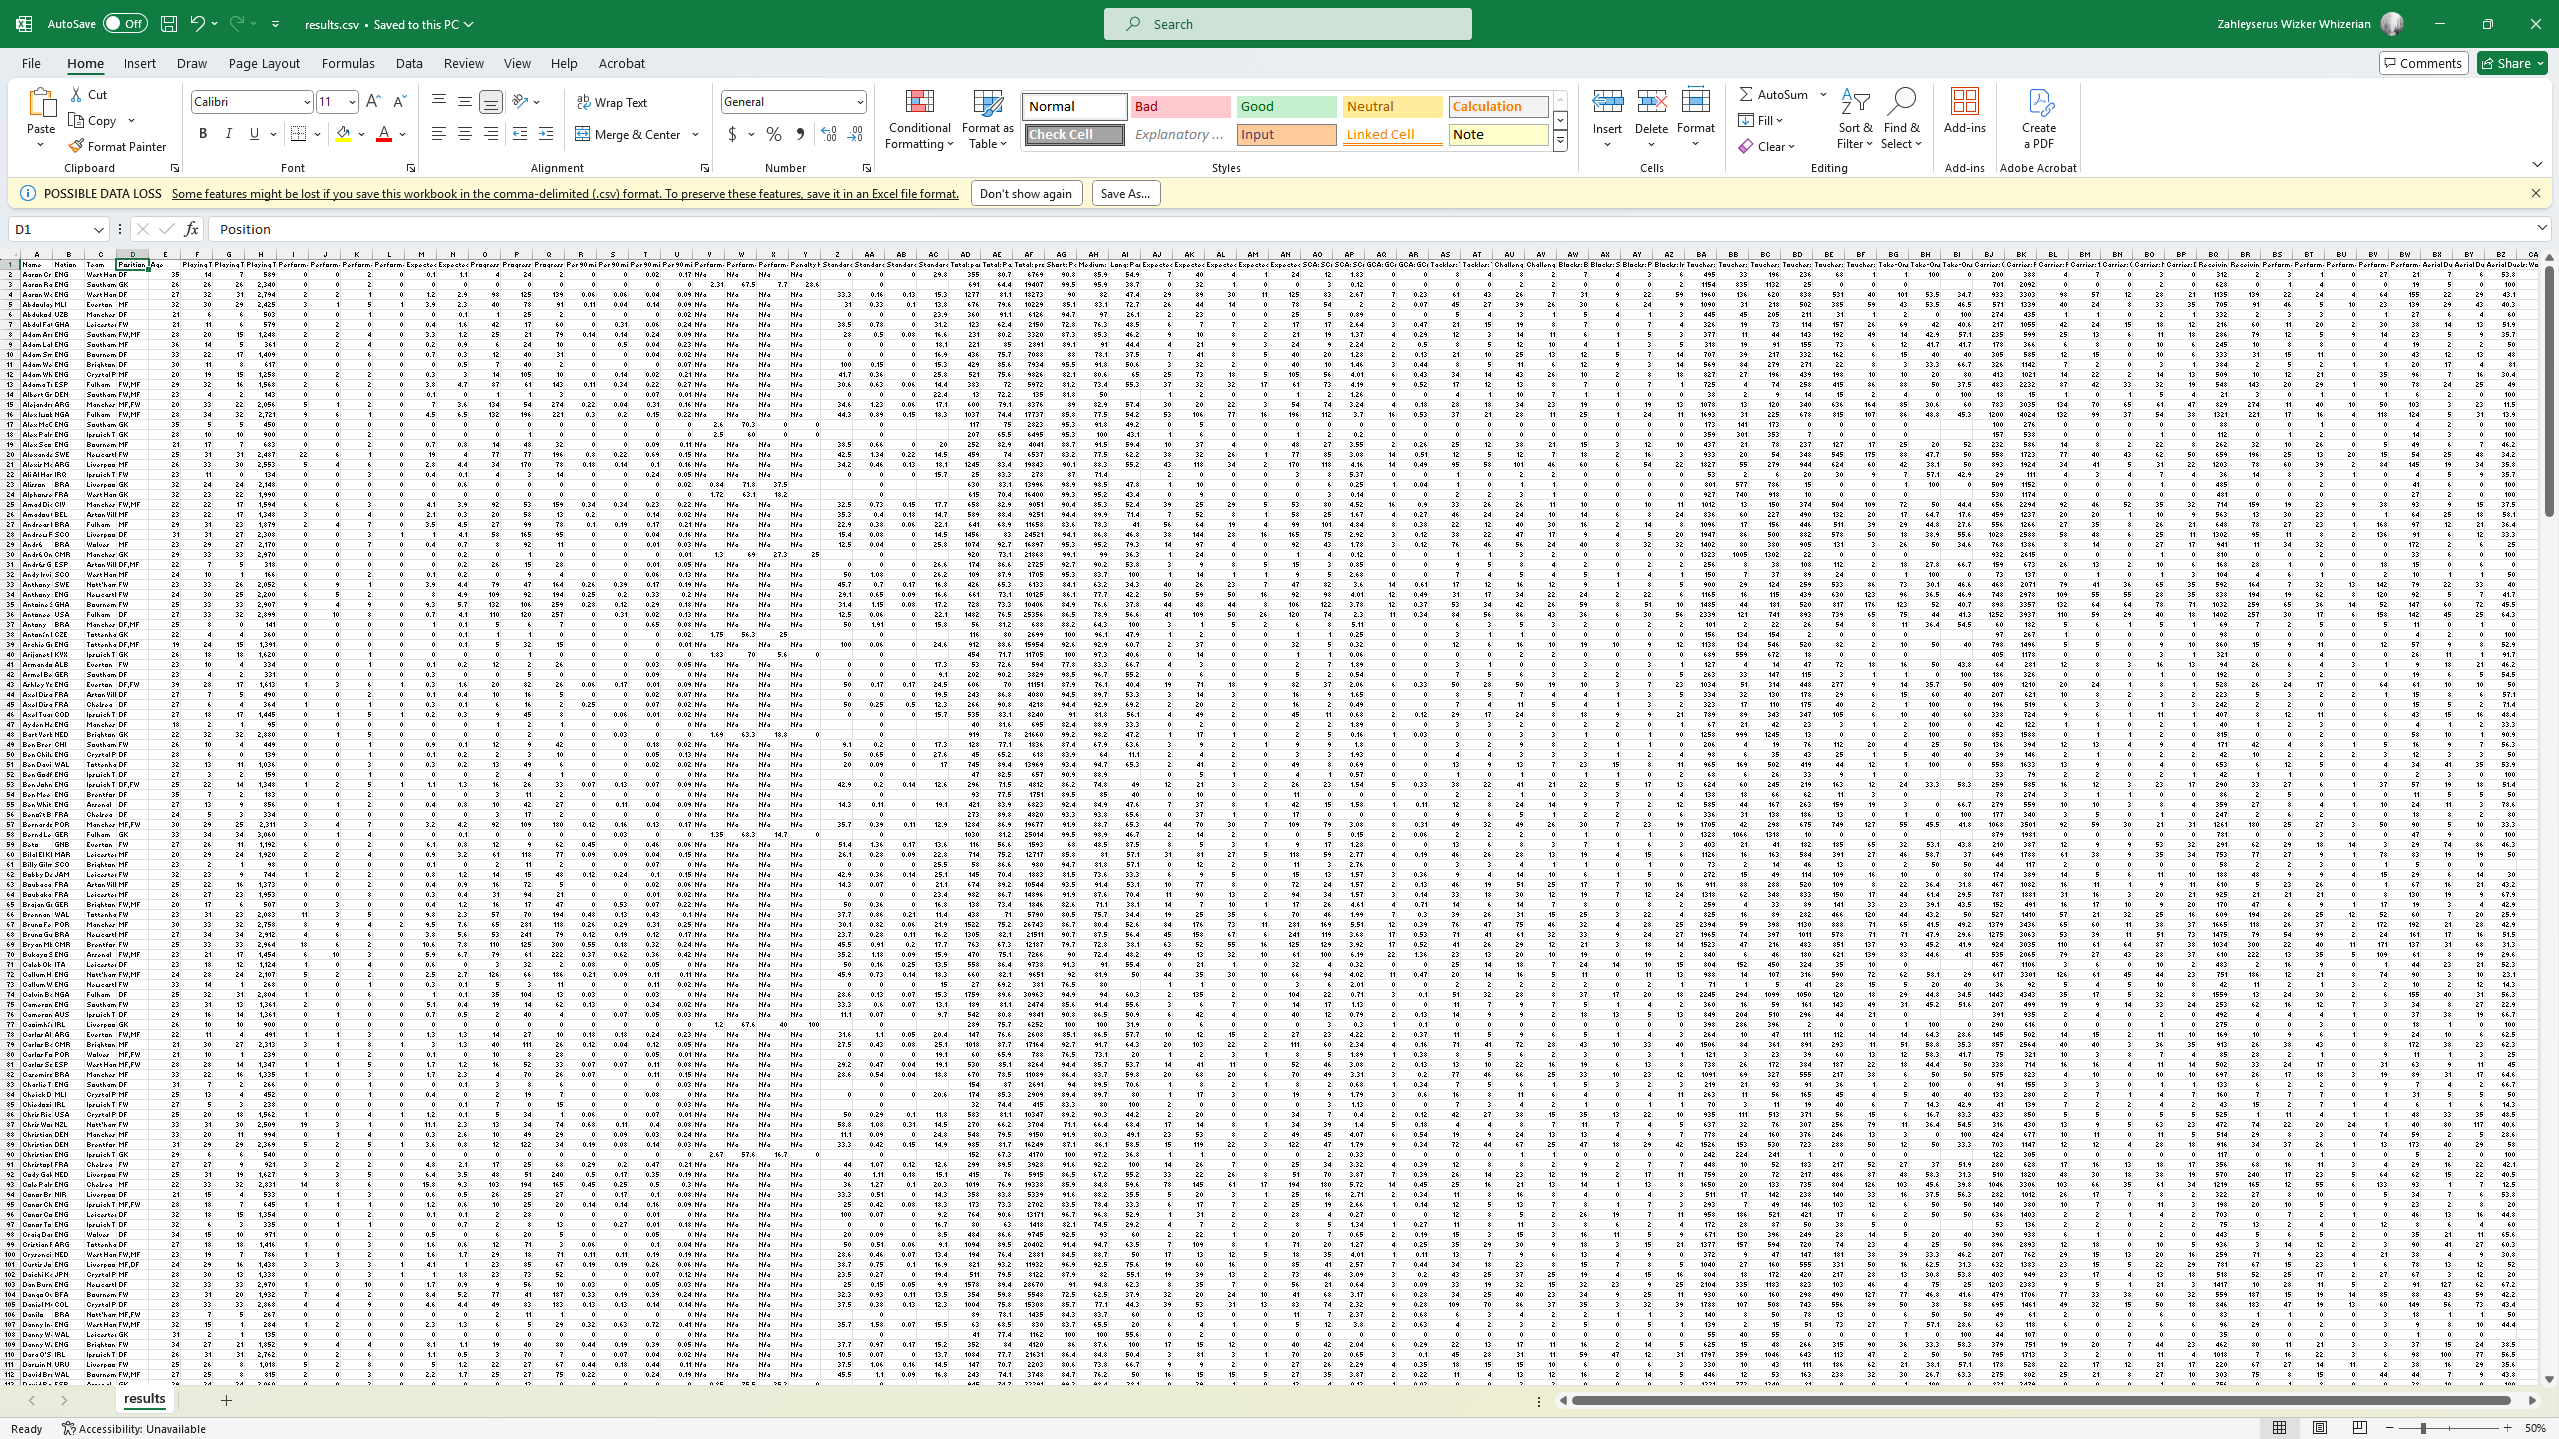
\includegraphics[width=\textwidth]{results_csv.png}
    \caption{File results.csv}
    \label{fig:terminal}
\end{figure}
Tệp dữ liệu results.csv tập hợp thông tin thống kê chi tiết của 491 vận động viên bóng đá chuyên nghiệp, với mỗi đối tượng được mô tả thông qua 78 biến số định lượng và định tính. Các trường dữ liệu bao gồm thông tin cá nhân (họ tên, quốc tịch, câu lạc bộ chủ quản, vị trí thi đấu, độ tuổi), thông tin về thời lượng thi đấu (số trận ra sân, số trận đá chính, tổng số phút thi đấu), thành tích thi đấu (số bàn thắng, số đường kiến tạo, số thẻ phạt), cùng các chỉ số dự đoán hiệu suất (Expected Goals - xG, Expected Assisted Goals - xAG). Ngoài ra, bộ dữ liệu còn cung cấp các chỉ số liên quan đến kỹ năng kiểm soát bóng, chuyền bóng, rê dắt, phòng ngự, khả năng tiến bộ bóng (progression), hiệu suất trung bình chuẩn hóa trên 90 phút thi đấu, cũng như hiệu quả tranh chấp tay đôi trên không.
\subsection{Đánh giá:}
Chương trình trong tập tin Problem1.py triển khai quy trình thu thập, tổng hợp và xuất dữ liệu thống kê chi tiết của các cầu thủ Premier League thông qua kỹ thuật web scraping, kết hợp Selenium và BeautifulSoup. Dữ liệu được trích xuất từ nhiều bảng thống kê chuyên biệt trên fbref.com, bao gồm các chỉ số tiêu chuẩn, chỉ số thủ môn, khả năng dứt điểm, chuyền bóng, kiểm soát bóng, phòng ngự và các chỉ số hỗn hợp khác. Mỗi cầu thủ được biểu diễn dưới dạng một từ điển với khóa định danh duy nhất (kết hợp tên và câu lạc bộ), đảm bảo tính toàn vẹn dữ liệu trong quá trình cập nhật từ nhiều nguồn. Sau khi thu thập đầy đủ, chương trình xây dựng một DataFrame gồm 78 thuộc tính và xuất kết quả ra tệp CSV định dạng chuẩn, phục vụ cho phân tích dữ liệu thống kê sâu hơn.

Về mặt thời gian thực thi, chương trình hoàn thành toàn bộ quy trình trong khoảng 186.4 giây, thể hiện khả năng thu thập dữ liệu chi tiết và chính xác nhưng hiệu suất còn thấp. Nguyên nhân chủ yếu đến từ việc khởi tạo nhiều phiên trình duyệt Chrome độc lập cho từng loại bảng dữ liệu, gây ra chi phí khởi động, tải trang và đóng trình duyệt lặp lại nhiều lần. Về mặt sử dụng bộ nhớ, chương trình hoạt động hiệu quả, chỉ sử dụng tối đa khoảng 32.74 MB bộ nhớ RAM trong suốt quá trình thu thập và xử lý, cho thấy sự tiết kiệm tài nguyên bộ nhớ nhờ vào việc lưu trữ dữ liệu theo cấu trúc đơn giản và xử lý tuần tự.

Tóm lại, chương trình đạt độ chính xác cao và tổ chức dữ liệu hệ thống tốt, song tồn tại nhược điểm rõ rệt về thời gian thực thi do thiết kế chưa tối ưu hóa quy trình truy cập web, trong khi ưu điểm nổi bật là mức sử dụng bộ nhớ thấp, phù hợp với các hệ thống hạn chế về tài nguyên.
}
\clearpage
\chapter{VẤN ĐỀ II}
{
\section{Yêu cầu}
\begin{itemize}
	\item Identify the top 3 players with the highest and lowest scores for each statistic. Save result to a file named \texttt{top\_3.txt}.
	\item Find the median for each statistic. Calculate the mean and standard deviation for each statistic across all players and for each team. Save the results to a file named 'results2.csv' with the following format:
	\begin{table}[h]
		\centering
		\begin{tabular}{|c|c|c|c|c|c|}
		\hline
		 &  & Median of Attribute 1 & Mean of Attribute 1 & Std of Attribute 1 & \ldots \\ \hline
		0 & all &  &  &  &  \\ \hline
		1 & Team 1 &  &  &  &  \\ \hline
		\vdots & \vdots &  &  &  &  \\ \hline
		n & Team n &  &  &  &  \\ \hline
		\end{tabular}
		\caption{Statistics per team}
	\end{table}
	\item Plot a histogram showing the distribution of each statistic for all players in the league and each team.
	\item Identify the team with the highest scores for each statistic. Based on your analysis, which team do you think is performing the best in the 2024-2025 Premier League season?
\end{itemize}
\section{Các bước tiến hành}
\begin{enumerate}
	\item Thực hiện phân tích dữ liệu thống kê của các cầu thủ bóng đá từ file CSV đầu vào (results.csv). Đầu tiên, đọc dữ liệu, xử lý các cột số liệu và phân chia thành nhóm thông tin định tính và định lượng.
	\item Sau đó, chương trình tiến hành tìm kiếm Top 3 cầu thủ có chỉ số cao nhất và thấp nhất cho từng loại thống kê. Đưa kết quả ra file top3.txt như yêu cầu.
	\item Tính toán các thống kê tổng hợp như trung bình, trung vị và độ lệch chuẩn cho toàn bộ giải đấu cũng như cho từng đội bóng riêng biệt. Các kết quả này được lưu lại thành file results2.csv như yêu cầu đề bài.
	\item Trực quan hóa dữ liệu bằng cách vẽ các biểu đồ phân phối cho các chỉ số, bao gồm cả biểu đồ tổng thể toàn giải và biểu đồ chi tiết cho từng đội bóng. Các biểu đồ này được lưu dưới dạng hình ảnh.
	\item Xác định đội bóng mạnh nhất dựa trên việc so sánh trung bình các chỉ số, và tổng hợp đội có nhiều chỉ số tốt nhất thành "Best Overall Team". Kết quả này cũng được ghi lại.
\end{enumerate}
\section{Code thực tế và mô tả chi tiết}
\subsection{Hàm chính}
\lstset{
    language=Python,
    basicstyle=\ttfamily\scriptsize,
    keywordstyle=\color[rgb]{0.878, 0.467, 0.0}, % màu xanh đậm cho keyword
    commentstyle=\color[rgb]{0.5,0.5,0.5}, % màu xám cho comment
    stringstyle=\color[rgb]{0, 0.4, 0},
    identifierstyle=\color[rgb]{0.0, 0.298, 0.380},    % bình thường cho biến
    numbers=left,
    numberstyle=\tiny\color[rgb]{0.5,0.5,0.5},
    numbersep=5pt,
    showstringspaces=false,
    breaklines=true,
    tabsize=2
}
\begin{lstlisting}
def Problem_2():
    df, stats_cols, non_numeric_cols = read_data()
    # 1. Find top 3 highest and lowest for each statistic
    Find_Top_3(df, stats_cols)
    # 2. Calculate Median, Mean, Std for each statistic
    Calculate_For_Each_Statistic(df, stats_cols)
    # 3. Plotting
    Plotting(df)
    # 4. Identify the best team for each statistic
    Best_Team_Summary(df, stats_cols)
\end{lstlisting}
\textbf{Các thao tác được thực hiện theo đúng trình tự đã mô tả ở phần các bước tiến hành:}\\

\textbf* {Hàm read\_data():} Nhập dữ liệu đầu vào:
\begin{itemize}
	\item Nhập dữ liệu đầu vào từ file results.csv đã lưu ở Vấn đề 1 (thay vì đi lấy dữ liệu 1 lần nữa).
	\item Trả về DataFrame, Cột thống kê, cột không chứa số (dữ liệu phân tích). 
\end{itemize}

\textbf* {Hàm Find\_Top\_3(df, stats\_cols)}
\begin{itemize}
	\item Nạp dữ liệu vào là DataFrame và các cột thống kê (Kết quả của fuction read\_data()).
	\item Thực hiện việc tìm top 3 (cao nhất và thấp nhất của mỗi chỉ số).
	\item Xuất dữ liệu ra file top\_3.txt theo yêu cầu.
\end{itemize}

\textbf* {Calculate\_For\_Each\_Statistic(df, stats\_cols)}
\begin{itemize}
	\item Nạp dữ liệu vào là DataFrame và các cột thống kê (Kết quả của fuction read\_data()).
	\item Tiến hành thực hiện các bước để đưa các giá các giá trị ở mỗi team (trung bình, độ lệch) cho tất cả các trường.
	\item Đưa về đúng các trường như yêu cầu rồi cố định vào trong DataFrame.
	\item Xuất dữ liệu ra file 'results2.csv' như yêu cầu.
\end{itemize}

\textbf* {Hàm Plotting(df)}
\begin{itemize}
	\item Nạp dữ liệu vào là DataFrame (Kết quả của fuction read\_data())
	\item Tiến hành thực hiện các bước vẽ đồ thị tổng hợp. Vẽ theo đúng 3 chỉ số tấn công, 3 chỉ số phòng thủ. Đưa kết quả ra.
	\item Lần lượt vẽ đồ thị theo từng chỉ số, gói dữ liệu về theo từng team để tạo đồ thị (mỗi team 1 đồ thị). Đưa dữ liệu ra.
\end{itemize}

\textbf* {Hàm Best\_Team\_Summary(df, stats\_cols)}
\begin{itemize}
	\item Nạp dữ liệu vào là DataFrame và các cột thống kê (Kết quả của fuction read\_data()).
	\item Xử lý dữ liệu, tìm ra team có giá trị lớn nhất theo từng chỉ số.
	\item Đếm số lượng chỉ số dẫn đầu của mỗi team để tìm ra team có phong độ tốt nhất, từ đó đưa ra dự đoán.
\end{itemize}

\subsection{Chi tiết các thao tác}
\textbf* {Thao tác read\_data() (Đọc dữ liệu vào):}
\lstset{
    language=Python,
    basicstyle=\ttfamily\scriptsize,
    keywordstyle=\color[rgb]{0.878, 0.467, 0.0}, % màu xanh đậm cho keyword
    commentstyle=\color[rgb]{0.5,0.5,0.5}, % màu xám cho comment
    stringstyle=\color[rgb]{0, 0.4, 0},
    identifierstyle=\color[rgb]{0.0, 0.298, 0.380},    % bình thường cho biến
    numbers=left,
    numberstyle=\tiny\color[rgb]{0.5,0.5,0.5},
    numbersep=5pt,
    showstringspaces=false,
    breaklines=true,
    tabsize=2
}
\begin{lstlisting}
def read_data():
    # Load the data
    df = pd.read_csv(results.csv)

    # Columns that are not statistics
    non_numeric_cols = ['Name', 'Nation', 'Team', 'Position', 'Age']
    stats_cols = [col for col in df.columns if col not in non_numeric_cols]

    # Clean numeric columns (remove commas and convert to numbers)
    for col in stats_cols:
        df[col] = df[col].astype(str).str.replace(',', '', regex=False)
        df[col] = pd.to_numeric(df[col], errors='coerce')

    return df, stats_cols, non_numeric_cols
\end{lstlisting}

Ở thao tác này, trước hết phải lấy dữ liệu từ file: results.csv, tạo một DataFrame mới chứa dữ liệu này [dòng 3]; Xử lý, tách những dữ liệu cần thống kê (về list) và không cần thống kê [dòng 6, 7]. Sau khi đã cơ bản lấy được dữ liệu tiếp tục đi xử lý một vài vùng dữ liệu như số có dấu ',', chuyển thành chữ số [dòng 10 - 12]. Trả về kết quả là những DataFrame, list vừa xử lý.\\

\textbf* {Thao tác Find\_Top\_3(df, stats\_cols) (Tìm top 3 cầu thủ đứng đầu và cuối ở mỗi chỉ số)}
\lstset{
    language=Python,
    basicstyle=\ttfamily\scriptsize,
    keywordstyle=\color[rgb]{0.878, 0.467, 0.0}, % màu xanh đậm cho keyword
    commentstyle=\color[rgb]{0.5,0.5,0.5}, % màu xám cho comment
    stringstyle=\color[rgb]{0, 0.4, 0},
    identifierstyle=\color[rgb]{0.0, 0.298, 0.380},    % bình thường cho biến
    numbers=left,
    numberstyle=\tiny\color[rgb]{0.5,0.5,0.5},
    numbersep=5pt,
    showstringspaces=false,
    breaklines=true,
    tabsize=2
}
\begin{lstlisting}
def Find_Top_3(df, stats_cols):
    top3_results = []

    for col in stats_cols:
        if df[col].dropna().empty:
            continue  # Skip empty columns
        
        # Top 3 highest
        top_high = df[['Name', 'Team', col]].sort_values(by=col, ascending=False).head(3)
        
        # Top 3 lowest
        top_low = df[['Name', 'Team', col]].sort_values(by=col, ascending=True).head(3)
        
        section = f"=== {col} ===\n"
        section += "Top 3 Highest:\n"
        for idx, row in top_high.iterrows():
            section += f"  {row['Name']} ({row['Team']}): {row[col]}\n"
        
        section += "Top 3 Lowest:\n"
        for idx, row in top_low.iterrows():
            section += f"  {row['Name']} ({row['Team']}): {row[col]}\n"
        
        section += "\n"
        top3_results.append(section)

    # Save to top_3.txt
    with open('top_3.txt', 'w', encoding='utf-8') as f:
        f.write("\n".join(top3_results))

    print("top_3.txt saved!")
\end{lstlisting}
Đầu tiên, khởi tạo một list dùng để chứa các dữ liệu đầu ra [dòng 2]. Bắt đầu chạy từng cột trong bảng những giá trị thống kê. Bở qua những cột trống (Tránh nhiễu dữ liệu nếu có) [dòng 5, 6]. Tạo một DataFrame mới lưu top 3 của chỉ số (Cao nhất và thấp nhất) [dòng 9, 12].\\
Dòng 14 đến 23 là các thao tác tạo dữ liệu để đưa vào ra (viết các mô tả để dễ dọc file đầu ra). Ở thao tác này lấy tên cầu thủ, tên team, và giá trị ở cột đang xét.\\
Sau khi viết xong đưa vào list đã tạo ở đầu. Tiếp tục lặp tới hết cột của bảng.\\
Sau khi lấy hết kết quả tiến hành ghi kết quả vào file top\_3.txt như yêu cầu [dòng 27 - 29].\\

\textbf* {Thao tác Calculate\_For\_Each\_Statistic(df, stats\_cols) (Tạo bảng thống kê các trung bình, trung vị, độ lệch của các team)}
\lstset{
    language=Python,
    basicstyle=\ttfamily\scriptsize,
    keywordstyle=\color[rgb]{0.878, 0.467, 0.0}, % màu xanh đậm cho keyword
    commentstyle=\color[rgb]{0.5,0.5,0.5}, % màu xám cho comment
    stringstyle=\color[rgb]{0, 0.4, 0},
    identifierstyle=\color[rgb]{0.0, 0.298, 0.380},    % bình thường cho biến
    numbers=left,
    numberstyle=\tiny\color[rgb]{0.5,0.5,0.5},
    numbersep=5pt,
    showstringspaces=false,
    breaklines=true,
    tabsize=2
}
\begin{lstlisting}
def save_df_to_file(name, res):
    results_df.to_csv(name, index=False, encoding='utf-8-sig')

def Calculate_For_Each_Statistic(df, stats_cols):
    # Group by Team + one overall ("all")
    grouped = df.groupby('Team')
    summary_rows = []

    # First row: "all" players
    summary_all = {'Team': 'all'}
    for col in stats_cols:
        summary_all[f'Median of {col}'] = df[col].median()
        summary_all[f'Mean of {col}'] = df[col].mean()
        summary_all[f'Std of {col}'] = df[col].std()
    summary_rows.append(summary_all)

    # Each team's stats
    for team, team_df in grouped:
        summary_team = {'Team': team}
        for col in stats_cols:
            summary_team[f'Median of {col}'] = team_df[col].median()
            summary_team[f'Mean of {col}'] = team_df[col].mean()
            summary_team[f'Std of {col}'] = team_df[col].std()
        summary_rows.append(summary_team)

    # Save to results2.csv
    save_df_to_file('results2.csv', summary_rows)
    print("results2.csv saved!")
\end{lstlisting}

Khởi tạo các thành phần cần thiết để xử lý dữ liệu: Tạo DataFrame gộp lại bởi các team [dòng 8]; Tạo một list lưu trữ các giá trị theo từng dòng [dòng 9].\\
Xử lý các giá trị ở dòng đầu (all) lặp trên từng cột của bảng thống kê tự đó đưa ra 3 giá trị như yêu cầu [Dòng 12 - 17].\\
Xử lý các dữ liệu của từng dòng team. Thực hiện vòng lặp để tìm từng theo từng team. Tiếp tục tạo vòng lặp theo từng trường dữ liệu đưa ra 3 chỉ số theo yêu cầu của từng trường và đưa vào list lưu kết quả. Lặp cho đến khi hết team [Dòng 20 - 26].\\
Đưa ra dữ liệu vào file results2.csv thông qua hàm save\_df\_to\_file(name, res).\\

\textbf* {Thao tác Plotting(df) (Tạo biểu đồ)}
\lstset{
    language=Python,
    basicstyle=\ttfamily\scriptsize,
    keywordstyle=\color[rgb]{0.878, 0.467, 0.0}, % màu xanh đậm cho keyword
    commentstyle=\color[rgb]{0.5,0.5,0.5}, % màu xám cho comment
    stringstyle=\color[rgb]{0, 0.4, 0},
    identifierstyle=\color[rgb]{0.0, 0.298, 0.380},    % bình thường cho biến
    numbers=left,
    numberstyle=\tiny\color[rgb]{0.5,0.5,0.5},
    numbersep=5pt,
    showstringspaces=false,
    breaklines=true,
    tabsize=2
}
\begin{lstlisting}
def Plotting(df):
    # --- Setting up ---
    attack_indexes = [
        'Performance: goals',  
        'Performance: assists', 
        'Expected: expected goals (xG)'
    ]

    defense_indexes = [
        'Tackles: Tkl', 
        'Challenges: Att', 
        'Blocks: Blocks'   
    ]

    team_column_name = 'Team'
    max_teams_per_row_facet = 4 # How many team plots per row in FacetGrid
    all_indexes = attack_indexes + defense_indexes
    valid_indexes = []

    for col in all_indexes:
        if col in df.columns:
            df[col] = pd.to_numeric(df[col], errors='coerce')
            if not df[col].isnull().all() and pd.api.types.is_numeric_dtype(df[col]):
                valid_indexes.append(col)

    # --- Plotting ---
    # 1. Histograms for the Entire League
    Histograms_Entire_League(df, valid_indexes)
    
    # 2. Histograms per Team (using FacetGrid)
    Histograms_per_Team(df, team_column_name, valid_indexes, max_teams_per_row_facet)
    
    print("\n--- Plotting Complete ---")
\end{lstlisting}
Ở function này bao gồm 2 thao tác chính: Chuẩn bị (được code toàn bộ trong function); Vẽ biểu đồ (ở trong 2 function phụ được gọi). Đi sâu và chi tiết:\\
\textbf{Setting Up:}\\
Khởi tạo các giá trị sẽ tiến hành lấy dữ liệu để vẽ biểu đồ [Dòng 3 - 15] (Bao gồm 6 thuộc tính: 3 thuộc tính về tấn công, 3 thuộc tính về phòng thủ). Tiếp tục khởi tạo một số giá trị cần thiết nhằm phục vụ cho quá trình xử lý dữ liệu và vẽ biểu đồ [dòng 15 - 18]. Thực hiện vòng lặp nhằm đưa dữ liệu về dạng số đồng thời loại bỏ những thuộc tính không thể thống kê (Đảm bảo không có lỗi khi chạy).

\textbf{Plotting:} Thao tác được thực hiện thông qua 2 chương trình con:\\
\textbf* {Histograms\_Entire\_League(df, valid\_indexes) Đồ thị tổng hợp: }
\begin{lstlisting}
def Histograms_Entire_League(df, valid_indexes):
    print("\n--- Plotting Overall League Distributions ---")
    num_valid_indexes = len(valid_indexes)
    # Calculate grid size for overall plots (e.g., 2 columns)
    ncols_overall = 2
    nrows_overall = (num_valid_indexes + ncols_overall - 1) // ncols_overall

    plt.figure(figsize=(12, 5 * nrows_overall))
    plt.suptitle('Overall League Distribution of Player Indexes', fontsize=16, y=1.02) # Add space with y

    for i, index_col in enumerate(valid_indexes):
        plt.subplot(nrows_overall, ncols_overall, i + 1)
        # Filter out NaN values for plotting if you didn't fill them earlier
        data_to_plot = df[index_col].dropna()
        if not data_to_plot.empty:
            sns.histplot(data_to_plot, kde=True, bins=20)
            plt.title(f'Distribution of {index_col}')
            plt.xlabel(index_col)
            plt.ylabel('Frequency')
        else:
            plt.title(f'{index_col}\n(No valid data to plot)')

    plt.tight_layout(rect=[0, 0, 1, 0.98]) # Adjust layout to prevent overlap with suptitle
    plt.savefig(os.path.join('P2_RES', 'Overall_League_Distribution_of_Player_Indexes.png'))
    print("\n--- Done Plotting Overall League Distributions ---")
\end{lstlisting}
Trước tiên function lấy vào cũng như khởi tạo một số giá trị để phục vụ việc bố trí. (đưa vào số đồ thị [dòng 3]; khởi tạo các thông số để bố trí hình dọc theo 2 biểu đồ 1 dòng [dòng 5, 6]). Dòng 8 tiến hành tạo khích thước cho biểu đồ mặc định là 12 x 5*(số lượng dòng biểu đồ). Tạo tên cho ảnh ở dòng 9.\\
Tiến hành lặp để vẽ biểu đồ theo từng loại chỉ số được đưa vào. Dòng 12 nhằm đưa biểu đồ về đúng vị trí đã bố trí trước đó. Dòng 14 nhằm lọc bỏ những giá trị không hợp lệ, ví dụ: \texttt{'N/a'}. Nếu có giá trị thì tiến hành vẽ biểu đồ, nếu không thì tạo ô trống với định dạng tên như ở dòng 21.

Trong khi tạo biểu đồ, ta dùng lệnh:
sns.histplot(data\_to\_plot, kde=True, bins=20)
để vẽ biểu đồ histogram (biểu đồ tần suất) của dữ liệu trong \texttt{data\_to\_plot}.

\begin{itemize}
    \item \texttt{data\_to\_plot}: là dữ liệu bạn muốn vẽ histogram, có thể là một danh sách, mảng NumPy, Series Pandas, v.v.
    \item \texttt{bins=20}: chia dữ liệu thành 20 khoảng (bins) để vẽ histogram. Mỗi cột trong biểu đồ đại diện cho số lượng phần tử nằm trong một khoảng nhất định.
    \item \texttt{kde=True}: vẽ thêm đường mật độ kernel (KDE) – một đường cong trơn ước lượng phân phối xác suất của dữ liệu, giúp bạn nhìn rõ dạng phân phối (ví dụ: chuẩn, lệch trái, lệch phải, v.v.).
\end{itemize}
Sau khi lặp xong hết các chỉ số, ta cố định layout và lưu ảnh [dòng 23, 24].\\
\textbf* { Histograms\_per\_Team(df, team\_column\_name, valid\_indexes, max\_teams\_per\_row\_facet)) Đồ thị theo từng chỉ số của mỗi team: }
\begin{lstlisting}
def Histograms_per_Team(df, team_column_name, valid_indexes, max_teams_per_row_facet):
    print("\n--- Plotting Per-Team Distributions ---")

    # Check number of unique teams to avoid overly large grids
    unique_teams = df[team_column_name].nunique()
    print(f"Found {unique_teams} unique teams.")
    if unique_teams > 50: # Add a threshold to prevent overwhelming plots
        print("Warning: High number of teams detected. FacetGrid might be very large.")
        # Optional: Add logic here to maybe plot only a subset of teams or ask user

    for index_col in valid_indexes:
        print(f"Generating FacetGrid for: {index_col}")

        # Filter out NaNs for this specific index and the team column before creating the grid
        facet_data = df[[index_col, team_column_name]].dropna()

        if facet_data.empty or facet_data[index_col].isnull().all():
            print(f"  Skipping {index_col} - No valid data after dropping NaNs.")
            continue

        # Create the FacetGrid
        g = sns.FacetGrid(
            facet_data,
            col=team_column_name,
            col_wrap=min(max_teams_per_row_facet, unique_teams), # Don't wrap more than teams exist
            sharex=True, # Keep x-axis consistent for comparison
            sharey=False, # Allow y-axis (frequency) to vary per team
            height=3,    # Adjust height of each subplot
            aspect=1.2   # Adjust aspect ratio of each subplot
        )

        # Map the histogram plot onto the grid
        g.map(sns.histplot, index_col, kde=True, bins=15) # Use fewer bins for smaller plots

        # Add titles and adjust layout
        g.set_titles("Team: {col_name}")
        g.fig.suptitle(f'Distribution of {index_col.split} by Team', fontsize=14, y=1.03) # Add overall title slightly above
        g.fig.tight_layout(rect=[0, 0, 1, 0.97]) # Adjust layout
        name = (index_col.replace(' ', '_')).replace(':', '')
        plt.savefig(os.path.join('P2_RES','Distribution_of_'+name+'_by_Team.png'))
    print("\n--- Done Plotting Per-Team Distributions ---")
\end{lstlisting}
\begin{itemize}
    \item Ban đầu, hàm in thông báo bắt đầu quá trình vẽ biểu đồ và xác định số lượng đội bóng khác nhau trong dữ liệu đầu vào. Nếu số lượng đội quá lớn, chương trình sẽ đưa ra cảnh báo về nguy cơ quá tải biểu đồ (dòng 5–8).
    \item Sau đó, hàm lặp qua từng chỉ số trong danh sách \texttt{valid\_indexes}. Với mỗi chỉ số, dữ liệu được lọc để chỉ giữ lại những giá trị hợp lệ tương ứng với chỉ số và tên đội (dòng 11–12). Nếu toàn bộ dữ liệu của chỉ số đó là thiếu (\texttt{NaN}), chỉ số sẽ bị bỏ qua (dòng 17–18).
    \item Đối với các chỉ số có dữ liệu hợp lệ, hàm tạo một lưới biểu đồ (\texttt{FacetGrid}) trong đó mỗi ô biểu diễn phân phối của chỉ số theo từng đội bóng. Lưới được điều chỉnh với chiều cao, tỉ lệ, và số cột phù hợp, đồng thời giữ cố định trục hoành giữa các biểu đồ để thuận tiện cho việc so sánh (dòng 22–30).
    \item Biểu đồ histogram với 15 khoảng (\texttt{bins}) cùng với đường mật độ KDE được ánh xạ lên từng ô trong lưới (dòng 33). Mỗi ô có tiêu đề phụ hiển thị tên đội, đồng thời tiêu đề chung cho toàn bộ lưới được thêm phía trên cùng. Hàm sử dụng \texttt{tight\_layout()} để căn chỉnh bố cục tránh chồng lấn (dòng 36–38).
    \item Cuối cùng, biểu đồ được lưu vào thư mục \texttt{P2\_RES} với tên tệp động dựa trên chỉ số đang xử lý (dòng 40), và thông báo kết thúc quá trình vẽ biểu đồ được in ra (dòng 41).
\end{itemize}
\textbf* {Thao tác Best\_Team\_Summary(df, stats\_cols): Tìm ra team tốt nhất ở mỗi chỉ số và dự đoán team có thành tích tốt nhất}
\lstset{
    language=Python,
    basicstyle=\ttfamily\scriptsize,
    keywordstyle=\color[rgb]{0.878, 0.467, 0.0}, % màu xanh đậm cho keyword
    commentstyle=\color[rgb]{0.5,0.5,0.5}, % màu xám cho comment
    stringstyle=\color[rgb]{0, 0.4, 0},
    identifierstyle=\color[rgb]{0.0, 0.298, 0.380},    % bình thường cho biến
    numbers=left,
    numberstyle=\tiny\color[rgb]{0.5,0.5,0.5},
    numbersep=5pt,
    showstringspaces=false,
    breaklines=true,
    tabsize=2
}
\begin{lstlisting}
def Best_Team_Summary(df, stats_cols):
    # Group by Team
    grouped_team = df.groupby('Team')

    # Store the best team per stat
    best_team_per_stat = {}

    for col in stats_cols:
        if df[col].dropna().empty:
            continue
        # Calculate mean per team
        mean_per_team = grouped_team[col].mean()
        best_team = mean_per_team.idxmax()  # Team with highest mean
        best_score = mean_per_team.max()
        best_team_per_stat[col] = (best_team, best_score)

    # Count how many times each team was best
    from collections import Counter
    team_counter = Counter([team for team, score in best_team_per_stat.values()])

    # Find the team that was best most often
    best_overall_team, count = team_counter.most_common(1)[0]

    # Save results
    file_path = os.path.join('P2_RES', 'best_team_summary.txt')
    data = []

    for stat, (team, score) in best_team_per_stat.items():
        data.append({
            'Statistic': stat,
            'Best Team': team,
            'Average Score': round(score, 2)
        })

    df = pd.DataFrame(data)

    overall_row = {
        'Statistic': 'Best Overall Team',
        'Best Team': best_overall_team,
        'Average Score': f'Top in {count} statistics'
    }

    df = pd.concat([df, pd.DataFrame([overall_row])], ignore_index=True)
    df.to_csv(file_path, index=False, sep='\t')
    print(f"Best team identified: {best_overall_team} (Top in {count} stats). See 'best_team_summary.txt'.")
\end{lstlisting}
\begin{itemize}
    \item Trước tiên, dữ liệu được nhóm theo cột \texttt{'Team'} nhằm phục vụ cho việc tính toán giá trị trung bình theo từng đội (dòng 3). Một từ điển \texttt{best\_team\_per\_stat} được khởi tạo để lưu đội có chỉ số cao nhất cho từng chỉ số (dòng 6).

    \item Hàm tiếp tục lặp qua từng chỉ số trong danh sách \texttt{stats\_cols}. Nếu một cột chỉ chứa toàn bộ giá trị thiếu (\texttt{NaN}), chỉ số đó sẽ bị bỏ qua (dòng 9--10). Với mỗi chỉ số hợp lệ, giá trị trung bình theo từng đội được tính, và đội có giá trị trung bình cao nhất được xác định bằng phương thức \texttt{idxmax()} (dòng 12--14). Cặp thông tin gồm tên đội và giá trị trung bình được lưu vào từ điển kết quả (dòng 15).

    \item Tiếp theo, hàm sử dụng \texttt{collections.Counter} để đếm số lần mỗi đội được chọn là đội tốt nhất trong các chỉ số (dòng 18--18). Đội được xem là dẫn đầu tổng thể là đội xuất hiện nhiều nhất trong các lựa chọn trên (dòng 22).

    \item Sau đó, kết quả được chuẩn bị để ghi vào tệp văn bản. Một danh sách \texttt{data} được tạo, trong đó mỗi phần tử là một dòng gồm tên chỉ số, tên đội dẫn đầu và điểm trung bình (dòng 25--35). Một dòng tổng kết (\texttt{overall\_row}) được thêm vào, ghi nhận đội dẫn đầu tổng thể cùng số lượng chỉ số mà đội đó dẫn đầu (dòng 37--41).

    \item Cuối cùng, toàn bộ thông tin được đóng gói thành một \texttt{DataFrame} và được xuất ra tệp \texttt{best\_team\_summary.txt} theo định dạng TSV (giá trị phân cách bằng dấu tab) trong thư mục \texttt{P2\_RES} (dòng 43--44). Một thông báo kết quả được in ra màn hình để xác nhận hoàn tất quá trình xử lý (dòng 45).
\end{itemize}
\section{Kết quả và Đánh giá}
\subsection{Kết quả}
\subsubsection{Kết quả chung}
\begin{figure}[h]
    \centering
    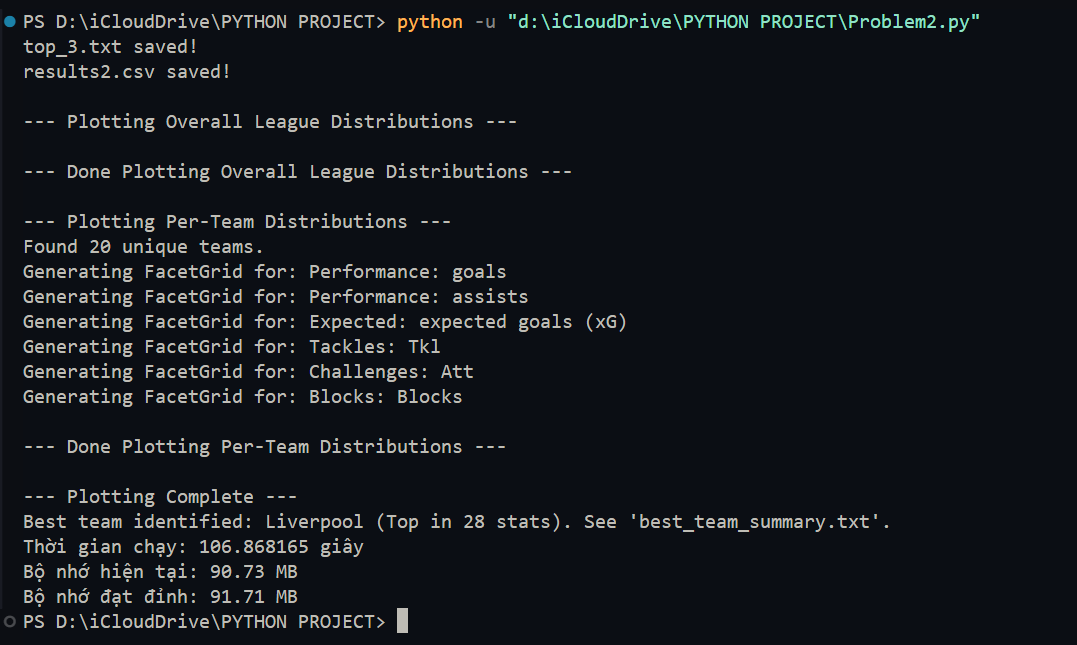
\includegraphics[width=300px]{Terminal_2.png}
    \caption{Terminal sau khi chạy chương trình Problem2.py}
    \label{fig:terminal2}
\end{figure}
Đoạn terminal cho thấy quá trình thực thi thành công của script Python \texttt{Problem2.py}. Trong quá trình chạy, chương trình đã lưu hai tệp kết quả là \texttt{top\_3.txt} và \texttt{results2.csv}, sau đó thực hiện vẽ biểu đồ phân phối dữ liệu cho toàn giải đấu và cho từng đội bóng. Có tổng cộng 20 đội được nhận diện, và biểu đồ được tạo cho nhiều chỉ số như \texttt{goals}, \texttt{assists}, \texttt{expected goals (xG)}, \texttt{tackles (Tkl)}, \texttt{challenges (Att)} và \texttt{blocks}. Kết quả phân tích cho thấy đội \texttt{Liverpool} là đội xuất sắc nhất, dẫn đầu ở 28 chỉ số. Thông tin chi tiết được lưu vào tệp \texttt{best\_team\_summary.txt}. Quá trình xử lý hoàn tất sau khoảng 106.87 giây với mức sử dụng bộ nhớ tối đa là 91.71 MB.\\

\begin{figure}[h]
    \centering
    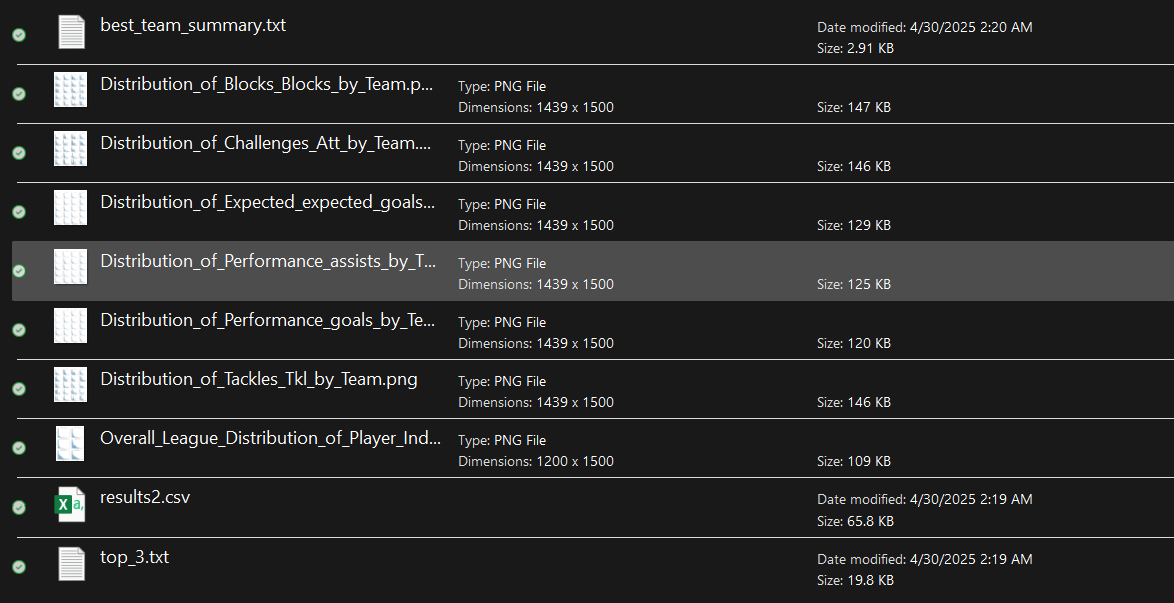
\includegraphics[width=300px]{P2_RES.png}
    \caption{Các tệp đầu ra sau khi chạy chương trình Problem2.py}
    \label{fig:output}
\end{figure}
Đầu ra chương trình gồm có 10 tệp, trong đó có 2 tệp đuôi txt, 1 tệp đuôi csv, 7 tệp đuôi png. Ở tệp top\_3.txt chứa dữ liệu đầu ra của function tìm top 3 người cao nhất và thấp nhất của mỗi chỉ số. Tệp results2.csv là đầu ra của function thống kê trung bình, trung vị và độ lệch của mỗi team theo yêu cầu đầu ra. Các file đuôi png là hình gồm 1 hình tổng hợp 6 thuộc tính cảu tất cả các cầu thủ chứa 6 biểu đồ, 6 hình còn lại mỗi hình chứa 20 biểu đồ là thống kê theo 6 thuộc tính của mỗi team. Đây cũng là kết quả đầu ra chủa chương trình vẽ đồ thị. File txt cuối cùng là kết quả đầu ra của chương trình tìm ra team cao nhất ở mỗi thuộc tính và dự đoán team có thành tích tốt nhất của mùa giải.
\subsubsection{Chi tiết kết quả đầu ra}
\textbf{top\_3.txt}
Tệp này cung cấp một phân tích định lượng chi tiết về hiệu suất của cầu thủ trong một giải đấu bóng đá, được sắp xếp theo các danh mục thống kê. Mỗi danh mục so sánh "Top 3 Highest" và "Top 3 Lowest" để làm nổi bật phạm vi hiệu suất. Các danh mục bao gồm thời gian thi đấu, hiệu suất (ví dụ: bàn thắng, kiến tạo), chỉ số kỳ vọng (ví dụ: xG, xAG), chỉ số tiến triển, số liệu thống kê trên 90 phút, số liệu thống kê tiêu chuẩn, số liệu thống kê về chuyền bóng, các đường chuyền quan trọng, các hành động tạo ra cú sút, tắc bóng và tranh chấp, đánh chặn và phá bóng, chạm bóng, rê bóng, chuyền bóng, nhận bóng và phạm lỗi. Nhìn chung, tệp cung cấp một cái nhìn có cấu trúc về điểm mạnh và điểm yếu của cầu thủ.\\
\begin{figure}[h]
    \centering
    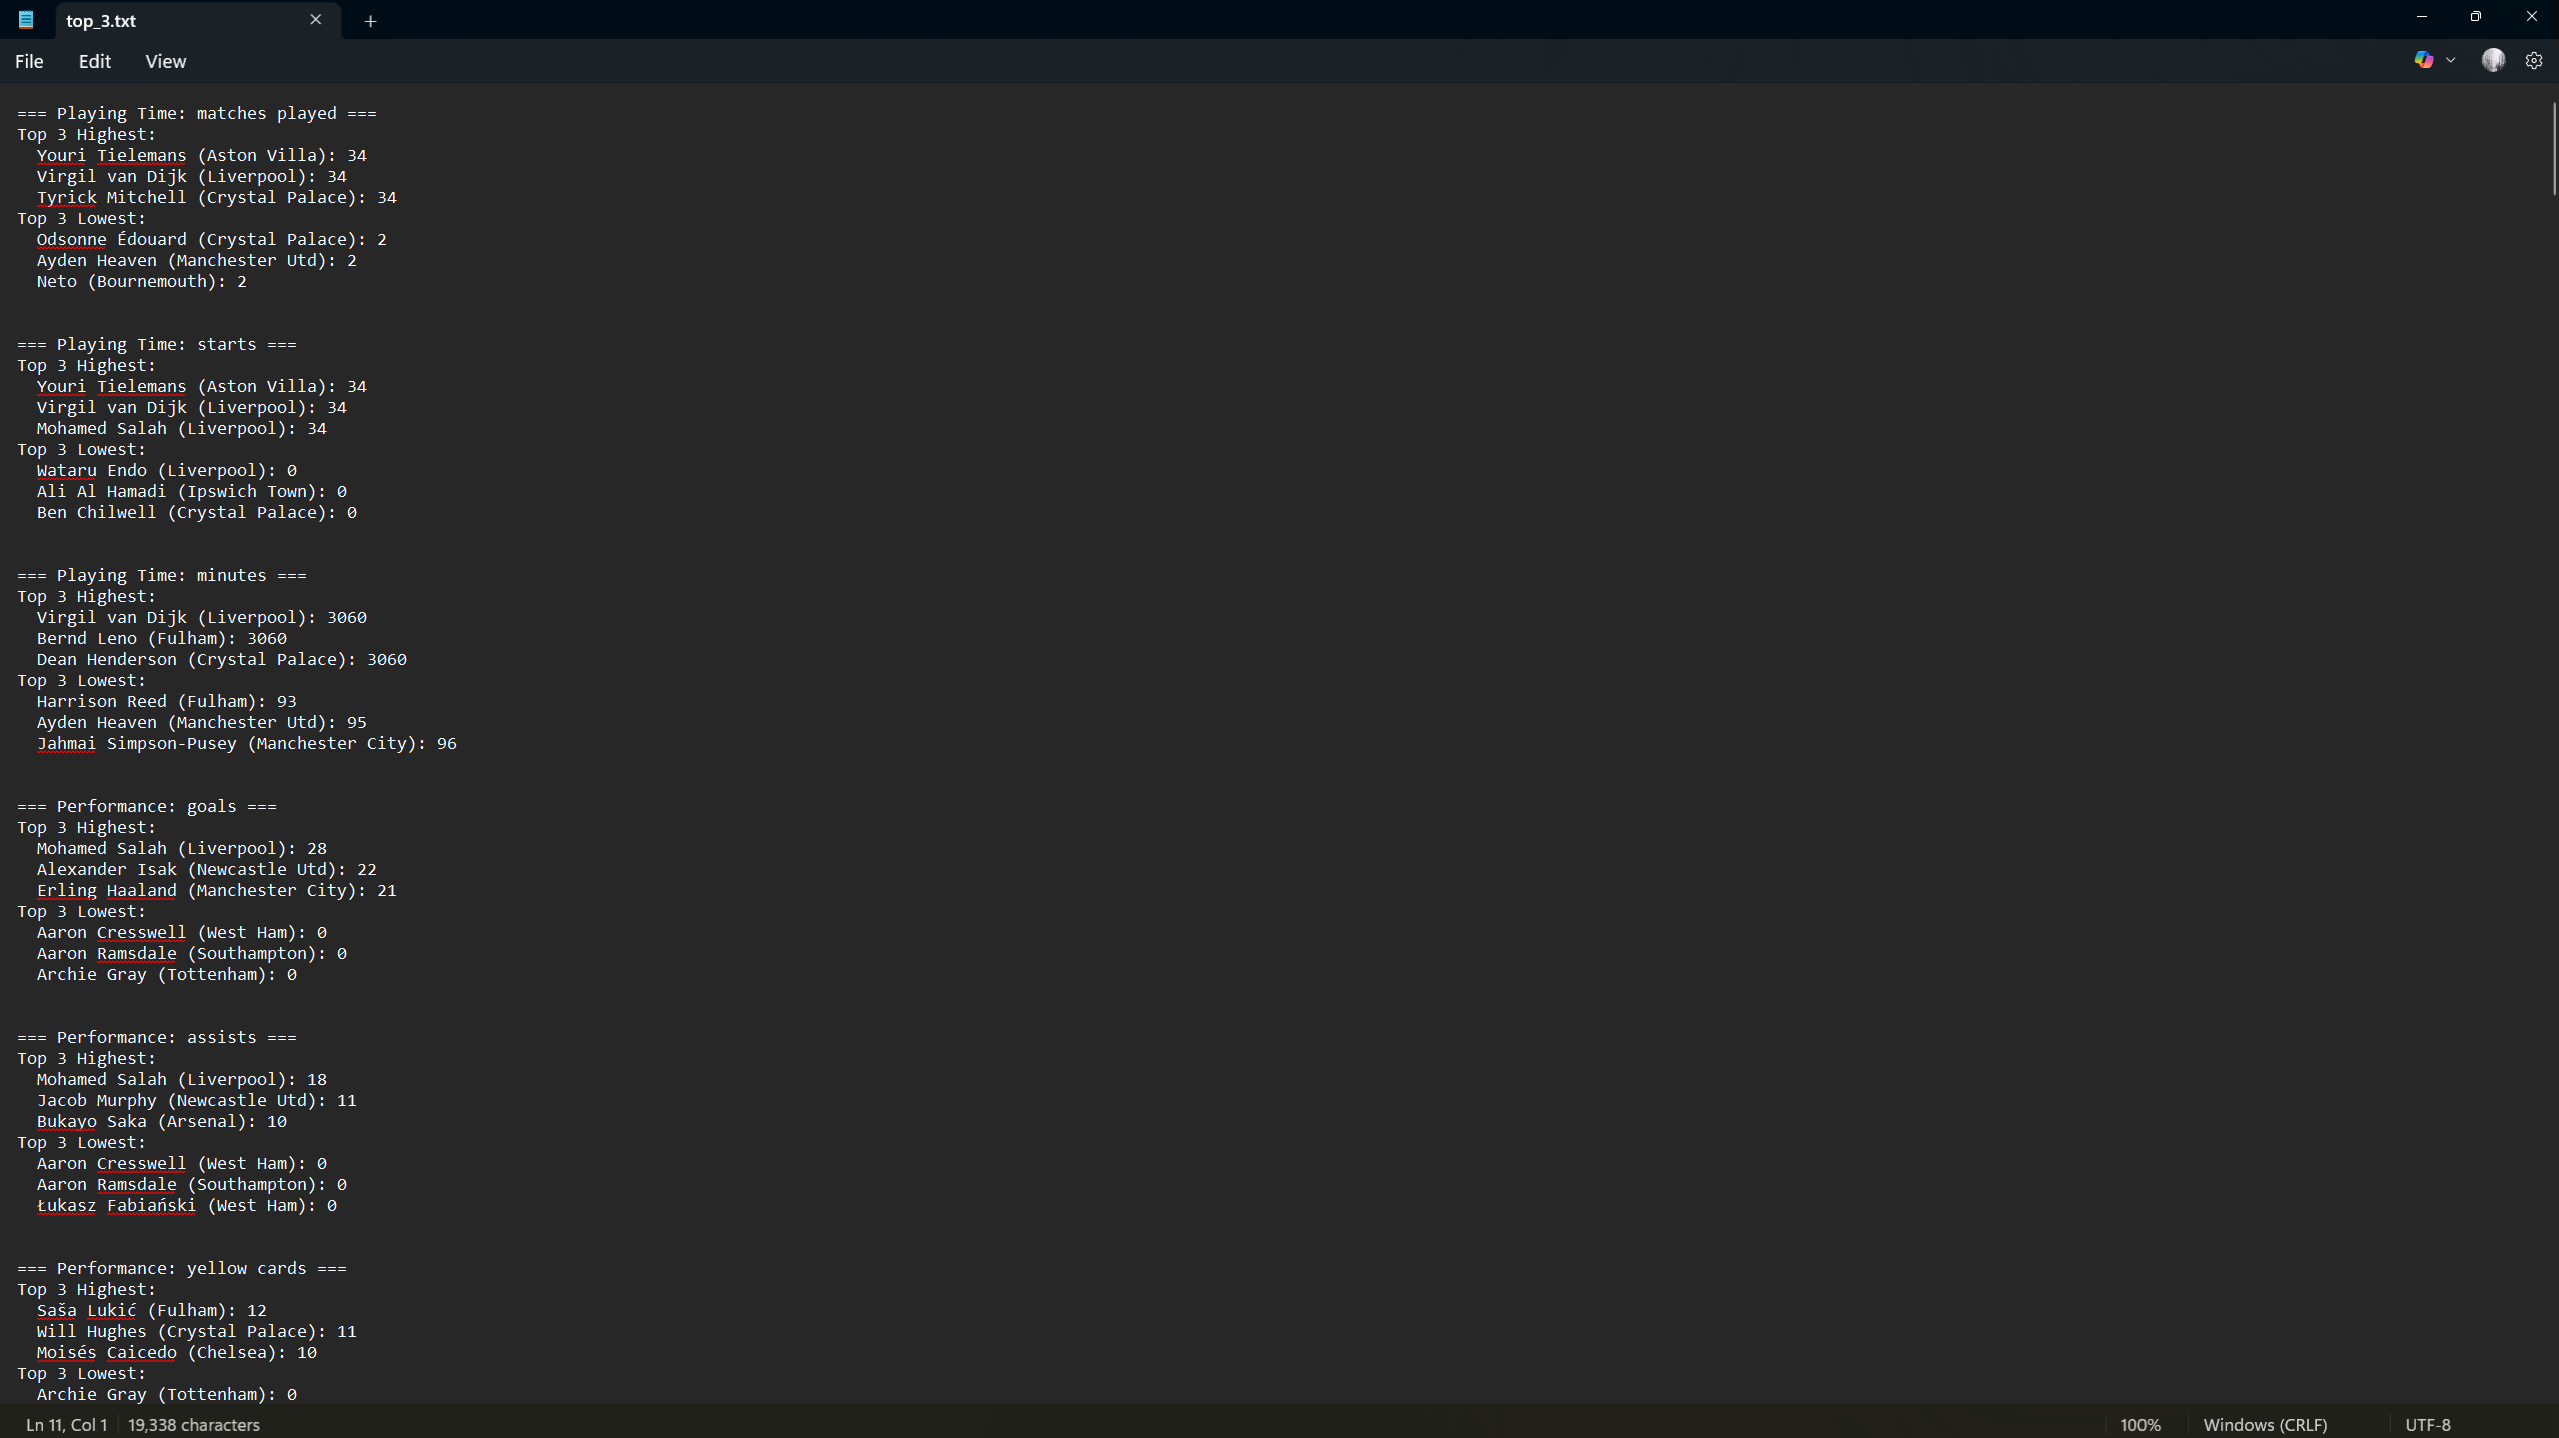
\includegraphics[width=220px]{top_3.png}
    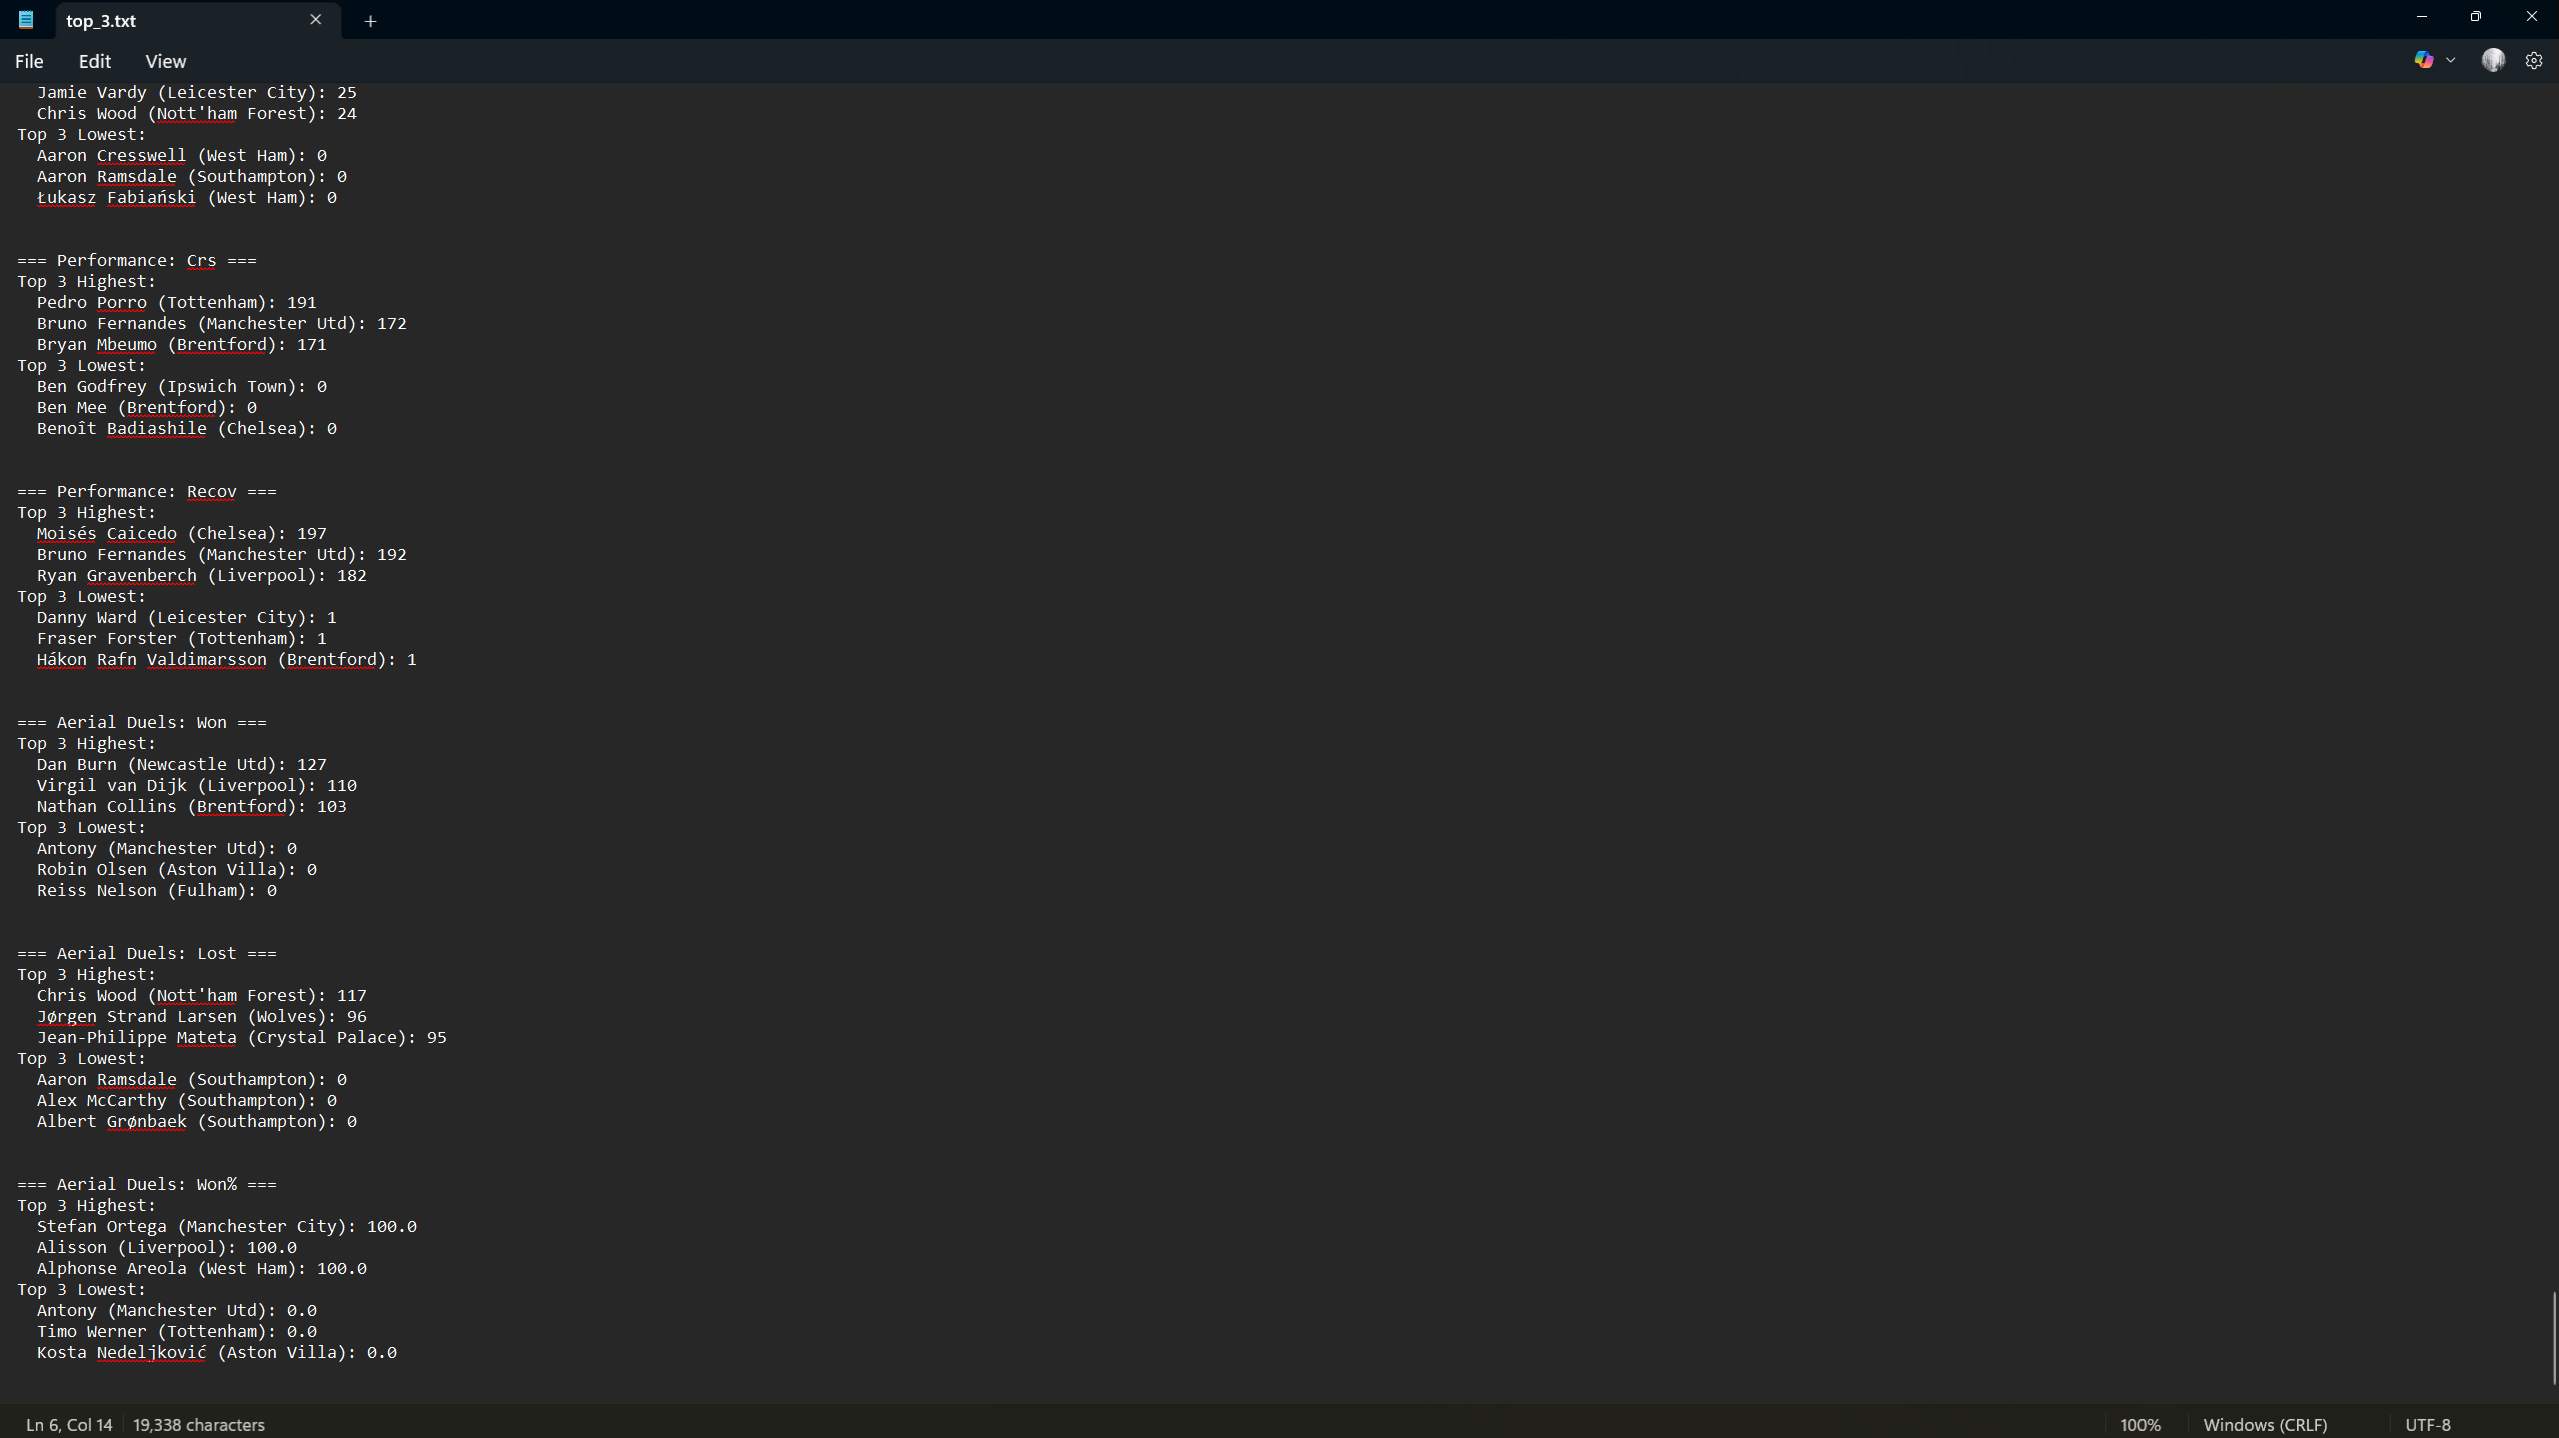
\includegraphics[width=220px]{top_3_1.png}
    \caption{File top\_3.txt}
    \label{fig:top3}
\end{figure}
\textbf{results2.csv}
Tệp results2.csv chứa dữ liệu thống kê tổng hợp về các đội bóng trong một giải đấu, với tổng cộng 21 đội (hoặc nhóm) và 220 cột đặc trưng liên quan đến hiệu suất thi đấu. Mỗi hàng đại diện cho một đội, bao gồm tên đội và các chỉ số mô tả trung vị, trung bình, độ lệch chuẩn của nhiều khía cạnh trong thi đấu.\\
Các thông số được ghi nhận bao gồm:
\begin{itemize}
	\item Thời gian thi đấu: số trận ra sân, số trận đá chính, tổng phút thi đấu;
	\item Chỉ số thi đấu kỹ thuật: như số pha không chiến thắng/thua, tỷ lệ thắng không chiến;
	\item Dạng thống kê: mỗi chỉ số thường có 3 biến đi kèm – giá trị trung vị (Median), trung bình (Mean) và độ lệch chuẩn (Std), thể hiện sự phân tán trong tập dữ liệu.
\end{itemize}
\begin{figure}[h]
    \centering
    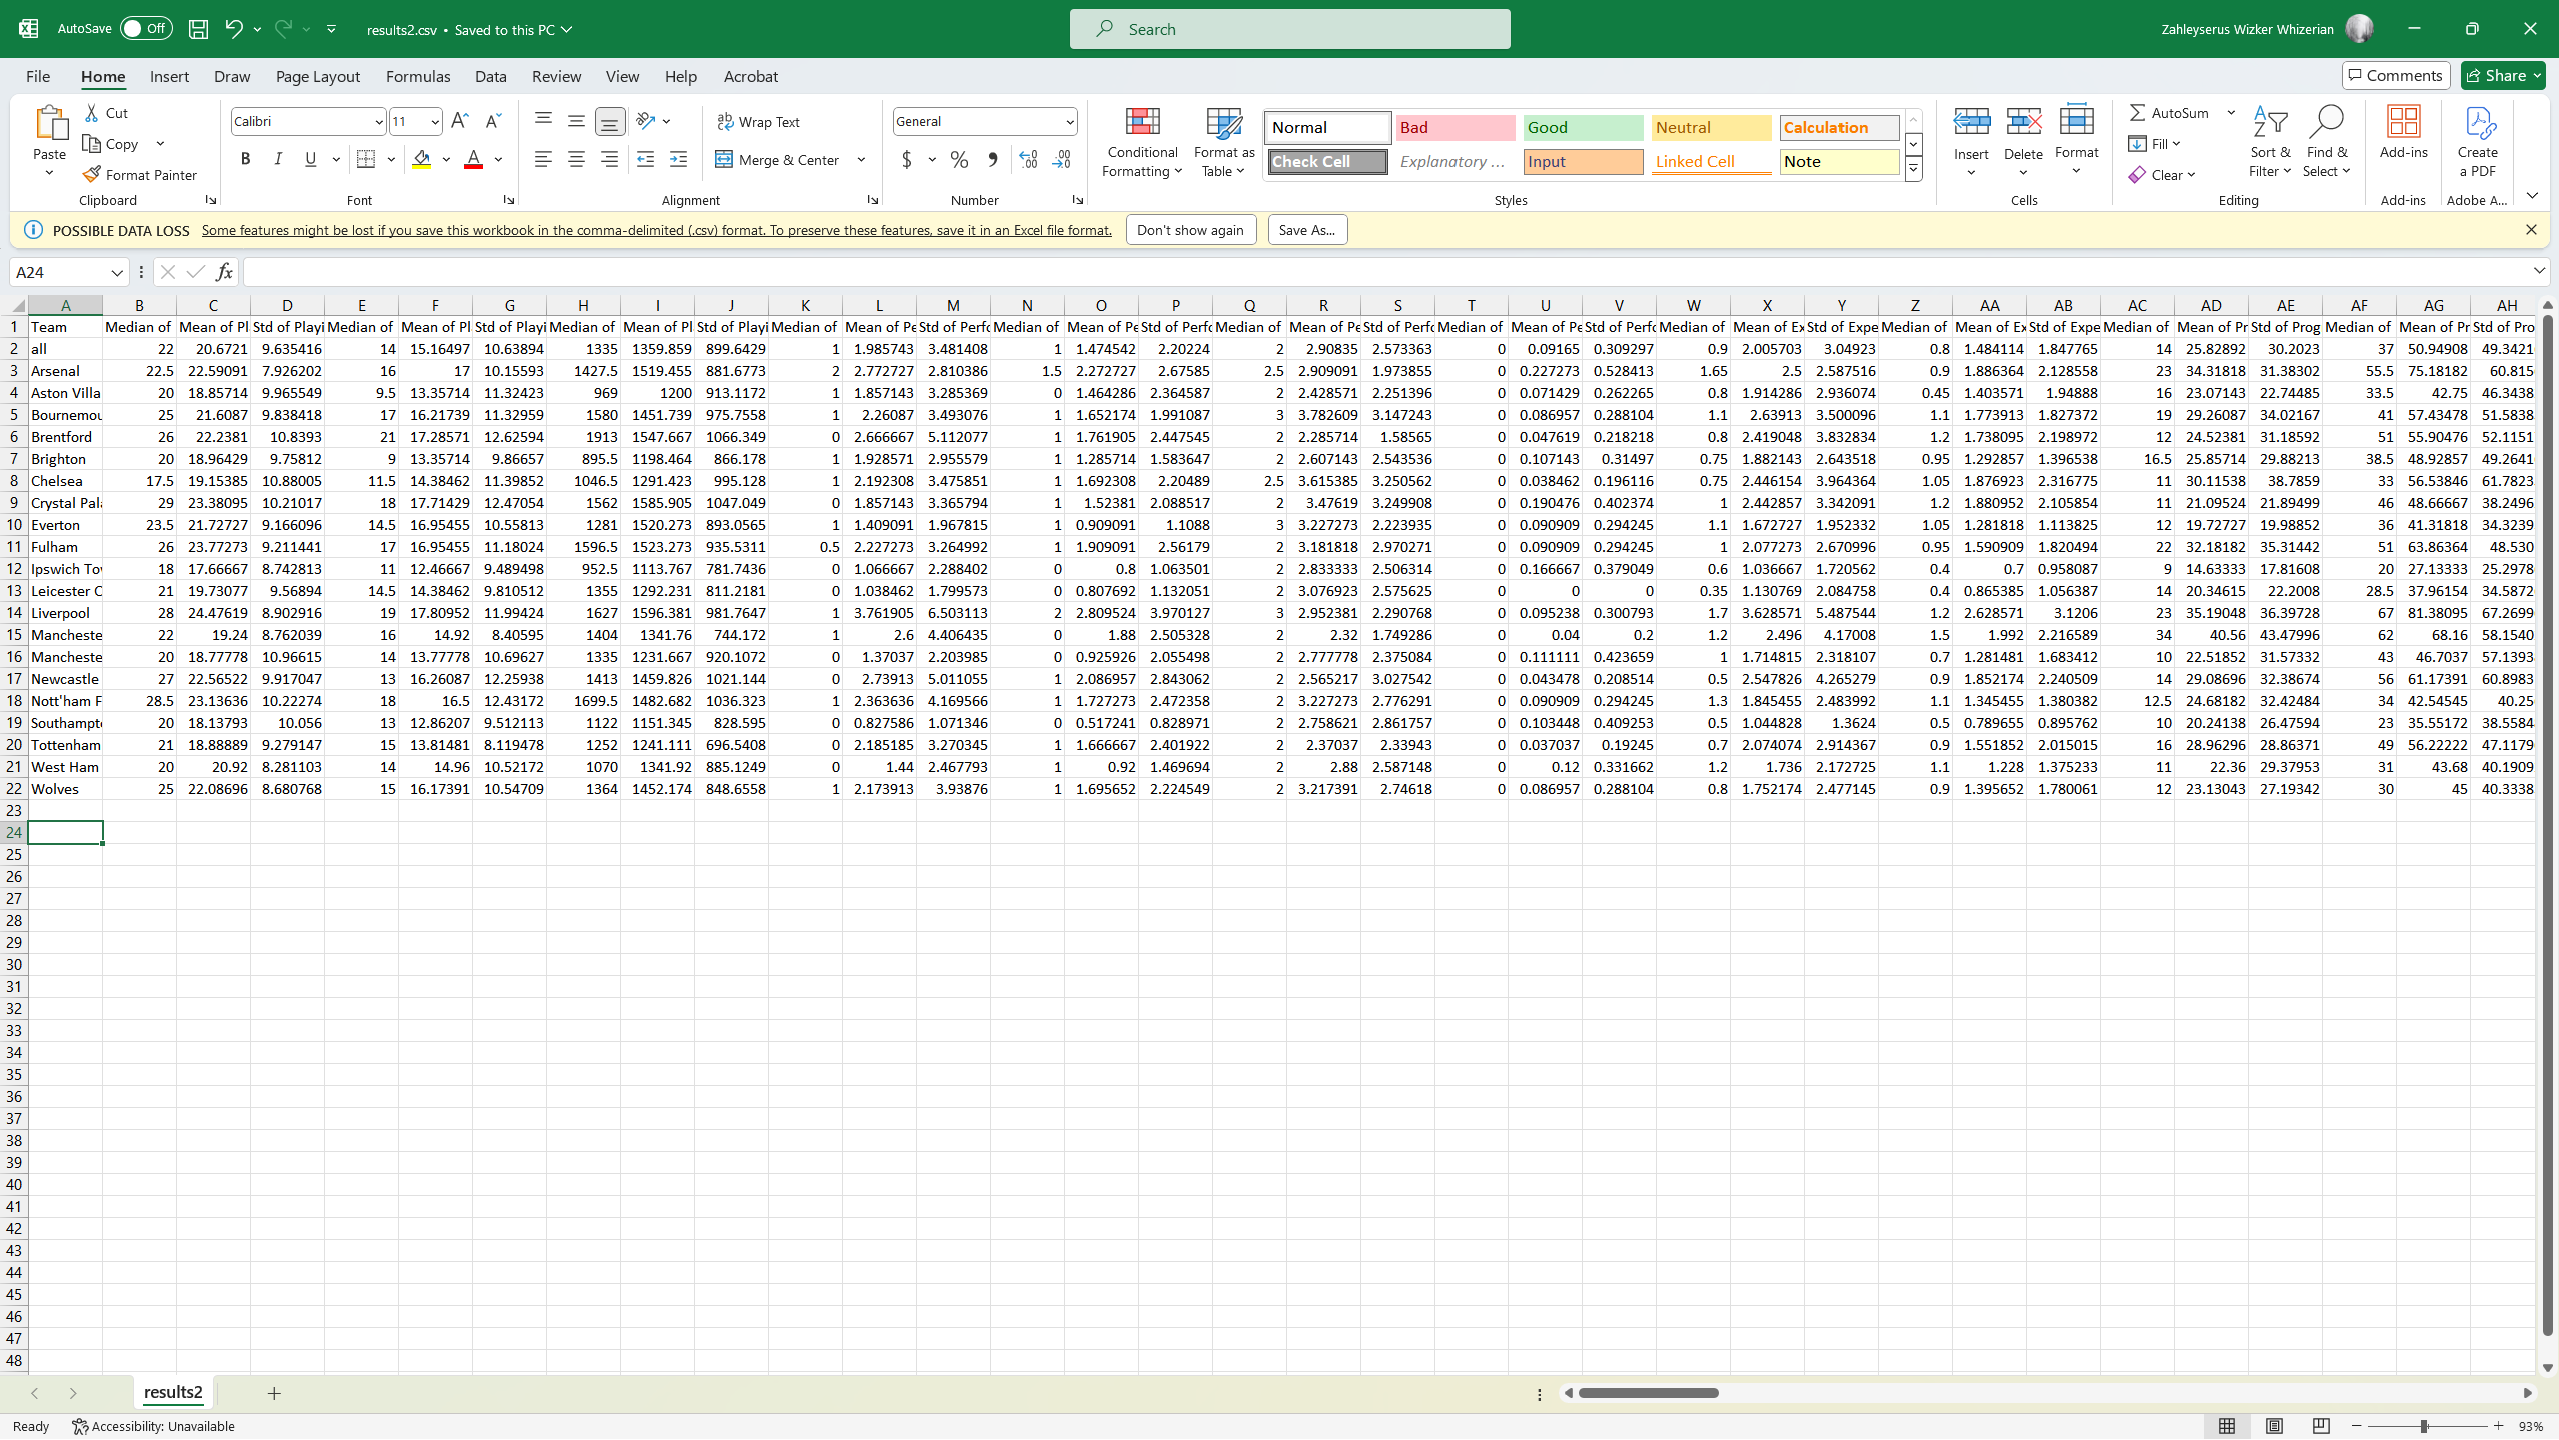
\includegraphics[width=220px]{results2.png}
    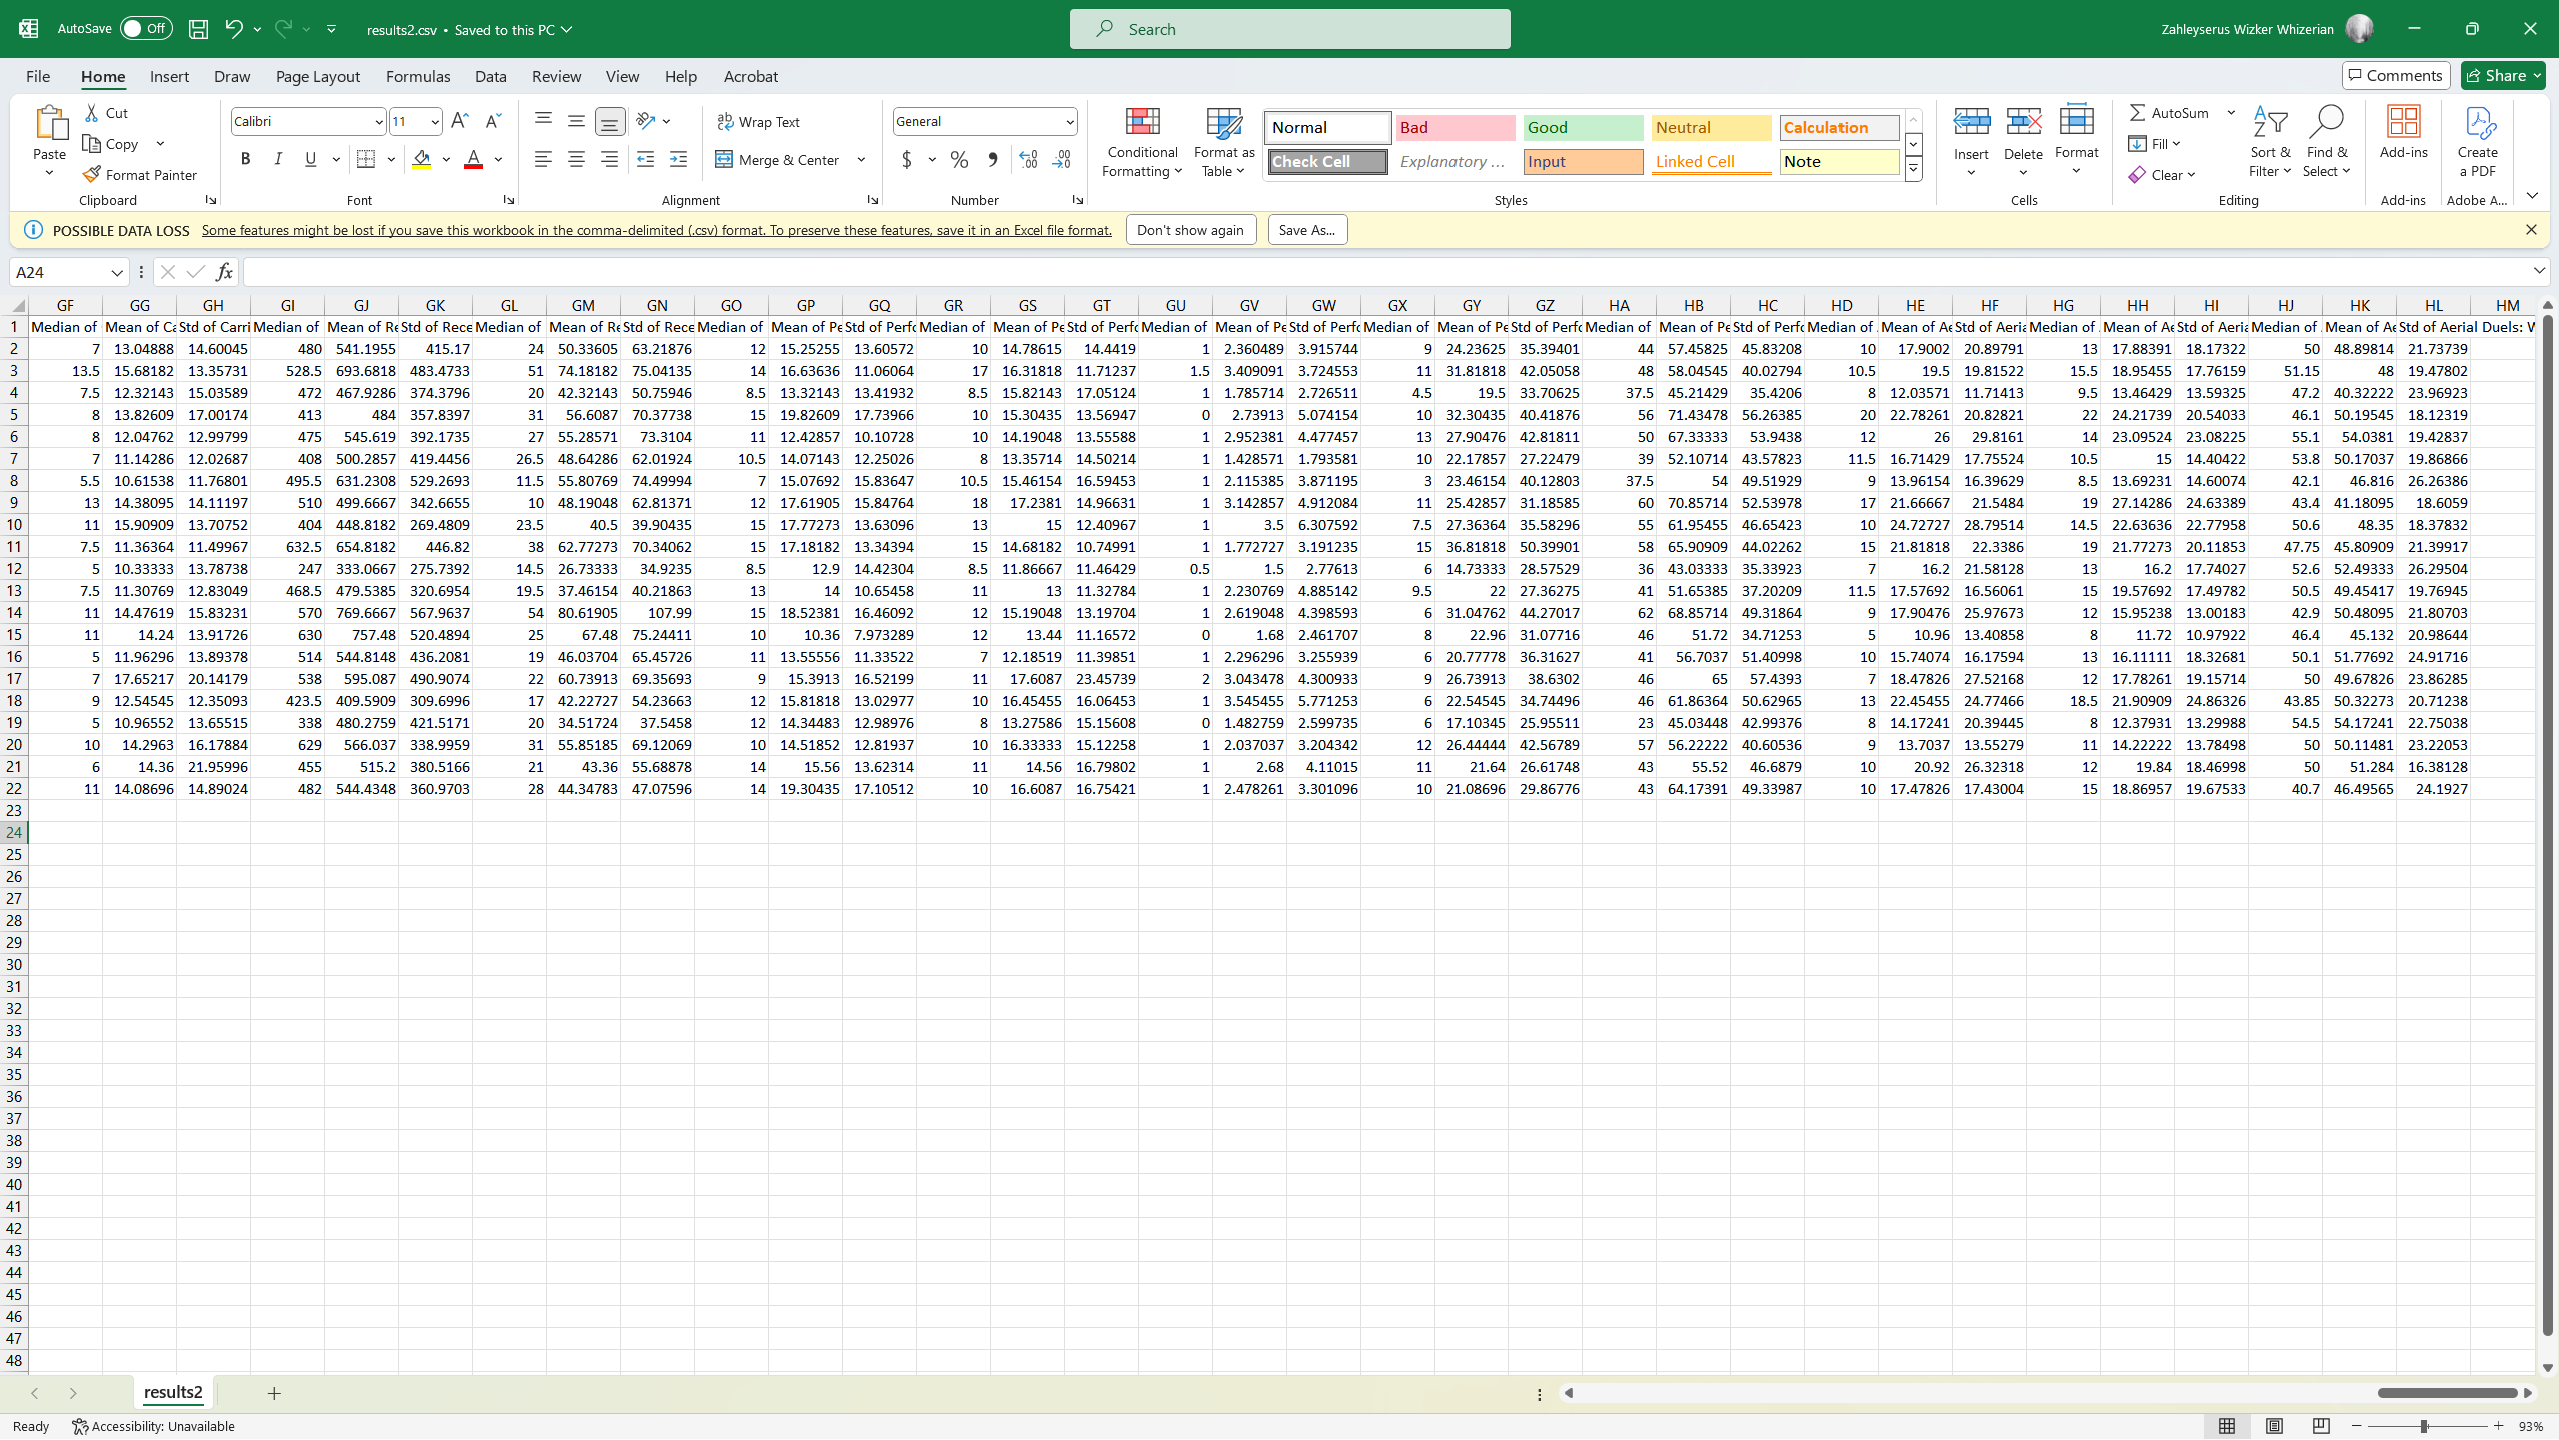
\includegraphics[width=220px]{results2_1.png}
    \caption{File results2.csv}
    \label{fig:res2}
\end{figure}
\textbf{Overall\_League\_Distribution\_of\_Player\_Indexes.png}
Hình ảnh gồm 6 biểu đồ histogram được bố trí theo dạng lưới 2 cột × 3 hàng, mỗi biểu đồ có:
\begin{itemize}
	\item Tiêu đề rõ ràng ở phía trên, mô tả tên chỉ số được thể hiện (ví dụ: Distribution of Performance: goals).
	\item Trục hoành (X-axis) hiển thị tên chỉ số cụ thể (như Performance: goals, Tackles: Tkl).
	\item Trục tung (Y-axis) được gán nhãn là Frequency, biểu thị tần suất xuất hiện.
	\item Các cột histogram màu xanh nhạt minh họa phân bố dữ liệu.
\end{itemize}
Một đường cong KDE màu xanh đậm được vẽ mượt theo phân bố dữ liệu để trực quan hóa mật độ xác suất.
Toàn bộ hình ảnh có bố cục gọn gàng, đồng nhất về kiểu trình bày và định dạng trục, giúp dễ dàng so sánh giữa các biểu đồ.
\begin{figure}[h]
    \centering
    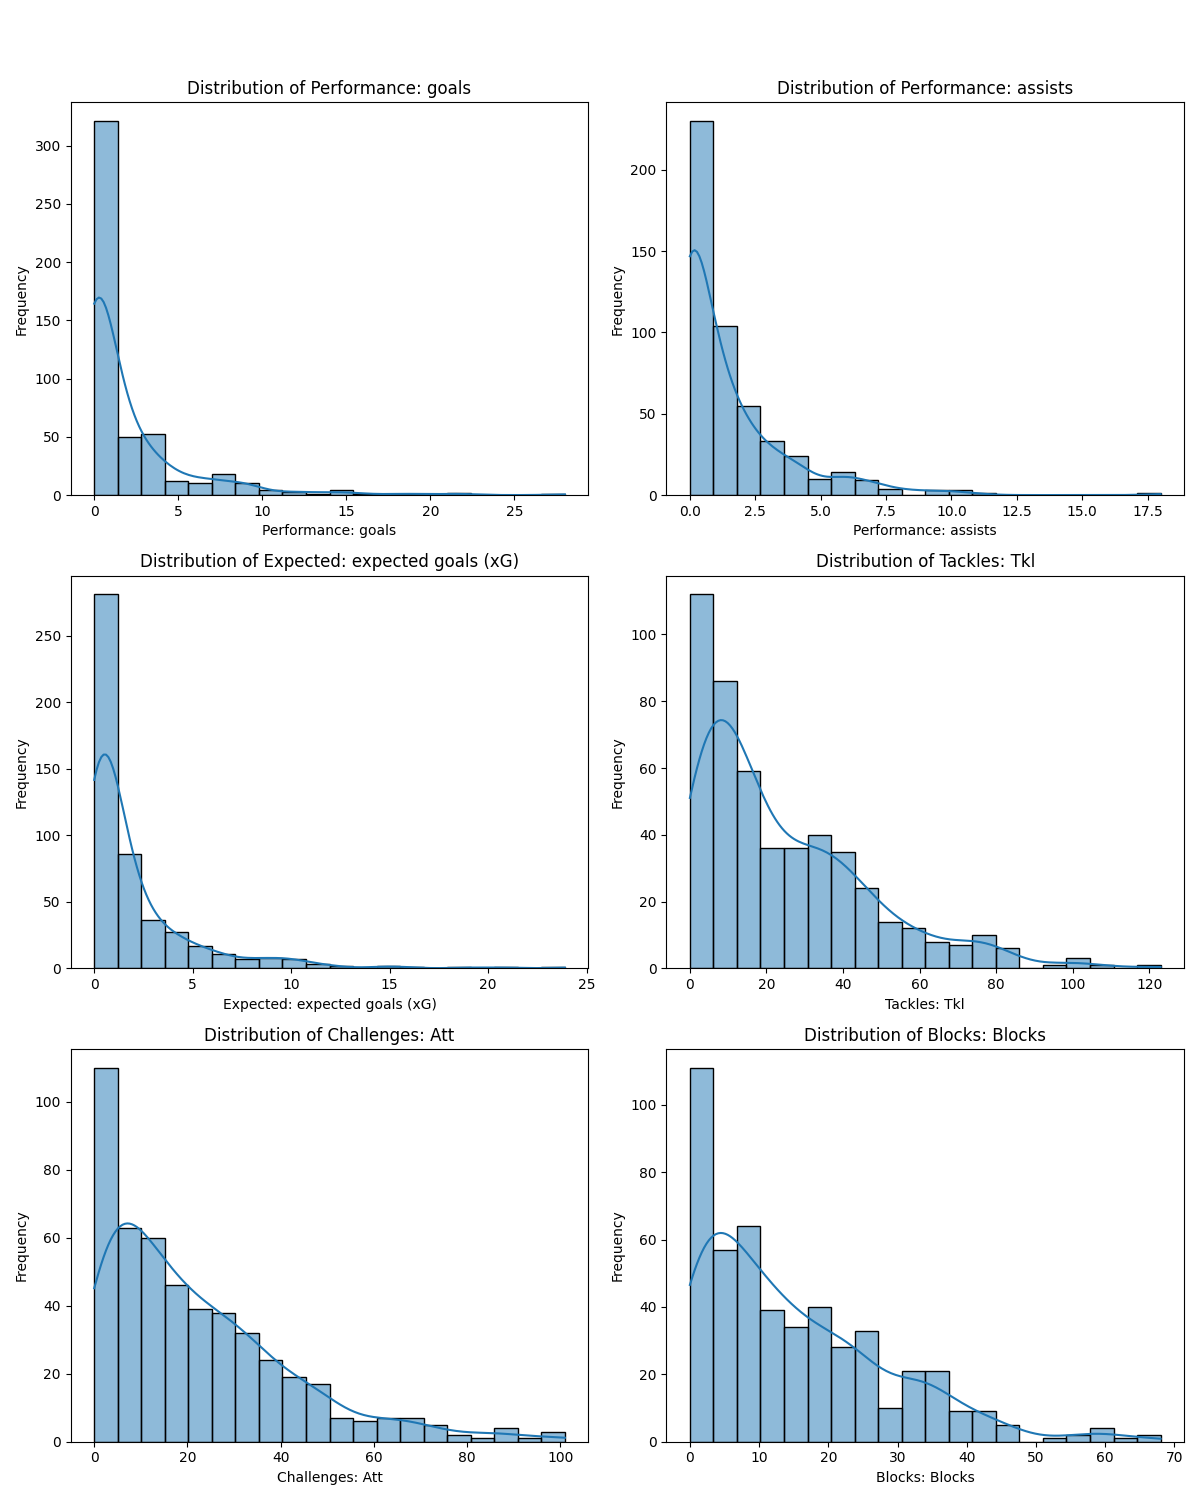
\includegraphics[width=400px]{Overall_League_Distribution_of_Player_Indexes.png}
    \caption{File Overall\_League\_Distribution\_of\_Player\_Indexes.png}
    \label{fig:p1}
\end{figure}
\begin{figure}[h]
    \centering
    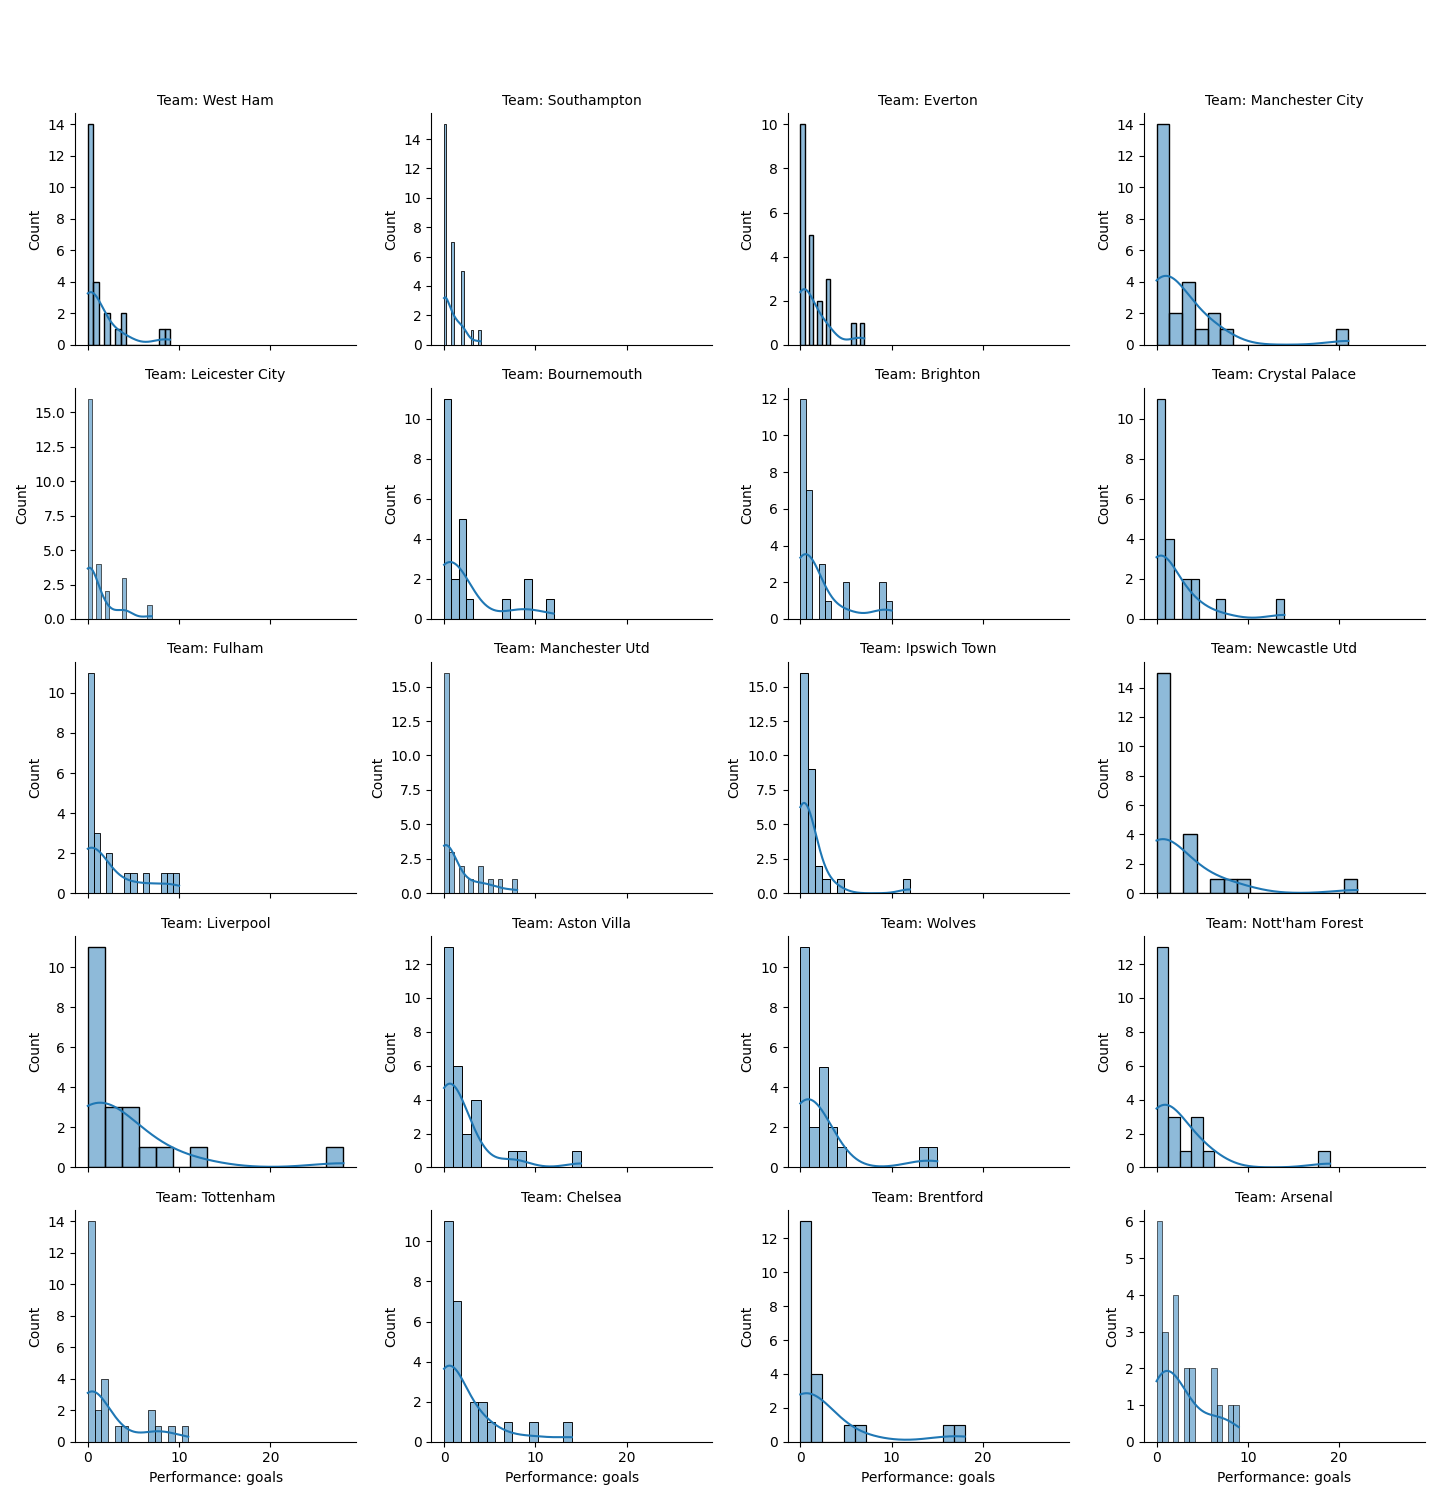
\includegraphics[width=300px]{Distribution_of_Performance_goals_by_Team.png}
    \caption{File Distribution\_of\_Performance\_goals\_by\_Team.png}
    \label{fig:p2}
\end{figure}
\begin{figure}[h]
    \centering
    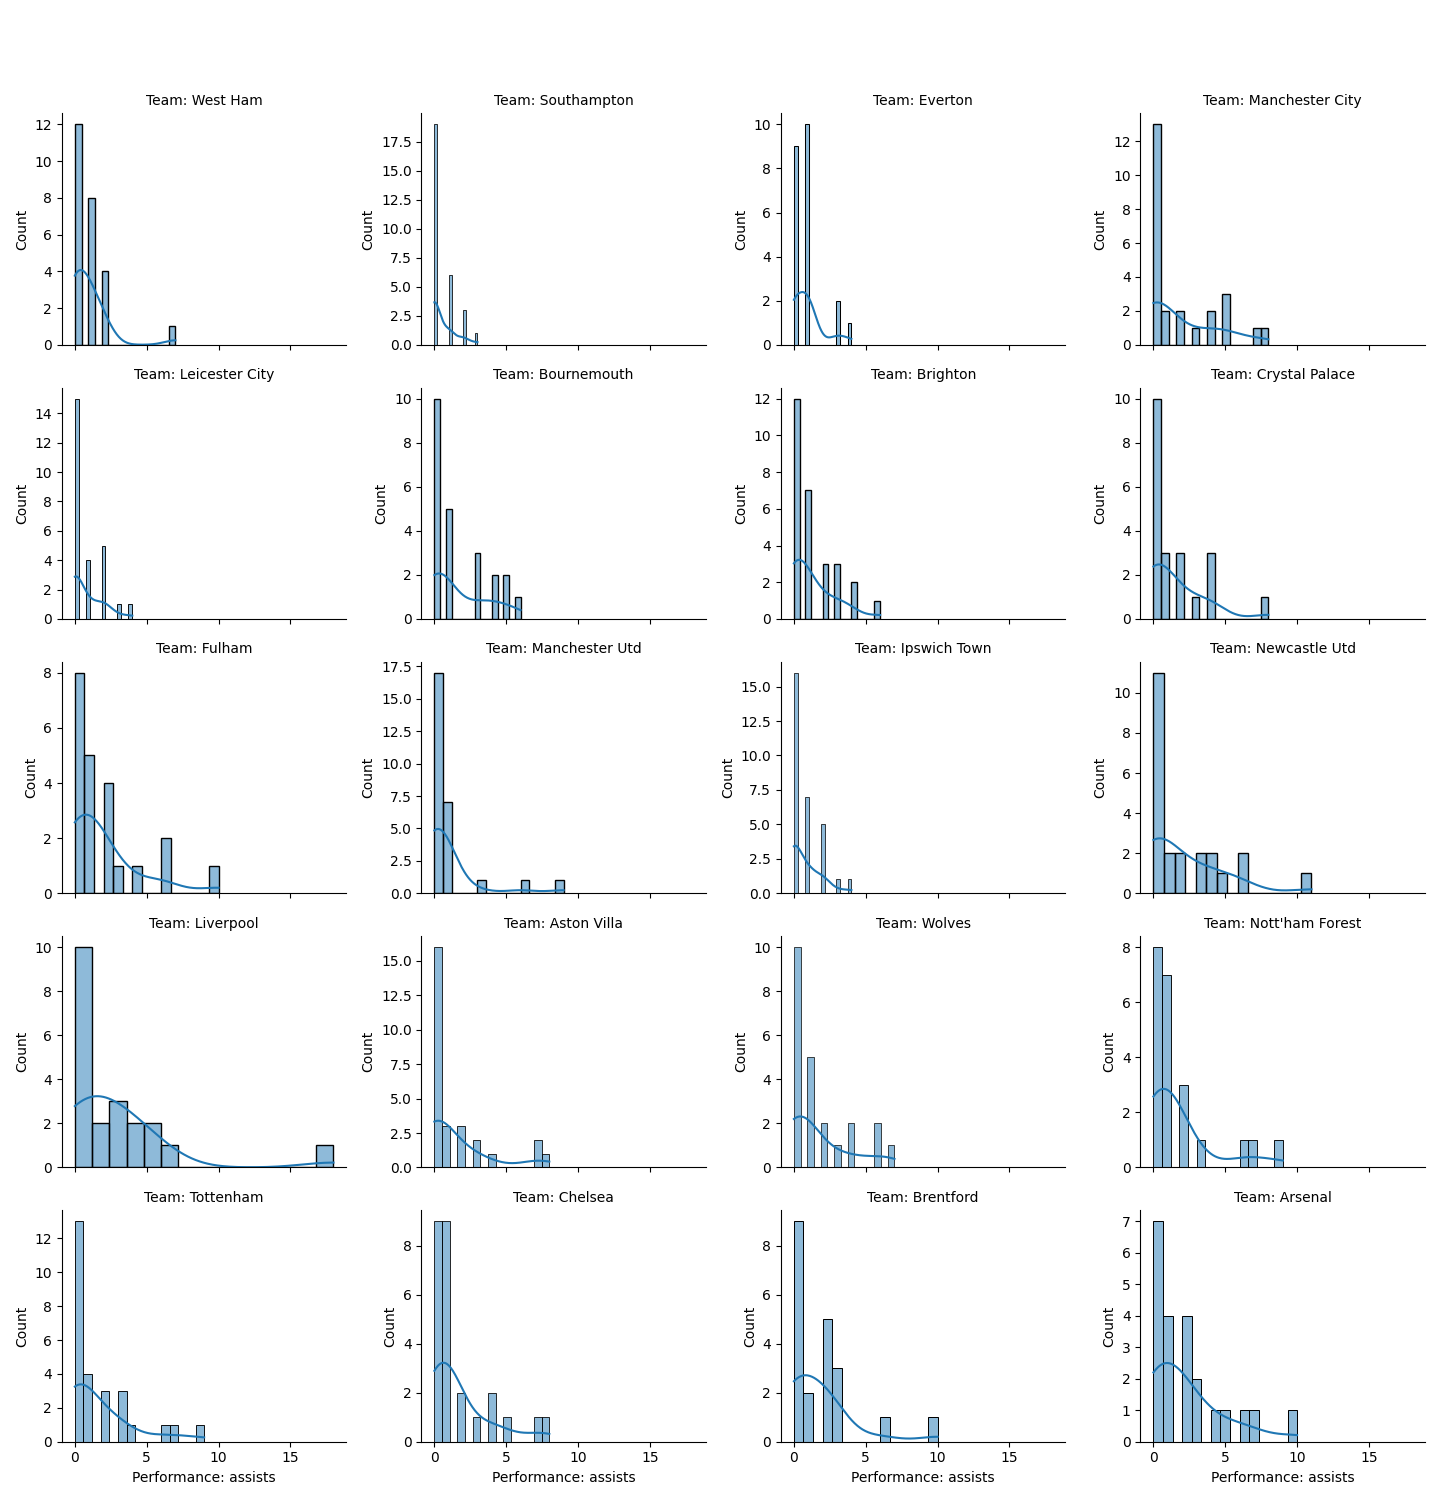
\includegraphics[width=300px]{Distribution_of_Performance_assists_by_Team.png}
    \caption{File Distribution\_of\_Performance\_assists\_by\_Team.png}
    \label{fig:p3}
\end{figure}
\begin{figure}[h]
    \centering
    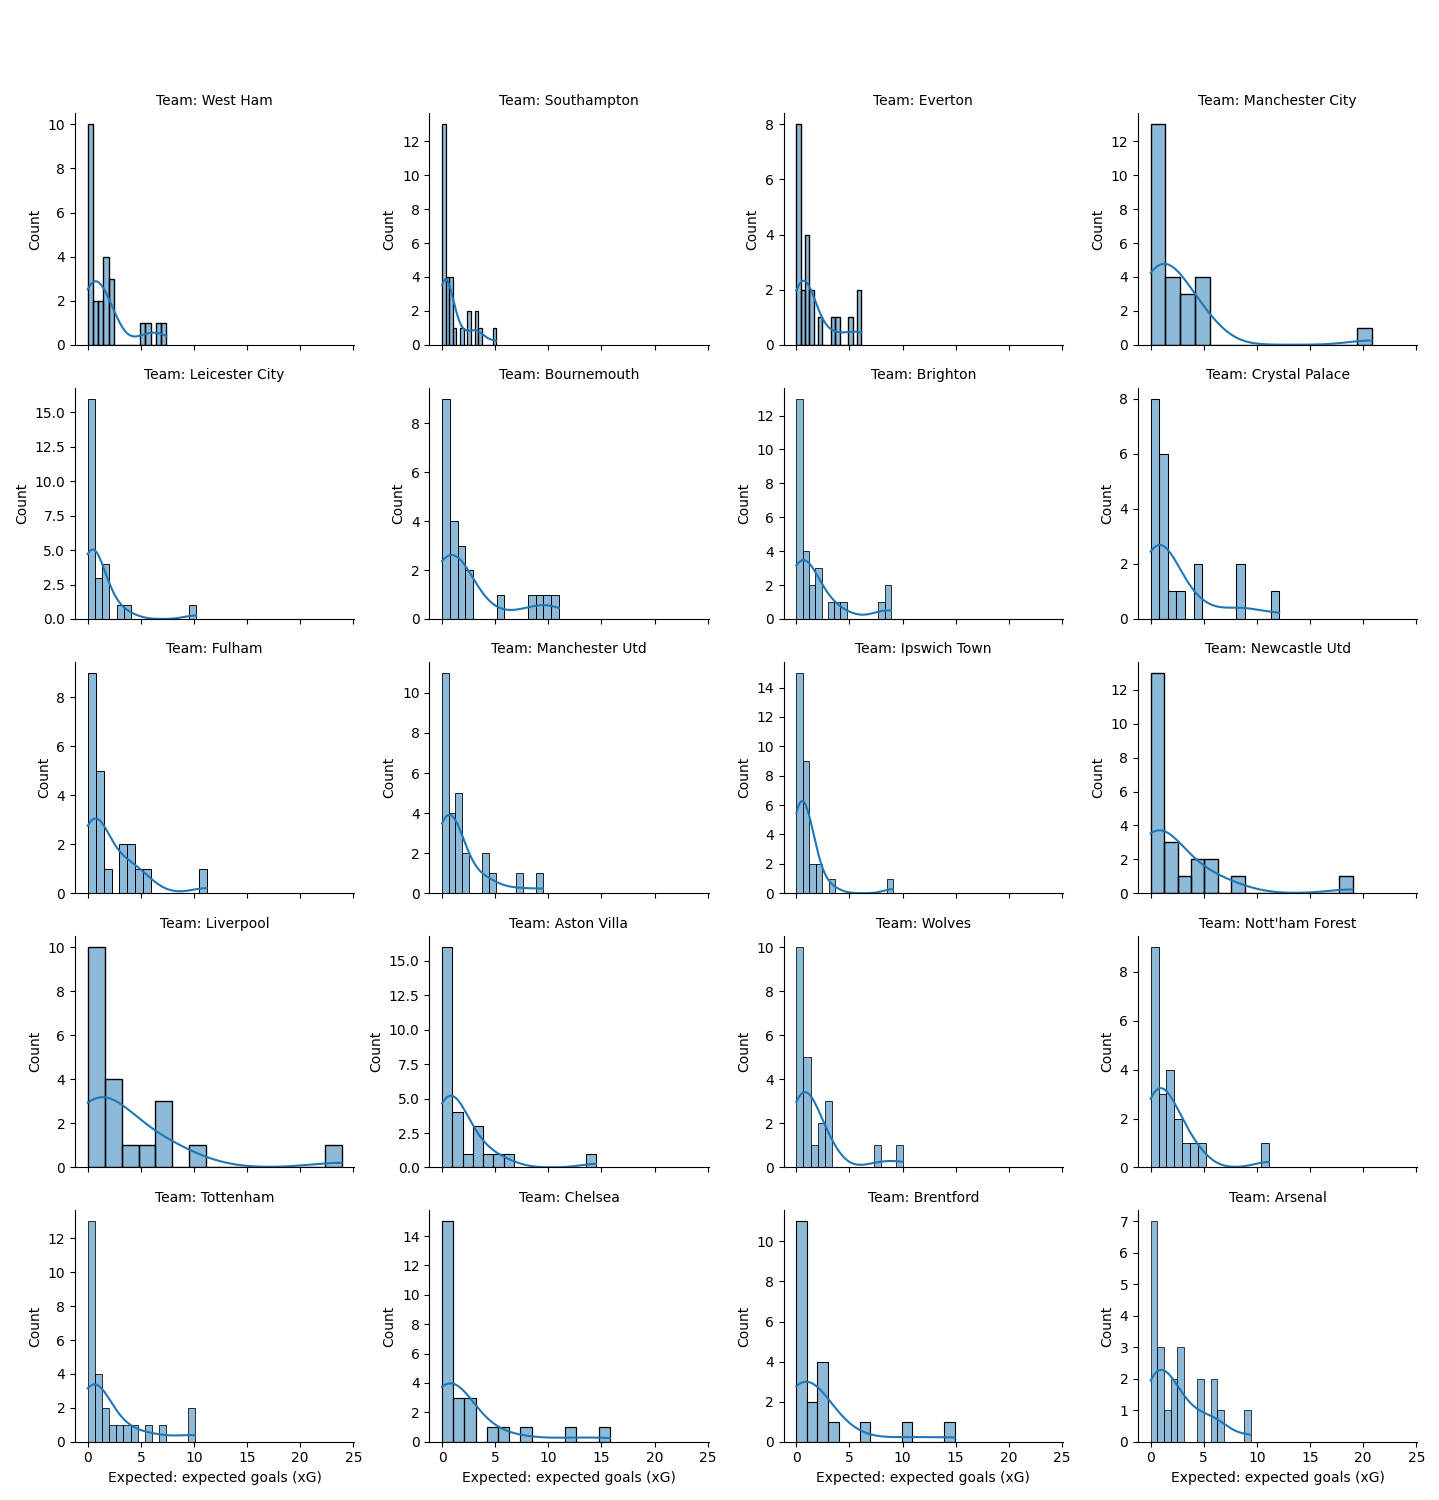
\includegraphics[width=300px]{Distribution_of_Expected_expected_goals_(xG)_by_Team.png}
    \caption{File Distribution\_of\_Expected\_expected\_goals\_(xG)\_by\_Team.png}
    \label{fig:p4}
\end{figure}
\begin{figure}[h]
    \centering
    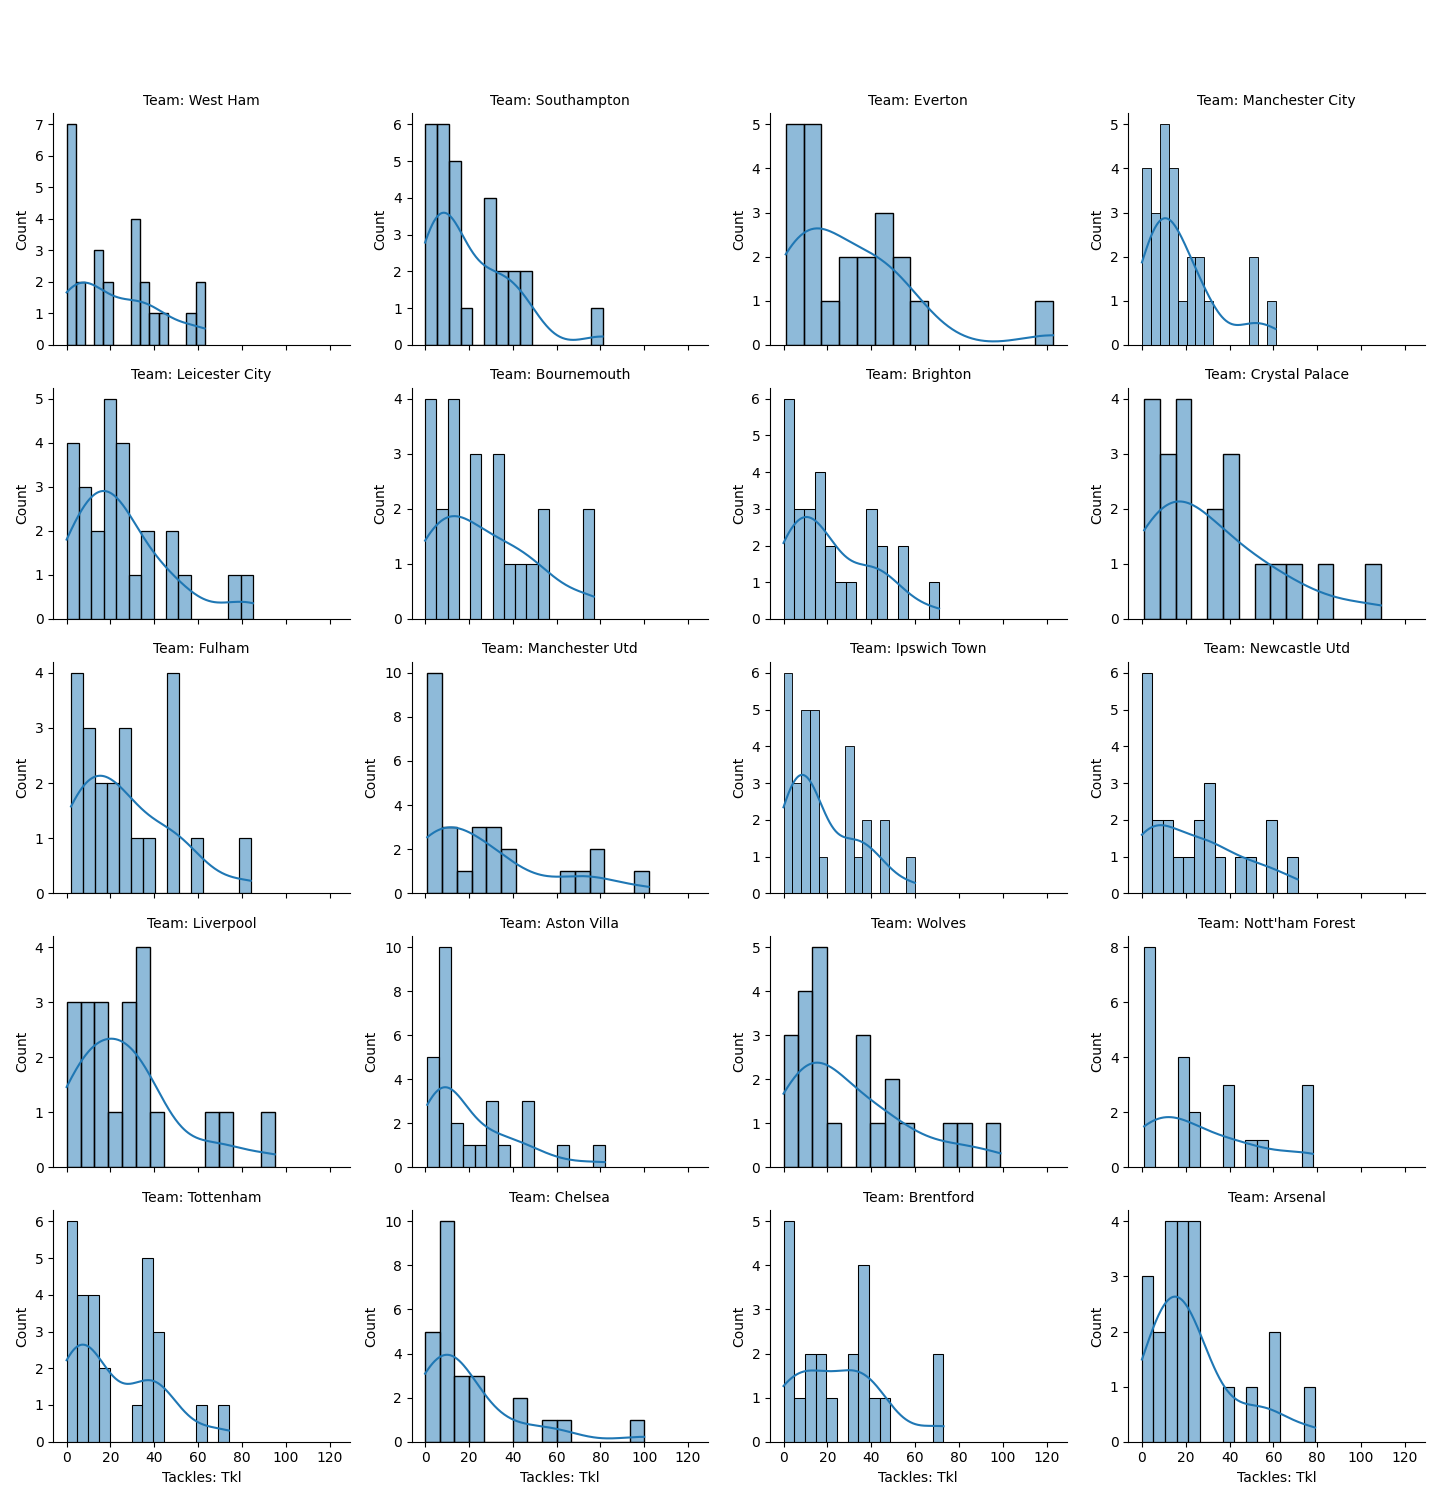
\includegraphics[width=300px]{Distribution_of_Tackles_Tkl_by_Team.png}
    \caption{File Distribution\_of\_Tackles\_Tkl\_by\_Team.png}
    \label{fig:p5}
\end{figure}
\begin{figure}[h]
    \centering
    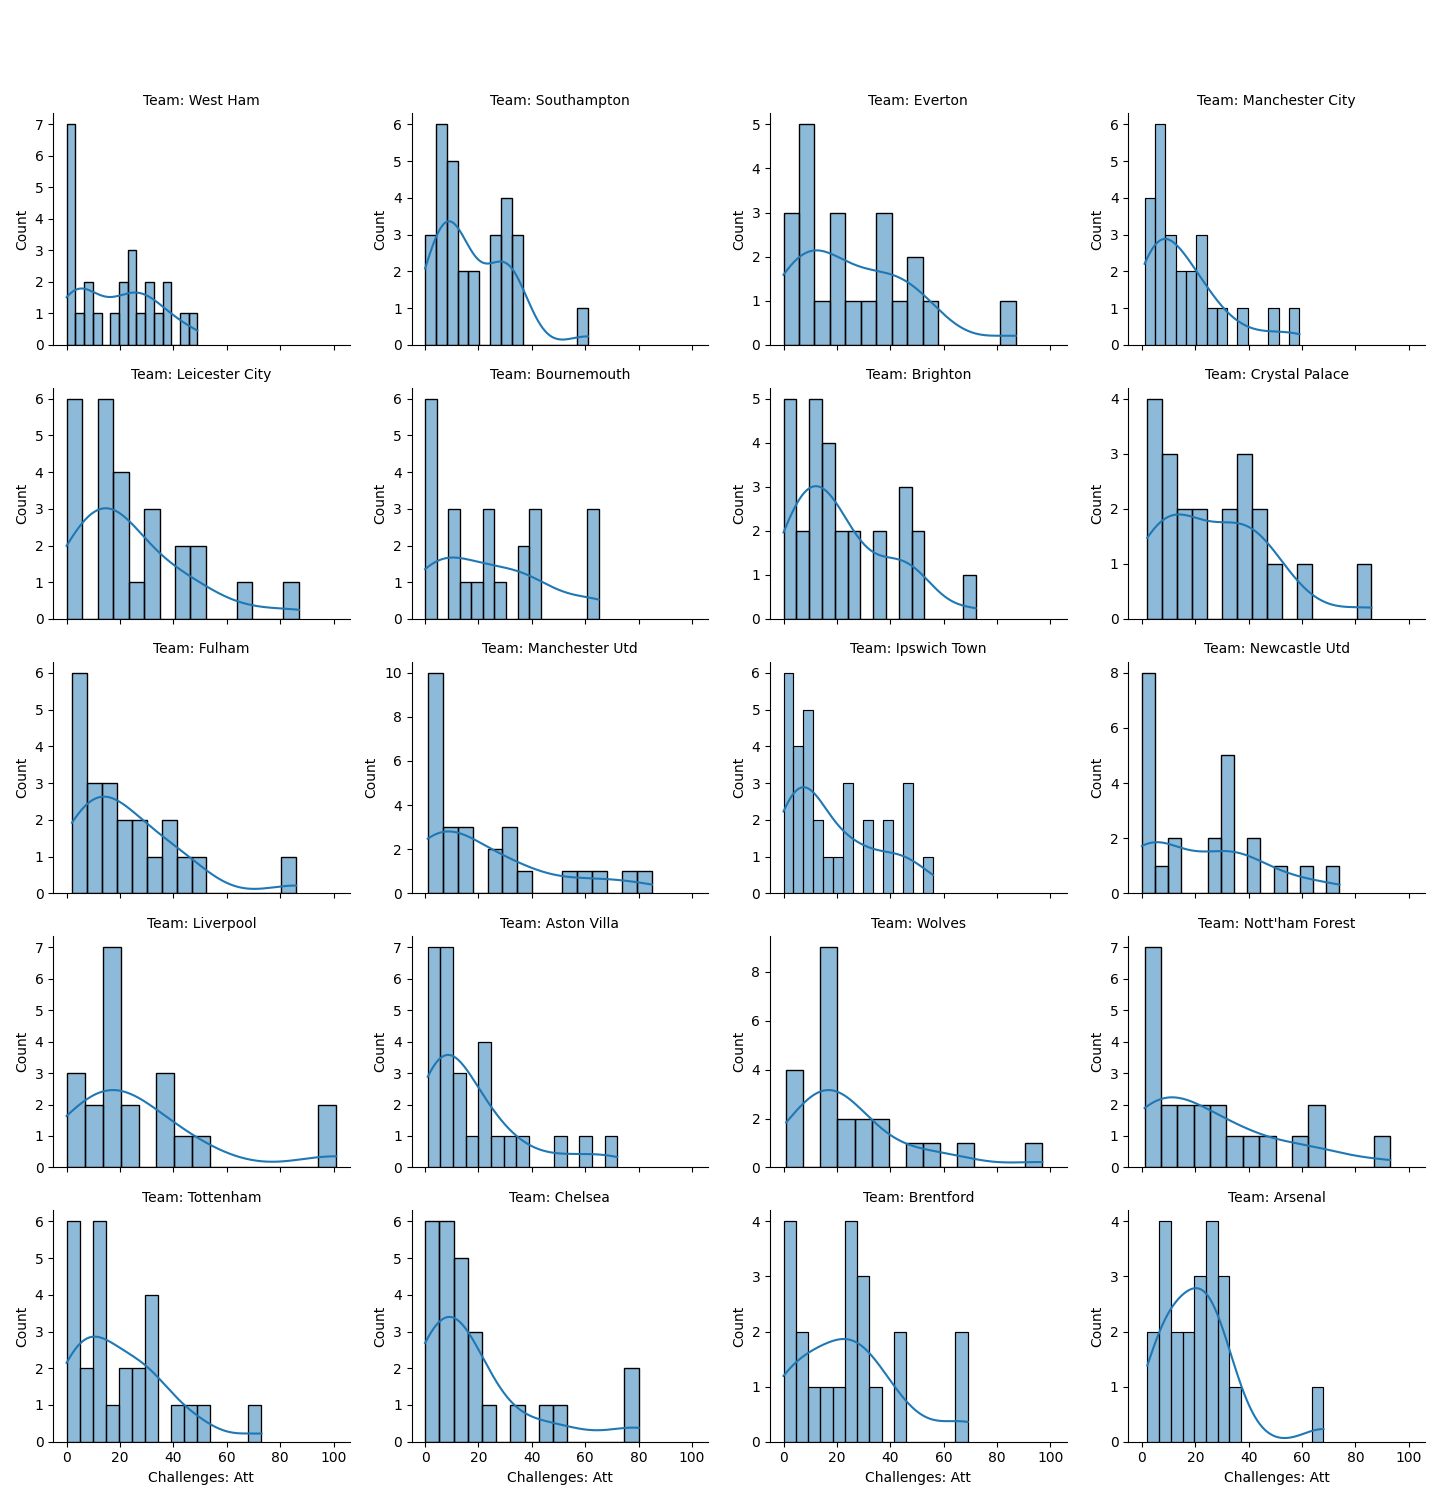
\includegraphics[width=300px]{Distribution_of_Challenges_Att_by_Team.png}
    \caption{File Distribution\_of\_Challenges\_Att\_by\_Team.png}
    \label{fig:p6}
\end{figure}
\begin{figure}[h]
    \centering
    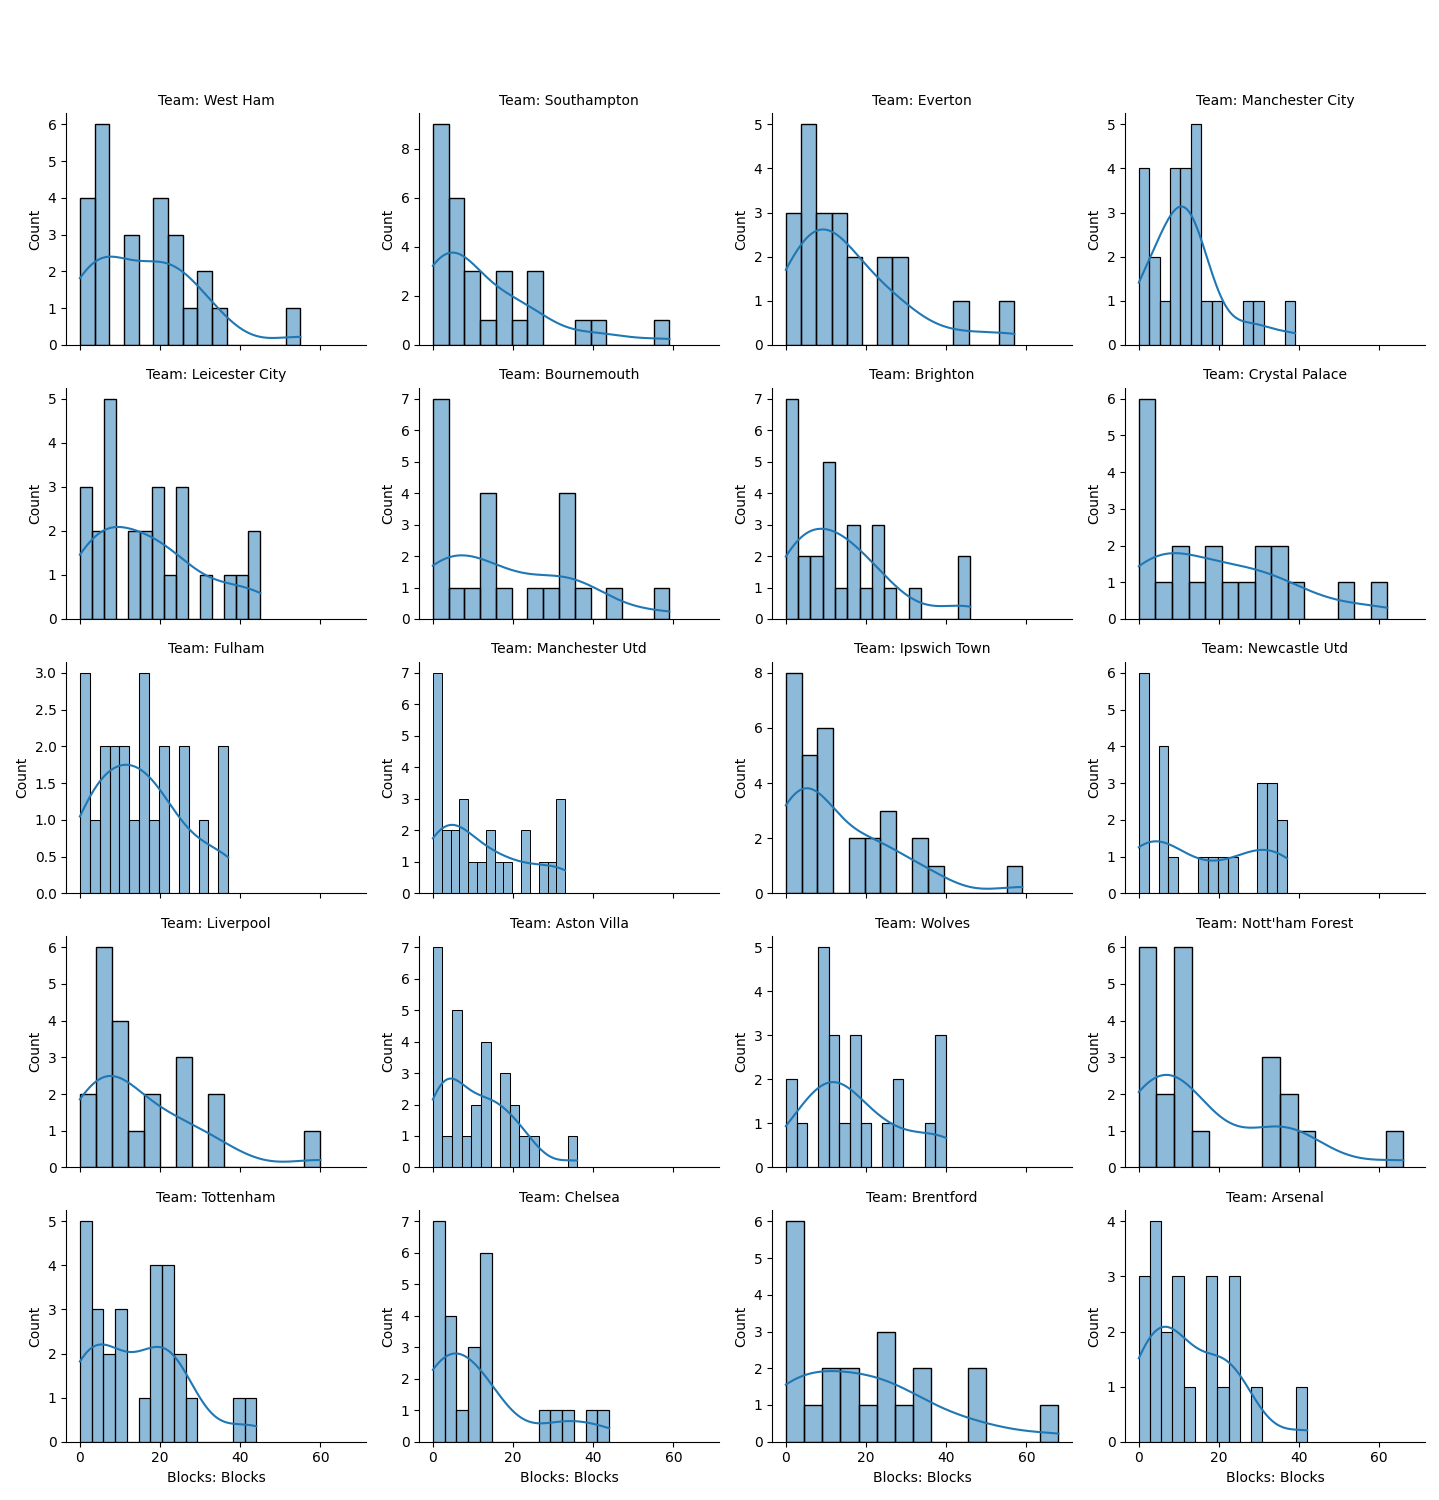
\includegraphics[width=300px]{Distribution_of_Blocks_Blocks_by_Team.png}
    \caption{File Distribution\_of\_Blocks\_Blocks\_by\_Team.png}
    \label{fig:p7}
\end{figure}
\clearpage
\textbf{Distribution\_of\_Performance\_goals\_by\_Team.png:}
Hình ảnh thể hiện dưới dạng ma trận lưới biểu đồ histogram gồm 24 biểu đồ con (4 hàng × 6 cột), mỗi biểu đồ đại diện cho một đội bóng khác nhau trong giải đấu.\\
Về hình thức:
\begin{itemize}
	\item Tiêu đề mỗi biểu đồ nằm phía trên cùng, ghi rõ tên đội (ví dụ: Team: Manchester City, Team: Arsenal).
	\item Trục hoành (X-axis) được gắn nhãn nhất quán là Performance: goals, thể hiện số bàn thắng.
	\item Trục tung (Y-axis) được đánh dấu là Count, biểu thị số lượng cầu thủ đạt mức bàn thắng tương ứng.
	\item Cột histogram màu xanh lam nhạt, kèm theo đường cong KDE màu xanh đậm nhằm biểu diễn mật độ xác suất phân bố bàn thắng của các cầu thủ trong từng đội.
\end{itemize}
Toàn bộ bố cục được sắp xếp đều đặn, đồng nhất về tỷ lệ và kiểu dáng, giúp dễ dàng so sánh sự phân bố bàn thắng giữa các đội bóng. Đây là kiểu trực quan hóa thường dùng trong báo cáo thống kê thể thao hoặc phân tích dữ liệu định lượng đa nhóm.
\\\\
\textbf{Distribution\_of\_Performance\_assists\_by\_Team.png:}
Hình ảnh này là một bố cục trực quan dạng lưới gồm 24 biểu đồ histogram nhỏ, mỗi biểu đồ đại diện cho một đội bóng khác nhau trong giải đấu. Về mặt hình thức, hình ảnh có các đặc điểm sau:
\begin{itemize}
	\item Cấu trúc lưới 6 cột × 4 hàng, giúp tổ chức biểu đồ một cách đều đặn và dễ theo dõi.
	\item Mỗi biểu đồ con có tiêu đề ở phía trên ghi rõ tên đội bóng, ví dụ: Team: Arsenal, Team: Manchester Utd, v.v.
	\item Trục hoành ở tất cả các biểu đồ được gán nhãn là Performance: goals, thể hiện số bàn thắng mà cầu thủ ghi được.
	\item Trục tung có nhãn là Count, biểu diễn số lượng cầu thủ tương ứng với từng mức bàn thắng.
	\item Trong mỗi biểu đồ, các cột histogram màu xanh lam nhạt biểu thị tần suất, đi kèm với một đường cong KDE màu xanh đậm, thể hiện mật độ phân bố xác suất.
	\item Kiểu dáng, tỷ lệ trục và bố cục biểu đồ được giữ nhất quán giữa các đội, tạo nên một tổng thể trực quan rõ ràng, dễ dàng để so sánh phân bố bàn thắng giữa các đội bóng.
\end{itemize}
Tổng thể, hình ảnh được trình bày theo phong cách khoa học và trực quan hóa dữ liệu chuẩn mực, phù hợp với các báo cáo học thuật hoặc phân tích thống kê định lượng trong lĩnh vực thể thao.
\\\\
\textbf{Distribution\_of\_Expected\_expected\_goals\_(xG)\_by\_Team.png:}
Hình ảnh này là một bố cục trực quan dạng lưới gồm 24 biểu đồ histogram nhỏ, mỗi biểu đồ đại diện cho một đội bóng khác nhau trong giải đấu. Về mặt hình thức, hình ảnh có các đặc điểm sau:
\begin{itemize}
	\item Cấu trúc lưới 6 cột × 4 hàng, giúp tổ chức biểu đồ một cách đều đặn và dễ theo dõi.
	\item Mỗi biểu đồ con có tiêu đề ở phía trên ghi rõ tên đội bóng, ví dụ: Team: Arsenal, Team: Manchester Utd, v.v.
	\item Trục hoành ở tất cả các biểu đồ được gán nhãn là Performance: expected\_goals (xG), thể hiện số bàn thắng kỳ vọng mà cầu thủ tạo ra.
	\item Trục tung có nhãn là Count, biểu diễn số lượng cầu thủ tương ứng với từng mức xG.
	\item Trong mỗi biểu đồ, các cột histogram màu xanh lam nhạt biểu thị tần suất, đi kèm với một đường cong KDE màu xanh đậm, thể hiện mật độ phân bố xác suất.
	\item Kiểu dáng, tỷ lệ trục và bố cục biểu đồ được giữ nhất quán giữa các đội, tạo nên một tổng thể trực quan rõ ràng, dễ dàng để so sánh phân bố xG giữa các đội bóng.
\end{itemize}
Tổng thể, hình ảnh được trình bày theo phong cách khoa học và trực quan hóa dữ liệu chuẩn mực, phù hợp với các báo cáo học thuật hoặc phân tích thống kê định lượng trong lĩnh vực thể thao.
\\\\
\textbf{Distribution\_of\_Tackles\_Tkl\_by\_Team.png:}
Hình ảnh là một bố cục trực quan gồm 24 biểu đồ nhỏ sắp xếp dạng lưới 6x4.
\begin{itemize}
	\item Tiêu đề từng biểu đồ con xác định rõ tên đội.
	\item Trục hoành là Performance: tackles\_tkl, phản ánh số pha tắc bóng của cầu thủ.
	\item Trục tung là Count, cho biết số cầu thủ đạt mức tắc bóng tương ứng.
	\item Histogram xanh lam nhạt và KDE xanh đậm tiếp tục là hình thức thể hiện chính.
	\item Sự nhất quán về tỷ lệ, màu sắc, bố cục và định dạng tiếp tục được duy trì.
\end{itemize}
Biểu đồ mang tính trực quan hóa mạnh cho các thống kê phòng ngự chủ động (tắc bóng) của các đội bóng.
\\\\
\textbf{Distribution\_of\_Challenges\_Att\_by\_Team.png:}
Hình ảnh trực quan này cũng gồm 24 biểu đồ nhỏ sắp xếp theo lưới 6x4, mỗi biểu đồ đại diện cho một đội bóng.
\begin{itemize}
	\item Tiêu đề mỗi biểu đồ con đều theo định dạng Team: [Tên đội].
	\item Trục hoành ghi là Performance: challenges\_att, biểu thị số lần tham gia tranh chấp bóng.
	\item Trục tung là Count, phản ánh số cầu thủ ứng với mỗi mức độ thử thách.
	\item Cột histogram xanh lam nhạt kết hợp đường KDE xanh đậm vẫn là phương pháp thể hiện chính.
	\item Tỷ lệ và khung hình giữ sự nhất quán tuyệt đối giữa các đội, giúp so sánh dễ dàng.
\end{itemize}
Hình ảnh mang tính trực quan hóa tốt cho các thống kê liên quan đến sức mạnh tranh chấp của từng đội.
\\\\
\textbf{Distribution\_of\_Blocks\_Blocks\_by\_Team.png:}
Hình ảnh này là một bố cục trực quan dạng lưới gồm 24 biểu đồ histogram nhỏ, mỗi biểu đồ đại diện cho một đội bóng khác nhau. Về mặt hình thức:
\begin{itemize}
	\item Cấu trúc dạng lưới 6 cột × 4 hàng được duy trì.
	\item Tiêu đề trên mỗi biểu đồ con thể hiện tên đội bóng, ví dụ: Team: Chelsea, Team: Leeds, v.v.
	\item Trục hoành được gán nhãn là Performance: blocks, thể hiện số lần cầu thủ thực hiện các pha cản phá.
	\item Trục tung là Count, cho biết số lượng cầu thủ tương ứng với từng mức blocks.
	\item Histogram màu xanh lam nhạt biểu thị tần suất, kết hợp đường KDE xanh đậm để thể hiện xu hướng phân bố.
	\item Bố cục, tỷ lệ và kiểu dáng đồng bộ, đảm bảo dễ dàng so sánh giữa các đội.
\end{itemize}
Tổng thể hình ảnh giữ phong cách chuyên nghiệp, có tính nhất quán cao, hỗ trợ hiệu quả cho việc phân tích phòng ngự giữa các đội.\\
\\\\
\textbf{best\_team\_summary.txt:}
\begin{figure}[h]
    \centering
    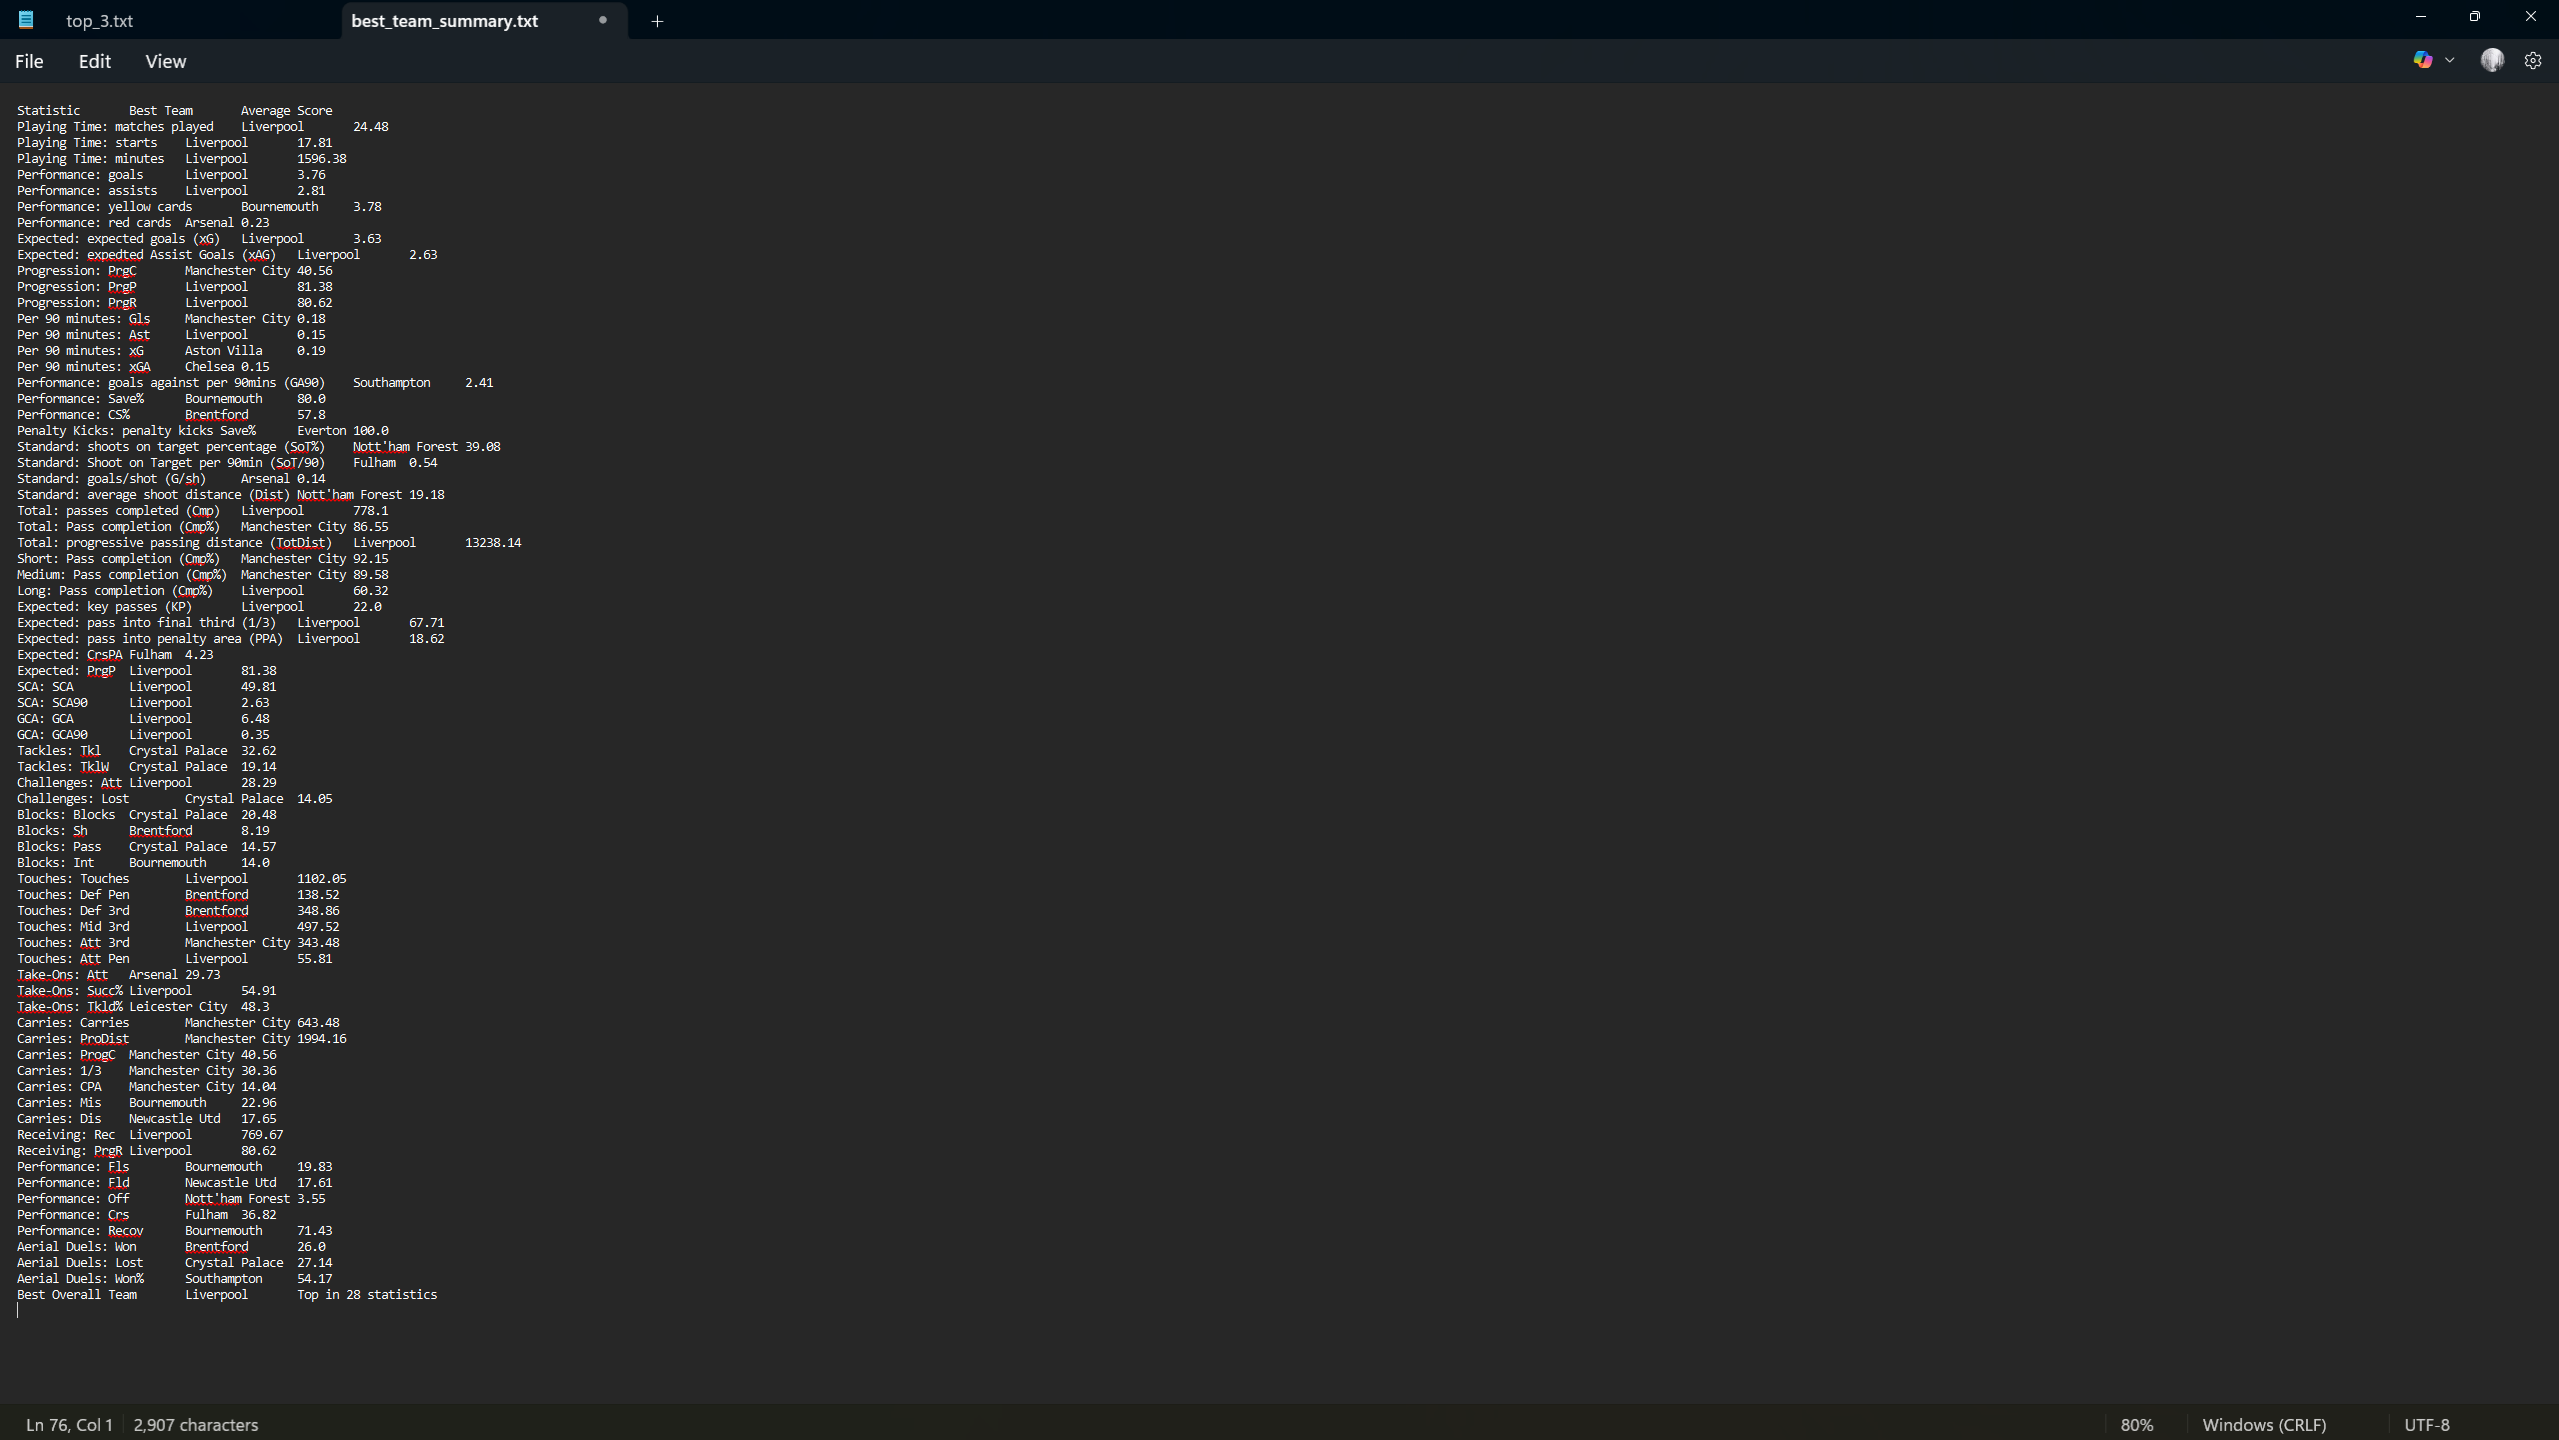
\includegraphics[width=300px]{best_team_summary.png}
    \caption{File best\_team\_summary.txt}
    \label{fig:p8}
\end{figure}
Tệp best\_team\_summary.txt này chứa một bản tóm tắt các số liệu thống kê về các đội bóng đá, có vẻ như là từ một giải đấu cụ thể. Dữ liệu được phân loại theo nhiều khía cạnh khác nhau của trận đấu như Tuổi (Age), Thời gian thi đấu (Playing Time), Hiệu suất (Performance), Chỉ số kỳ vọng (Expected), Khả năng phát triển bóng (Progression), Chỉ số tính trên 90 phút (Per 90 minutes), Thống kê về chuyền bóng (Total, Short, Medium, Long), Thống kê về phòng ngự (Tackles, Challenges, Blocks), Chạm bóng (Touches), Qua người (Take-Ons), Kéo bóng (Carries), Nhận bóng (Receiving), và Không chiến (Aerial Duels).   
\\
Đối với mỗi chỉ số thống kê, tệp liệt kê tên đội bóng dẫn đầu hạng mục đó cùng với giá trị trung bình (Avg) của đội đó cho chỉ số tương ứng. Ví dụ, Fulham có độ tuổi trung bình cao nhất (28.27), Liverpool dẫn đầu ở nhiều chỉ số tấn công như số trận đã đấu, số phút thi đấu, bàn thắng, kiến tạo, đường chuyền vào 1/3 cuối sân và vào vòng cấm, trong khi Manchester City nổi bật ở các chỉ số liên quan đến chuyền bóng và kéo bóng tịnh tiến. Các đội khác như Bournemouth, Arsenal, Crystal Palace, Brentford cũng dẫn đầu ở một số hạng mục cụ thể như thẻ vàng, thẻ đỏ, tắc bóng, chặn bóng.   
\\
Cuối cùng, tệp kết luận rằng Liverpool là "Đội bóng xuất sắc nhất toàn diện" (Best Overall Team) vì dẫn đầu trong 28 chỉ số thống kê. Đây cũng chính là câu trả lời cho câu hỏi: "Based on your analysis, which team do you think is performing the best in the 2024-2025 Premier League season?".

\subsection{Đánh giá}
Đoạn mã Problem2.py thể hiện nhiều ưu điểm nổi bật trong thiết kế và triển khai. Cấu trúc chương trình được tổ chức hợp lý với các hàm phân tách rõ ràng theo từng chức năng như tiền xử lý dữ liệu, phân tích thống kê mô tả, trực quan hóa và xuất kết quả, giúp nâng cao tính dễ hiểu và khả năng bảo trì. Mã sử dụng hiệu quả các thư viện như Pandas và Seaborn để xử lý dữ liệu và vẽ biểu đồ, từ đó hỗ trợ phân tích trực quan và toàn diện. Đáng chú ý, chương trình tích hợp đo lường thời gian chạy và bộ nhớ sử dụng thông qua thư viện tracemalloc, phản ánh rõ sự quan tâm đến hiệu suất thực thi. Cụ thể, thời gian thực thi được ghi nhận là 1.678 giây, với mức sử dụng bộ nhớ hiện tại là 6.66 MB và mức đỉnh là 42.91 MB, cho thấy chương trình vận hành hiệu quả và phù hợp với các hệ thống có giới hạn tài nguyên.
\\
Tuy nhiên, đoạn mã vẫn tồn tại một số hạn chế. Việc lựa chọn đội bóng xuất sắc nhất hiện chỉ dựa trên số lượng chỉ số mà đội đó dẫn đầu, trong khi chưa xem xét đến độ lớn của sự khác biệt hoặc tầm quan trọng tương đối giữa các chỉ số, điều này có thể dẫn đến kết quả thiếu khách quan trong một số trường hợp. Ngoài ra, kết quả đầu ra chủ yếu là các tệp văn bản và biểu đồ tĩnh, chưa hỗ trợ tương tác, điều này phần nào giới hạn trải nghiệm người dùng cuối và tiềm năng mở rộng ứng dụng lên các nền tảng trực tuyến hoặc hệ thống dashboard động.
}
\chapter{VẤN ĐỀ III}\
{
\section{Yêu cầu}
\begin{itemize}
	\item Use the K-means algorithm to classify players into groups based on their statistics.
	\item How many groups should the players be classified into? Why? Provide your comments on the results.
	\item Use PCA to reduce the data dimensions to 2, then plot a 2D cluster of the data points.
\end{itemize}
\section{Các bước tiến hành}
\begin{enumerate}
	\item \textbf{Tải và tiền xử lý dữ liệu:}
\begin{itemize}
  \item Đọc dữ liệu từ file \texttt{results.csv} (kết quả từ Vấn đề 1).
  \item Tách các cột định danh (Tên, Quốc tịch, Đội, Vị trí, Tuổi) và các cột chứa chỉ số thống kê.
  \item Chuyển đổi các cột thống kê sang dạng số, xử lý các giá trị không phải số bằng phương pháp \texttt{coerce}.
  \item Loại bỏ các cột chỉ chứa giá trị NaN.
  \item Xử lý các giá trị bị thiếu (NaN) bằng cách thay thế bằng trung vị (\texttt{median}) của cột tương ứng, sử dụng \texttt{SimpleImputer}.
  \item Chuẩn hóa dữ liệu bằng \texttt{StandardScaler} để đưa các chỉ số về cùng thang đo -- điều này quan trọng đối với K-means.
\end{itemize}

	\item \textbf{Xác định số cụm tối ưu (K):}
\begin{itemize}
  \item Sử dụng phương pháp Elbow để tính tổng bình phương sai số trong cụm (\texttt{inertia}) cho các giá trị $K$ từ 2 đến 15.
  \item Vẽ biểu đồ Elbow (\texttt{Inertia vs. K}) để xác định điểm ``khuỷu tay'', nơi tốc độ giảm inertia chậm lại đáng kể.
  \item Tính \texttt{Silhouette Score} cho các giá trị $K$ từ 2 đến 15 để đo lường sự phân tách giữa các cụm.
  \item Vẽ biểu đồ \texttt{Silhouette Score vs. K}. Giá trị $K$ cho Silhouette Score cao thường là lựa chọn tốt.
  \item Lưu các biểu đồ này thành file ảnh.
  \item Dựa trên cả hai biểu đồ để chọn số cụm tối ưu (ví dụ: $K=6$).
\end{itemize}

	\item \textbf{Áp dụng thuật toán K-means:}
\begin{itemize}
  \item Thực hiện phân cụm K-means với số cụm tối ưu đã chọn ($K = \texttt{optimal\_k}$) trên dữ liệu đã chuẩn hóa.
  \item Gán nhãn cụm cho từng cầu thủ.
  \item Thêm cột \texttt{Cluster} vào cả DataFrame gốc (\texttt{df}) và DataFrame đã chuẩn hóa (\texttt{df\_scaled}).
  \item Phân tích đặc điểm cụm bằng cách tính trung bình các chỉ số thống kê (chuẩn hóa và gốc) cho từng cụm.
\end{itemize}

	\item \textbf{Giảm chiều dữ liệu bằng PCA:}
\begin{itemize}
  \item Áp dụng PCA để giảm dữ liệu chuẩn hóa xuống còn 2 thành phần chính.
  \item Tạo DataFrame mới chứa 2 thành phần chính (PC1, PC2) và nhãn cụm tương ứng.
\end{itemize}

	\item \textbf{Trực quan hóa cụm 2D:}
\begin{itemize}
  \item Vẽ biểu đồ scatter plot 2D từ 2 thành phần PCA, tô màu điểm dữ liệu theo cụm K-means.
  \item Lưu biểu đồ thành file ảnh.
\end{itemize}
	\item \textbf{Lưu nhận xét và kết quả:}
\begin{itemize}
  \item Tạo file văn bản \texttt{comment\_P3.txt} ghi lại lý do chọn $K$, giải thích biểu đồ PCA và phân tích thành phần cụm.
\end{itemize}
\end{enumerate}
\section{Code thực tế và mô tả chi tiết}
\subsection{Hàm chính}
\begin{lstlisting}
def Problem_3():
    df_scaled, df, df_imputed = Load_and_Preprocess_Data()
    Determine_Optimal_K(df_scaled)
    optimal_k = 6
    print(f"\nBased on the Elbow method and Silhouette Score plots, choosing K = {optimal_k}.")
    cluster_labels = Apply_K_means(df_scaled, df, optimal_k, df_imputed)
    pca_clusters_df = Apply_PCA(df_scaled, cluster_labels)
    Plot_2D_Cluster(pca_clusters_df, optimal_k)

    #Create a file comments for the results
    with open(...) as f:
    	.....
\end{lstlisting}
Code được tổ chức thành các hàm trong file \texttt{Problem3.py}:

\begin{itemize}
  \item \texttt{Load\_and\_Preprocess\_Data()}: Tải dữ liệu, xử lý thiếu, chuẩn hóa. Trả về \texttt{df\_scaled}, \texttt{df}, \texttt{df\_imputed}.
  \item \texttt{Determine\_Optimal\_K(df\_scaled)}: Vẽ biểu đồ Elbow và Silhouette Score, lưu ảnh vào thư mục \texttt{P3\_RES}.
  \item \texttt{Apply\_K\_means(df\_scaled, df, optimal\_k, df\_imputed)}: Chạy K-means, gán nhãn cụm, in trung bình chỉ số.
  \item \texttt{Apply\_PCA(df\_scaled, cluster\_labels)}: Áp dụng PCA và trả về DataFrame chứa PC1, PC2, Cluster.
  \item \texttt{Plot\_2D\_Cluster(pca\_clusters\_df, optimal\_k)}: Vẽ biểu đồ 2D, lưu ảnh.
  \item \texttt{Problem\_3()}: Hàm chính điều phối toàn bộ quy trình, giả định chọn \texttt{optimal\_k = 6}, lưu kết quả và nhận xét vào thư mục \texttt{P3\_RES}.
\end{itemize}
\subsection{Chi tiết các thao tác}
\subsubsection{Hàm \texttt{Load\_and\_Preprocess\_Data()}}
\begin{lstlisting}
def Load_and_Preprocess_Data():
    Exclude_Cols = ['Name', 'Nation', 'Team', 'Position', 'Age']
    
    file_path = os.path.join('P1_RES', 'results.csv')
    df = pd.read_csv(file_path)
    # --- Preprocessing ---
    identifiers = df[Exclude_Cols]
    features = df.drop(columns=Exclude_Cols).apply(pd.to_numeric, errors='coerce')

    cols_all_nan = features.columns[features.isnull().all()]
    if not cols_all_nan.empty:
        features = features.drop(columns=cols_all_nan)

    imputer = SimpleImputer(strategy='median')
    scaler = StandardScaler()

    df_imputed = pd.DataFrame(imputer.fit_transform(features), columns=features.columns)
    df_scaled = pd.DataFrame(scaler.fit_transform(df_imputed), columns=df_imputed.columns)

    return df_scaled, df, df_imputed
\end{lstlisting}
Trong dòng 2, các cột định danh bao gồm \texttt{'Name'}, \texttt{'Nation'}, \texttt{'Team'}, \texttt{'Position'} và \texttt{'Age'} được liệt kê trong danh sách \texttt{Exclude\_Cols} nhằm loại trừ khỏi quá trình tiền xử lý dữ liệu. Ở dòng 4, đường dẫn tới tệp dữ liệu \texttt{'results.csv'} được xây dựng bằng cách kết hợp thư mục \texttt{'P1\_RES'} với tên tệp. Dữ liệu sau đó được đọc vào một \texttt{DataFrame} \texttt{df} bằng \texttt{pd.read\_csv()} (dòng 5).

Tiếp theo, dòng 7 tách các cột định danh khỏi \texttt{DataFrame} gốc để lưu trong biến \texttt{identifiers}, trong khi phần còn lại của dữ liệu – các đặc trưng số – được lưu vào \texttt{features}. Ở đây, \texttt{pd.to\_numeric(..., errors='coerce')} được sử dụng để chuyển đổi các giá trị không hợp lệ thành \texttt{NaN}, đảm bảo dữ liệu đầu vào cho các bước xử lý tiếp theo là dạng số.

Dòng 10-12 kiểm tra xem có cột nào chứa toàn giá trị thiếu (\texttt{NaN}) hay không. Nếu có, các cột này được loại bỏ khỏi \texttt{features} để tránh gây nhiễu trong quá trình huấn luyện mô hình.

Trong dòng 14, một đối tượng \texttt{SimpleImputer} được khởi tạo với chiến lược \texttt{'median'} để thay thế các giá trị thiếu bằng trung vị của từng cột, trong khi \texttt{StandardScaler} (dòng 15) được dùng để chuẩn hóa dữ liệu, đảm bảo mỗi đặc trưng có trung bình bằng 0 và độ lệch chuẩn bằng 1.

Sau đó, dữ liệu được điền khuyết bằng \texttt{imputer.fit\_transform()} và lưu vào \texttt{df\_imputed} (dòng 17), tiếp theo là quá trình chuẩn hóa bằng \texttt{scaler.fit\_transform()}, tạo thành \texttt{df\_scaled} (dòng 18).

Cuối cùng, hàm trả về ba đối tượng: \texttt{df\_scaled} (dữ liệu đã được chuẩn hóa), \texttt{df} (\texttt{DataFrame} gốc chưa xử lý), và \texttt{df\_imputed} (dữ liệu đã được điền khuyết nhưng chưa chuẩn hóa) (dòng 20).
\subsubsection{Hàm \texttt{Determine\_Optimal\_K(df\_scaled)}}
\begin{lstlisting}
def Determine_Optimal_K(df_scaled):
    inertia = []
    silhouette_scores = []
    kRange = range(2, 16)
    for k in kRange:
        kmeans = KMeans(n_clusters=k, random_state=42, n_init=10).fit(df_scaled)
        inertia.append(kmeans.inertia_)
        print(f"Inertia for k={k} calculated.", end=' ')
        if k > 1:
                try:
                    score = silhouette_score(df_scaled, kmeans.labels_)
                    silhouette_scores.append(score)
                    print(f"Silhouette Score: {score:.4f}")
                except ValueError as e:
                    print(f"  Could not calculate silhouette score for K={k}: {e}")
                    silhouette_scores.append(-1) # Append a placeholder if calculation fails

    plt.figure(figsize=(10, 6))
    plt.plot(kRange, inertia, 'o--')
    plt.xlabel('Number of Clusters (k)')
    plt.ylabel('Inertia')
    plt.title('Elbow Method for Optimal K')
    plt.xticks(list(kRange))
    plt.grid(True)
    plt.savefig(os.path.join('P3_RES', 'Elbow_Method_fo_Optimal_K.png'))
    plt.close()
    print(f'Elbow_Method_fo_Optimal_K.png is saved')

    valid_k_range_silhouette = list(kRange) # k_range already starts from 2
    plt.figure(figsize=(10, 6))
    plt.plot(valid_k_range_silhouette, silhouette_scores, marker='o')
    plt.title('Silhouette Score for Optimal K')
    plt.xlabel('Number of clusters (K)')
    plt.ylabel('Silhouette Score')
    plt.grid(True)
    plt.savefig(os.path.join('P3_RES', 'Silhouette_Score.png'))
    plt.close()
    print(f'Silhouette_Score.png is saved')
\end{lstlisting}
Hàm \texttt{Determine\_Optimal\_K} thực hiện quá trình xác định số lượng cụm tối ưu $K$ cho bài toán phân cụm sử dụng thuật toán \texttt{KMeans}, thông qua hai phương pháp phổ biến: phương pháp khuỷu tay (\textit{elbow method}) và điểm số \textit{silhouette}.

Đầu tiên, hai danh sách rỗng \texttt{inertia} và \texttt{silhouette\_scores} được khởi tạo để lưu các giá trị độ lệch tổng (\texttt{inertia}) và điểm \textit{silhouette} tương ứng với mỗi giá trị $K$ (dòng 2–3). Vòng lặp \texttt{for} từ dòng 4 xét dải giá trị $K$ từ 2 đến 15. Trong mỗi vòng lặp, một mô hình \texttt{KMeans} được huấn luyện với $K$ cụm (dòng 6), sau đó độ lệch tổng (\texttt{inertia\_}) được tính và lưu vào danh sách (dòng 7). Đây là chỉ số phản ánh mức độ chặt chẽ của các điểm dữ liệu trong mỗi cụm.

Từ dòng 9, nếu $K > 1$, thuật toán tiếp tục tính điểm \textit{silhouette} để đánh giá chất lượng phân cụm bằng cách đo mức độ tương đồng của điểm dữ liệu với cụm của chính nó so với cụm gần nhất kế tiếp. Giá trị này được tính bằng \texttt{silhouette\_score()} (dòng 12) và lưu vào danh sách \texttt{silhouette\_scores}. Nếu quá trình tính toán gặp lỗi (ví dụ khi cụm chỉ có một điểm), ngoại lệ được xử lý (dòng 14–15) và một giá trị mặc định -1 được thêm vào danh sách như một phần tử đại diện (dòng 16).

Tiếp theo, hàm tạo biểu đồ khuỷu tay (dòng 18–27) bằng cách vẽ đồ thị tương quan giữa $K$ và \texttt{inertia}. Mục tiêu là tìm điểm gãy (\textit{elbow point}) – tại đó việc gia tăng số cụm không mang lại lợi ích rõ rệt về mặt giảm độ lệch tổng. Hình ảnh được lưu dưới tên \texttt{'Elbow\_Method\_fo\_Optimal\_K.png'} (dòng 25) trong thư mục \texttt{'P3\_RES'}.

Sau đó, từ dòng 29–38, hàm tiếp tục trực quan hóa điểm \textit{silhouette} tương ứng với các giá trị $K$, nhằm xác định giá trị $K$ tối ưu dựa trên chất lượng phân cụm. Biểu đồ được lưu lại với tên \texttt{'Silhouette\_Score.png'} (dòng 37).
\\
\subsubsection{Thao tác chọn K:} Đây là một thao tác ở bên ngoài ta đưa giá trị K vào thông qua quan sát đồ thị để tìm điểm khuỷu tay cũng như quan sát cực trị của đồ thị hình chiếu để đưa ra số K tốt nhất.
\\
\subsubsection{Hàm \texttt{Apply\_K\_means(df\_scaled, df, optimal\_k, df\_imputed)}}
\begin{lstlisting}
def Apply_K_means(df_scaled, df, optimal_k, df_imputed):
    kmeans = KMeans(n_clusters=optimal_k, random_state=42, n_init=10)
    cluster_labels = kmeans.fit_predict(df_scaled)

    df['Cluster'] = cluster_labels
    df_scaled['Cluster'] = cluster_labels

    print(f"K-means clustering complete with k={optimal_k}.")

    # --- Cluster Analysis ---
    print("\n--- Cluster Analysis ---")
    print("\nMean (scaled features) per cluster:")
    print(df_scaled.groupby('Cluster').mean())

    df_imputed['Cluster'] = cluster_labels
    print("\nMean (original features) per cluster:")

    stats = [
    'Performance: goals', 
    'Performance: assists', 
    'Tackles: TklW',
    'Blocks: Int',
    'Performance: Save%'
    ]
    available_stats = [s for s in stats if s in df_imputed.columns]
    print(df_imputed.groupby('Cluster')[available_stats].mean())
    print("-" * 50)
    return cluster_labels
\end{lstlisting}
Tại dòng 2, một đối tượng \texttt{KMeans} được khởi tạo với số cụm bằng \texttt{optimal\_k}, tham số \texttt{random\_state} được cố định để đảm bảo tính lặp lại của kết quả, và \texttt{n\_init=10} nhằm chạy thuật toán nhiều lần để tránh nghiệm xấu. Sau đó, mô hình được huấn luyện và gán nhãn cụm cho mỗi mẫu dữ liệu thông qua phương thức \texttt{fit\_predict()} (dòng 3), kết quả được lưu vào \texttt{cluster\_labels}.

Các nhãn cụm được thêm vào cả \texttt{DataFrame} gốc \texttt{df} và dữ liệu chuẩn hóa \texttt{df\_scaled} dưới dạng cột mới \texttt{'Cluster'} (dòng 5–6). Sau đó, chương trình in ra thông báo xác nhận hoàn tất quá trình phân cụm (dòng 8).

Phần phân tích cụm bắt đầu từ dòng 11, với việc hiển thị trung bình của các đặc trưng đã chuẩn hóa (scaled features) theo từng cụm thông qua \texttt{groupby('Cluster').mean()} trên \texttt{df\_scaled} (dòng 13). Tiếp theo, các nhãn cụm cũng được thêm vào \texttt{DataFrame} \texttt{df\_imputed} (dòng 15) để phục vụ phân tích các đặc trưng nguyên gốc (trước chuẩn hóa).

Tại dòng 18–25, một danh sách các đặc trưng thống kê quan trọng như số bàn thắng, kiến tạo, tắc bóng, cản phá và tỷ lệ cứu thua được định nghĩa trong biến \texttt{stats}. Tuy nhiên, vì không phải tất cả các đặc trưng này luôn tồn tại trong dữ liệu, danh sách \texttt{available\_stats} được lọc để chỉ giữ lại các cột thực sự tồn tại trong \texttt{df\_imputed}. Sau đó, trung bình của các đặc trưng này theo cụm được in ra (dòng 26).
Cuối cùng, hàm trả về mảng \texttt{cluster\_labels} chứa nhãn cụm tương ứng với từng hàng dữ liệu (dòng285). Hàm này là bước cuối cùng trong chu trình phân cụm, cung cấp cả đầu ra định lượng (nhãn cụm) và phân tích mô tả (đặc trưng trung bình theo cụm).
\\
\subsubsection{Hàm \texttt{Apply\_PCA(df\_scaled, cluster\_labels)}}
\begin{lstlisting}
def Apply_PCA(df_scaled, cluster_labels):
    print("Applying PCA...")
    pca = PCA(n_components=2)
    components = pca.fit_transform(df_scaled.drop(columns='Cluster'))

    pca_clusters_df = pd.DataFrame(components, columns=['PC1', 'PC2'])
    pca_clusters_df['Cluster'] = cluster_labels

    print(f"PCA complete. Explained variance: {pca.explained_variance_ratio_.sum():.4f}")

    return pca_clusters_df
\end{lstlisting}
Dòng 2 in thông báo bắt đầu quá trình PCA. Sau đó, một đối tượng \texttt{PCA} với số thành phần chính là 2 (\texttt{n\_components=2}) được khởi tạo (dòng 3). Việc lựa chọn hai thành phần chính cho phép biểu diễn dữ liệu trong không gian hai chiều (PC1 và PC2), phù hợp cho mục đích trực quan hóa.

Tại dòng 4, dữ liệu chuẩn hóa \texttt{df\_scaled} được loại bỏ cột \texttt{'Cluster'} nhằm tránh ảnh hưởng đến quá trình giảm chiều, sau đó được biến đổi bằng phương pháp PCA để thu được hai thành phần chính. Kết quả được lưu trong biến \texttt{components}.

Ở dòng 6, một \texttt{DataFrame} mới tên là \texttt{pca\_clusters\_df} được tạo, chứa hai thành phần chính (PC1, PC2), và nhãn cụm \texttt{cluster\_labels} được thêm vào như một cột mới nhằm phục vụ việc phân biệt cụm trên đồ thị.

Dòng 9 in ra tổng phương sai được giải thích bởi hai thành phần chính đầu tiên thông qua phương thức \texttt{explained\_variance\_ratio\_.sum()}, cho biết mức độ mà hai chiều này có thể tái hiện thông tin từ dữ liệu ban đầu.

Cuối cùng, hàm trả về \texttt{DataFrame} \texttt{pca\_clusters\_df} (dòng 11), là đầu vào lý tưởng cho bước trực quan hóa kết quả phân cụm trong không gian hai chiều.
\\
\subsubsection{Hàm \texttt{Plot\_2D\_Cluster(pca\_clusters\_df, optimal\_k)}}
\begin{lstlisting}
def Plot_2D_Cluster(pca_clusters_df, optimal_k):
    plt.figure(figsize=(12, 8))
    sns.scatterplot(
        x='PC1', y='PC2', hue='Cluster', 
        palette=sns.color_palette('viridis', n_colors=optimal_k),
        data=pca_clusters_df, legend='full', alpha=0.7
    )
    plt.title(f'PCA of Clusters (k={optimal_k})')
    plt.grid(True)
    plt.savefig(os.path.join('P3_RES', f'PCA_of_Clusters_k={optimal_k}.png'))
    plt.close()
    print(f'PCA_of_Clusters_k={optimal_k}.png is saved')
\end{lstlisting}
Ở dòng 2, một khung hình đồ thị với kích thước lớn (12x8) được khởi tạo để đảm bảo hiển thị rõ ràng các cụm. Từ dòng 3 đến dòng 7, hàm \texttt{sns.scatterplot()} từ thư viện Seaborn được sử dụng để vẽ biểu đồ phân tán (\texttt{scatter plot}), trong đó:

Trục hoành (x) và trục tung (y) lần lượt là hai thành phần chính \texttt{PC1} và \texttt{PC2} từ \texttt{DataFrame} \texttt{pca\_clusters\_df}.

Mỗi điểm dữ liệu được tô màu theo cụm (\texttt{hue='Cluster'}), sử dụng bảng màu \texttt{viridis} với số màu tương ứng với \texttt{optimal\_k}.

Tham số \texttt{alpha=0.7} tạo độ trong suốt nhẹ giúp quan sát sự chồng lấp dễ dàng hơn, và \texttt{legend='full'} cho phép hiển thị đầy đủ các nhãn cụm trong chú thích.

Tiêu đề biểu đồ được gán theo giá trị của \texttt{K} (dòng 8), và lưới biểu đồ được bật để hỗ trợ theo dõi tọa độ (dòng 9). Đồ thị được lưu vào thư mục \texttt{'P3\_RES'} với tên chứa số cụm \texttt{K} (dòng 10), và sau đó đóng lại bằng \texttt{plt.close()} để giải phóng bộ nhớ (dòng 11). Cuối cùng, một thông báo xác nhận được in ra (dòng 12).
\section{Kết quả và đánh giá}
Chương trình tạo ra các file sau trong thư mục \texttt{P3\_RES}:
\begin{itemize}
  \item \texttt{Elbow\_Method\_fo\_Optimal\_K.png}: Biểu đồ Elbow cho thấy điểm khuỷu tay.
  \item \texttt{Silhouette\_Score.png}: Biểu đồ Silhouette Score để đánh giá chất lượng phân cụm.
  \item \texttt{PCA\_of\_Clusters\_k=6.png}: Scatter plot 2D trực quan hóa các cụm.
  \item \texttt{comment\_P3.txt}: Ghi chú chọn $K=6$, phân tích biểu đồ PCA, thống kê cụm (ví dụ: vị trí phổ biến nhất trong mỗi cụm).
\end{itemize}
\subsection{Kết quả:}
\begin{figure}[h]
    \centering
    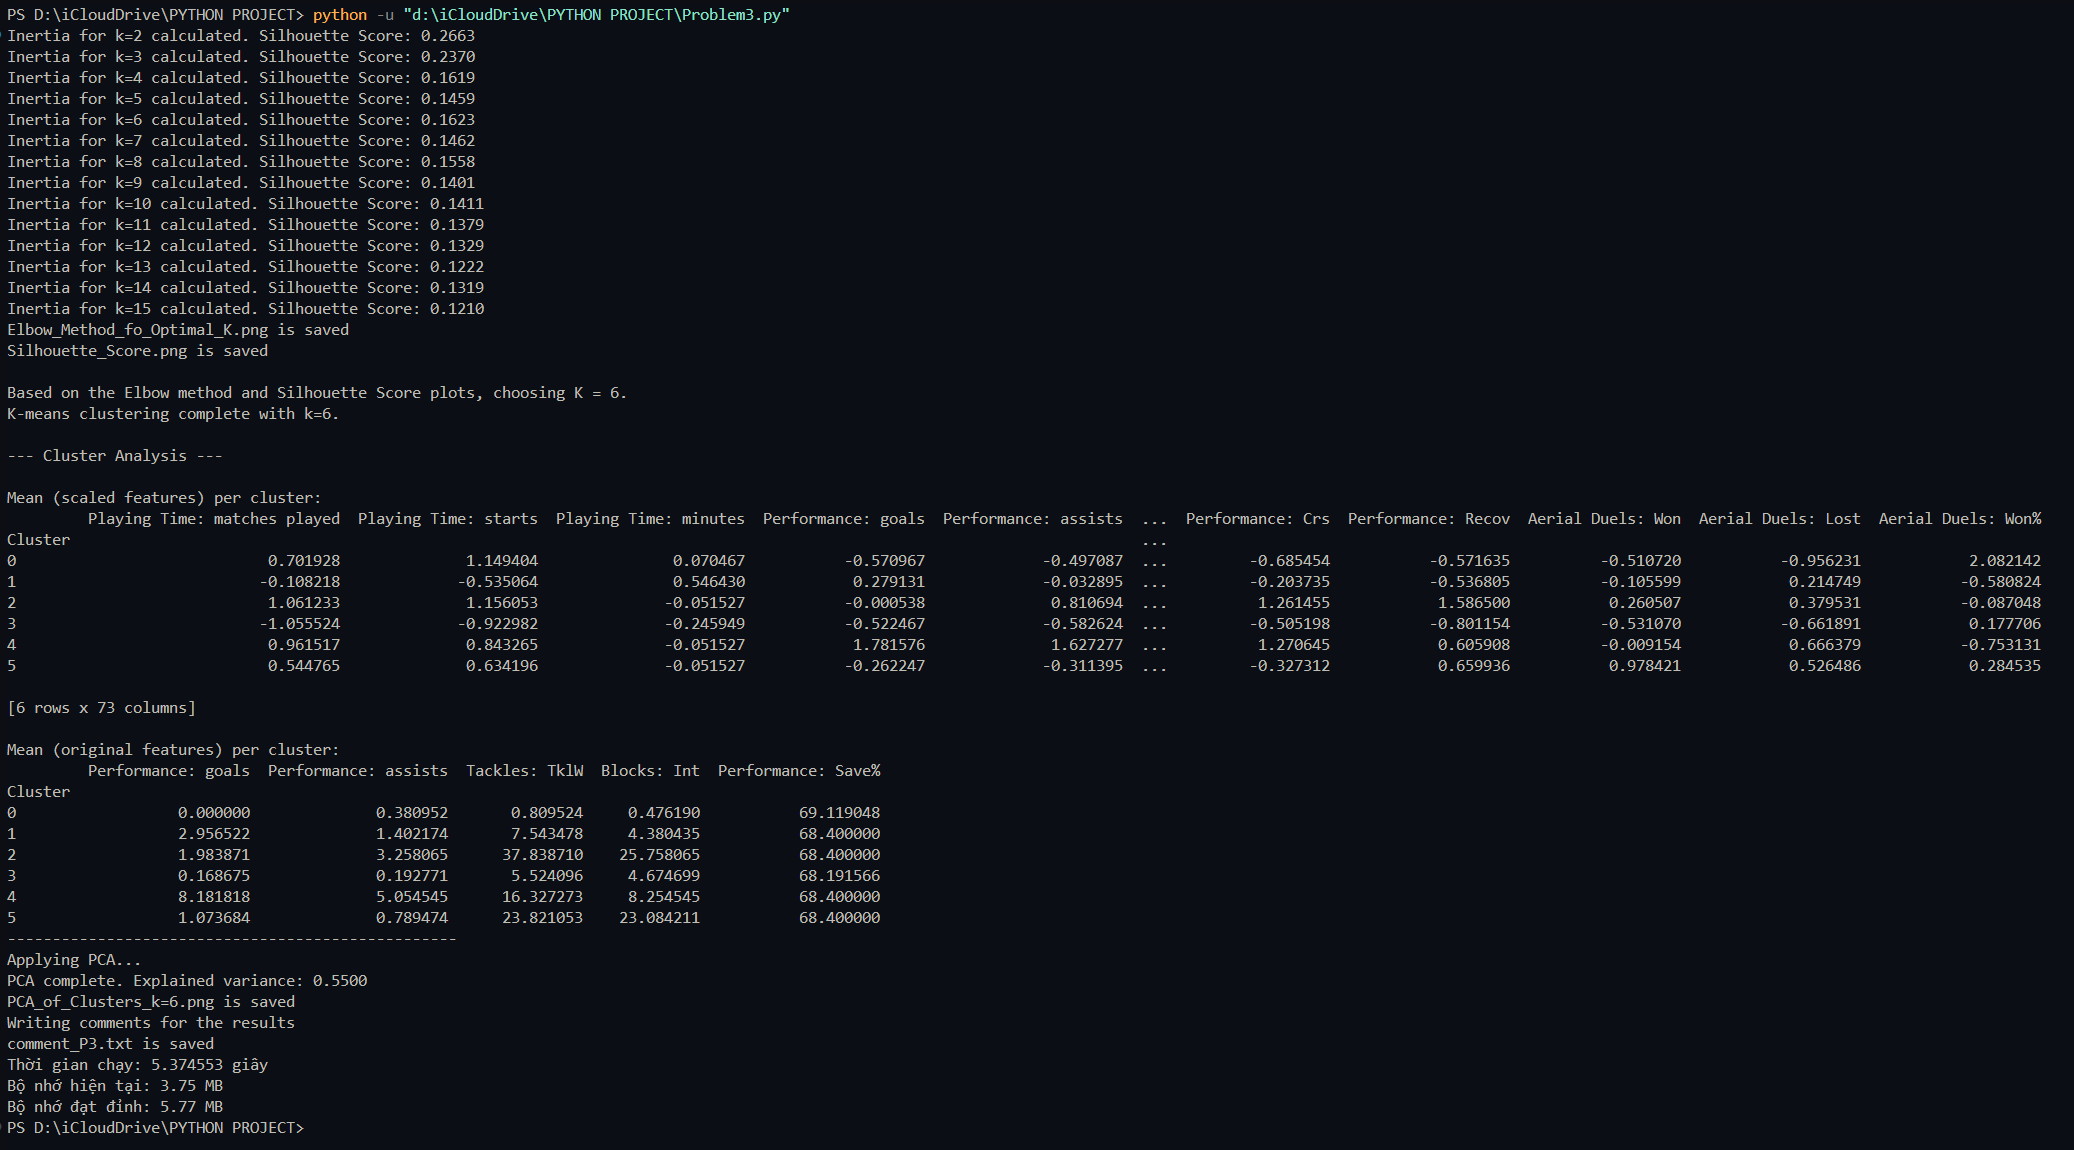
\includegraphics[width=300px]{Terminal_3.png}
    \caption{Terminal sau khi thực hiện chương tring Problem3.py}
    \label{fig:term3}
\end{figure}
Dựa trên ảnh chụp màn hình terminal, đây là một đoạn văn học thuật mô tả về quá trình thực thi tập lệnh, tập trung vào khía cạnh thời gian chạy và mức độ sử dụng bộ nhớ:

Đoạn output terminal này ghi lại quá trình thực thi một tập lệnh phân tích dữ liệu (có thể là bằng ngôn ngữ Python), thể hiện các bước xử lý chính bao gồm phân tích cụm (clustering) và giảm chiều dữ liệu (dimensionality reduction). Về mặt thời gian chạy (runtime), quá trình này bao gồm các giai đoạn tính toán lặp lại cho thuật toán k-means trên một loạt các giá trị của k nhằm xác định số lượng cụm tối ưu, được chứng minh qua việc tính toán các chỉ số Inertia và Silhouette Score. Tiếp theo là giai đoạn phân tích cụm chi tiết và áp dụng Phân tích Thành phần Chính (PCA), một kỹ thuật yêu cầu các phép toán ma trận chuyên sâu. Thời gian thực thi tổng cộng được báo cáo là khoảng 5.32 giây (với đơn vị có thể tùy chỉnh hoặc bị viết tắt). Các thông báo về thời gian thực thi riêng cho PCA và k-means là 3.75 ms cho mỗi phần, tuy nhiên con số này có vẻ thấp bất thường so với tổng thời gian và quy mô các phép tính, có thể chỉ đại diện cho một phần rất nhỏ hoặc cụ thể của các quy trình đó. Quá trình cũng bao gồm việc lưu trữ các kết quả trung gian và cuối cùng vào các tệp tin, đóng góp vào tổng thời gian chạy thông qua các thao tác vào/ra dữ liệu (I/O).

Về khía cạnh bộ nhớ (memory), mặc dù output không cung cấp thông tin cụ thể về việc sử dụng RAM, ta có thể suy luận về yêu cầu bộ nhớ dựa trên các tác vụ được thực hiện. Tải dữ liệu ban đầu vào bộ nhớ là bước cơ bản. Các thuật toán như k-means và PCA, đặc biệt khi xử lý các tập dữ liệu lớn với nhiều mẫu và thuộc tính, yêu cầu đáng kể không gian bộ nhớ để lưu trữ ma trận dữ liệu, ma trận hiệp phương sai (trong PCA), các tâm cụm (centroids), và kết quả phân cụm của từng điểm dữ liệu. Mức độ sử dụng bộ nhớ sẽ tăng tỷ lệ thuận với kích thước dữ liệu đầu vào và độ phức tạp tính toán của các thuật toán được triển khai. Việc lưu các đồ thị và kết quả vào tệp cũng tạm thời sử dụng bộ nhớ đệm cho các thao tác ghi dữ liệu.
\\
\begin{figure}[h]
    \centering
    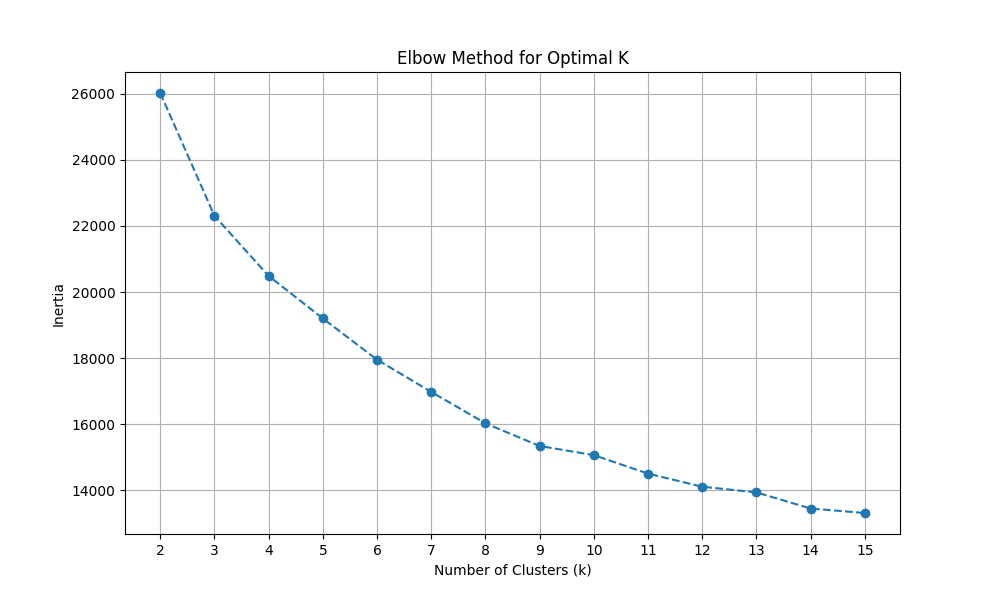
\includegraphics[width=300px]{Elbow_Method_fo_Optimal_K.png}
    \caption{File: Elbow\_Method\_fo\_Optimal\_K.png}
    \label{fig:Elbow}
\end{figure}
Biểu đồ Elbow\_Method\_fo\_Optimal\_K là một đồ thị đường (line plot) hai chiều, được sử dụng để minh họa "Phương pháp Khuỷu tay" (Elbow Method), một kỹ thuật heuristic phổ biến dùng để xác định số lượng cụm tối ưu (k) trong phân tích cụm, điển hình là thuật toán k-means. Trục hoành của biểu đồ biểu diễn số lượng cụm (k), một biến rời rạc được đánh số nguyên từ 2 đến 15. Trục tung biểu diễn giá trị Inertia, hay còn gọi là Tổng bình phương khoảng cách bên trong cụm (Within-cluster sum of squares - WCSS), một thước đo mức độ chặt chẽ của các cụm. Mỗi điểm dữ liệu trên đồ thị (được đánh dấu bằng hình tròn màu xanh) tương ứng với giá trị Inertia được tính toán cho một số lượng cụm k cụ thể. Các điểm này được nối với nhau bằng một đường nét đứt, tạo thành một đường cong thể hiện sự thay đổi của Inertia khi số lượng cụm tăng lên. Hình thức trình bày này cho phép người phân tích quan sát xu hướng giảm của Inertia khi k tăng và tìm điểm "uốn cong" hoặc "khuỷu tay" trên đường cong, nơi tốc độ giảm của Inertia chậm lại đáng kể, gợi ý về một giá trị k tiềm năng là tối ưu. Biểu đồ cũng được trang bị lưới (grid) để hỗ trợ việc đọc và ước lượng giá trị trên cả hai trục.
\\
\begin{figure}[h]
    \centering
    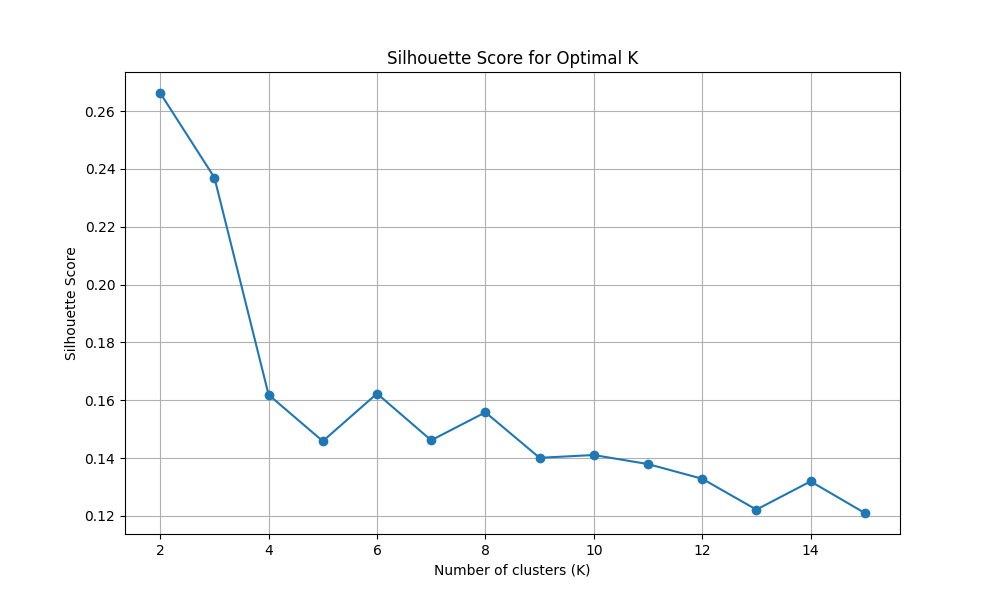
\includegraphics[width=300px]{Silhouette_Score.png}
    \caption{File: Silhouette\_Score.png}
    \label{fig:Silhouette}
\end{figure}
Biểu đồ Silhouette\_Score là một đồ thị đường (line plot) hai chiều, được sử dụng để trực quan hóa chỉ số \texttt{Silhouette Score} cho các số lượng cụm (\texttt{k}) khác nhau, hỗ trợ quá trình xác định số lượng cụm tối ưu trong phân tích cụm. Trục hoành của biểu đồ biểu diễn số lượng cụm (\texttt{K}), là một biến rời rạc với các giá trị nguyên từ 2 đến 15. Trục tung biểu diễn giá trị trung bình của \texttt{Silhouette Score}, một thước đo sự gắn kết (\textit{cohesion}) và sự tách biệt (\textit{separation}) của các cụm, với giá trị nằm trong khoảng \([-1, 1]\).

Mỗi điểm dữ liệu trên đồ thị (được đánh dấu bằng hình tròn màu xanh) thể hiện giá trị \texttt{Silhouette Score} tương ứng với một giá trị \texttt{k}. Các điểm này được nối với nhau bằng một đường liền nét, tạo thành một đường cong minh họa sự biến thiên của \texttt{Silhouette Score} khi số lượng cụm thay đổi. Hình thức biểu diễn này cho phép người phân tích dễ dàng xác định giá trị \texttt{k} nào mang lại chỉ số \texttt{Silhouette Score} cao nhất, vì giá trị cao hơn thường được coi là dấu hiệu của cấu trúc phân cụm tốt hơn.

Biểu đồ cũng bao gồm một lưới (\texttt{grid}) để tạo điều kiện thuận lợi cho việc đọc và diễn giải các giá trị trên cả hai trục.
\\
\begin{figure}[h]
    \centering
    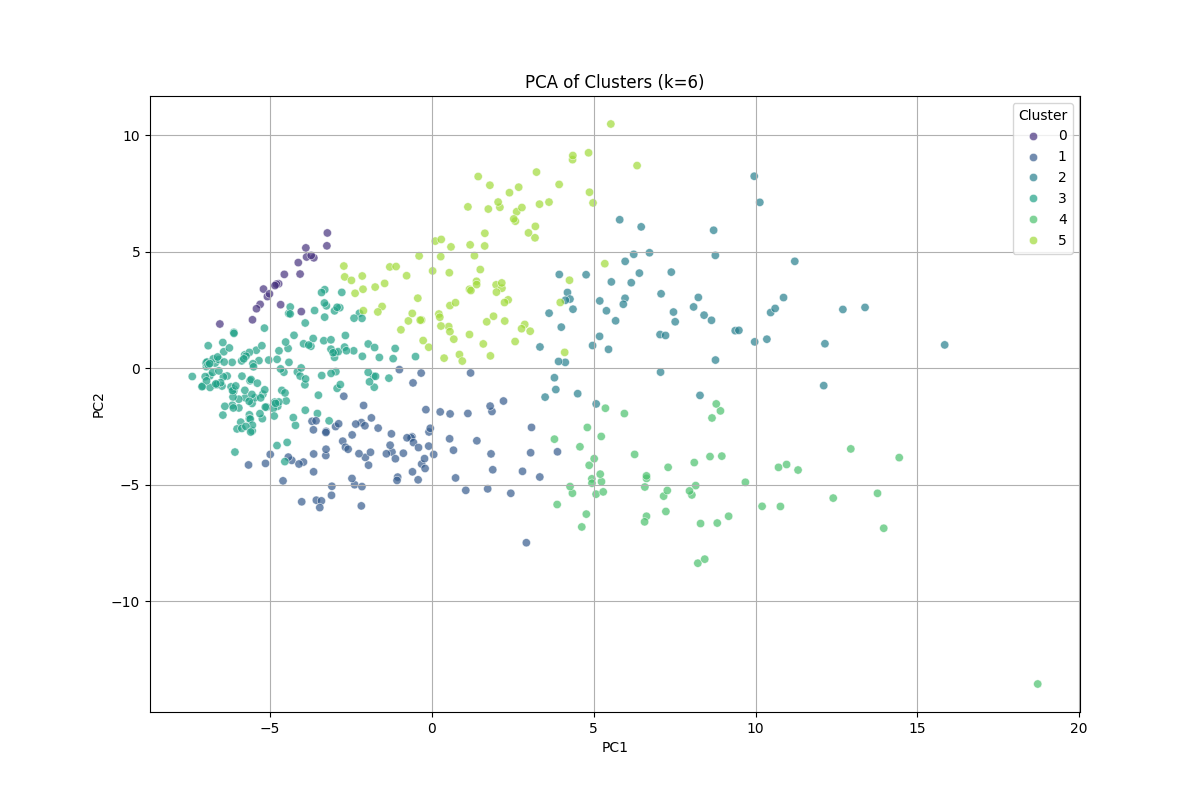
\includegraphics[width=300px]{PCA_of_Clusters_k=6.png}
    \caption{File: PCA\_of\_Clusters\_k=6.png}
    \label{fig:PCA}
\end{figure}
Biểu đồ PCA\_of\_Clusters\_k=6 là một đồ thị phân tán (scatter plot) hai chiều, được xây dựng để trực quan hóa kết quả của một thuật toán phân cụm (cụ thể với số lượng cụm k=6) sau khi dữ liệu gốc đã được giảm chiều bằng phương pháp Phân tích Thành phần Chính (PCA). Trục hoành của biểu đồ biểu diễn giá trị của Thành phần Chính thứ nhất (PC1), trong khi trục tung biểu diễn giá trị của Thành phần Chính thứ hai (PC2). Hai thành phần này là các biến liên tục, đại diện cho hai hướng có phương sai lớn nhất trong tập dữ liệu ban đầu sau khi áp dụng phép biến đổi PCA. Mỗi điểm trên đồ thị tương ứng với một đơn vị dữ liệu hoặc mẫu từ tập dữ liệu gốc. Đặc điểm hình thức nổi bật của biểu đồ là việc sử dụng màu sắc để mã hóa thông tin phân cụm: mỗi điểm dữ liệu được gán một màu sắc khác nhau tùy thuộc vào cụm mà nó được chỉ định bởi thuật toán phân cụm. Chú giải (legend) ở góc trên bên phải cung cấp ánh xạ giữa màu sắc và chỉ số của từng cụm (từ 0 đến 5). Hình thức trình bày này cho phép người xem đánh giá mức độ tách biệt và cấu trúc của các cụm trong không gian hai chiều được chiếu từ dữ liệu gốc, giúp hình dung hiệu quả của quá trình phân cụm. Biểu đồ cũng bao gồm lưới (grid) để hỗ trợ việc định vị và so sánh các điểm dữ liệu.
\\
\textbf{Nội dung file comment\_P3.txt:}\\
\text{1. Number of Clusters (K)}
Dựa trên hai phương pháp phân tích phổ biến là \textbf{Elbow Method} và \textbf{Silhouette Score}, số cụm tối ưu được lựa chọn là \textbf{K=6}. Cụ thể:
\begin{itemize}
  \item Biểu đồ Elbow cho thấy độ giảm của \textit{Within-Cluster Sum of Squares (WCSS)} bắt đầu chậm lại tại $K=6$, hàm ý rằng việc tăng thêm số cụm sau đó không mang lại cải thiện đáng kể.
  \item Biểu đồ Silhouette Score cho thấy giá trị đỉnh hoặc cao tại $K=6$, cho thấy mức độ tách biệt giữa các cụm là hợp lý.
  \item Điều này phù hợp với hiểu biết thực tế về vai trò của các cầu thủ bóng đá, thường được chia thành các nhóm đặc trưng như \textit{Thủ môn (GK), Hậu vệ (DF), Tiền vệ (MF), Tiền đạo (FW)}.
\end{itemize}

\text{2. PCA and Clustering Plot}
\begin{itemize}
  \item PCA được áp dụng để giảm 74 đặc trưng ban đầu xuống còn 2 thành phần chính (principal components) phục vụ cho việc trực quan hóa dữ liệu.
  \item Biểu đồ phân tán 2D mô tả sự phân bố của các cầu thủ trên hai trục PC1 và PC2, với màu sắc thể hiện cụm tương ứng từ kết quả K-means.
\end{itemize}

\textbf{Ý nghĩa biểu đồ:}
\begin{itemize}
  \item Quan sát sự tách biệt giữa các cụm: Nếu các cụm phân bố rõ ràng, điều này thể hiện mô hình phân cụm hoạt động tốt.
  \item Mối liên hệ với vị trí thi đấu: Ta có thể xác nhận độ phù hợp bằng cách kiểm tra giá trị trong cột \texttt{Position} của các cầu thủ trong từng cụm. Ví dụ: một cụm có thể gần như toàn bộ là \texttt{GK} do thống kê đặc trưng riêng biệt, trong khi các cụm khác chia theo tuyến phòng ngự, tiền vệ, và tấn công.
  \item Mật độ và độ phân tán của các điểm trong từng cụm phản ánh mức độ tương đồng của các cầu thủ trong cụm đó.
\end{itemize}

\text{3. Ví dụ Thành phần Các Cụm}

\begin{itemize}
  \item \textbf{Cluster 0} \\
  Tổng số cầu thủ: 21 \\
  Vị trí chính: GK (21)

  \item \textbf{Cluster 1} \\
  Tổng số cầu thủ: 92 \\
  Vị trí chính: \\
  \quad FW: 33, FW,MF: 32, MF,FW: 14, MF: 4, FW,DF: 3

  \item \textbf{Cluster 2} \\
  Tổng số cầu thủ: 62 \\
  Vị trí chính: \\
  \quad DF: 27, MF: 24, MF,FW: 5, FW,MF: 2, MF,DF: 2

  \item \textbf{Cluster 3} \\
  Tổng số cầu thủ: 166 \\
  Vị trí chính: \\
  \quad DF: 77, MF: 30, GK: 18, FW: 11, DF,MF: 10

  \item \textbf{Cluster 4} \\
  Tổng số cầu thủ: 55 \\
  Vị trí chính: \\
  \quad FW: 27, FW,MF: 15, MF,FW: 9, MF: 4

  \item \textbf{Cluster 5} \\
  Tổng số cầu thủ: 95 \\
  Vị trí chính: \\
  \quad DF: 56, MF: 28, DF,MF: 5, MF,DF: 4, DF,FW: 1
 \end{itemize}
\subsection{Đánh giá:}
\begin{itemize}
  \item \textbf{Ưu điểm:}
  \begin{itemize}
    \item Phân cụm không giám sát hiệu quả, phát hiện nhóm cầu thủ tương đồng mà không cần gán nhãn.
    \item Trực quan hóa tốt bằng PCA giúp hiểu rõ cấu trúc dữ liệu.
    \item Tiền xử lý đầy đủ giúp cải thiện hiệu suất mô hình.
    \item Kết hợp cả Elbow và Silhouette để chọn $K$ đáng tin cậy hơn.
  \end{itemize}
  \item \textbf{Nhược điểm:}
  \begin{itemize}
    \item Nhạy với lựa chọn $K$ và chuẩn hóa đầu vào.
    \item PCA giảm chiều gây mất một phần thông tin.
    \item Khó giải thích cụm do đặc thù dữ liệu bóng đá phức tạp.
    \item K-means giả định cụm hình cầu và kích thước tương đương – không phải lúc nào cũng đúng.
  \end{itemize}
\end{itemize}

Tổng kết: Kết hợp K-means và PCA cung cấp cái nhìn sơ bộ hữu ích về cấu trúc dữ liệu, nhưng cần bổ sung kiến thức chuyên môn để diễn giải sâu hơn.
}
\chapter{VẤN ĐỀ IV}
{
\section{Yêu cầu}
\begin{itemize}
	\item Collect player transfer values for the 2024-2025 season from https://www.footballtransfers.com. Note that only collect for the players whose playing time is greater than 900 minutes.
	\item Propose a method for estimating player values. How do you select feature and model?
\end{itemize}
\section{Các bước tiến hành}
\subsection{Yêu cầu 1}
\begin{enumerate}
	\item Nhập vào dữ liệu vào từ file results.csv từ Vấn đề I. Lọc những cầu thủ có thời gian thi đấu trên 900 phút.
	\item Cập nhật dữ liệu Tranfer values (Giá trị chuyển nhượng từ web https://www.footballtransfers.com/us/players/uk-premier-league/.)
	\item Lưu lại kết quả.
\end{enumerate}
\subsection{Yêu cầu 2}
\begin{enumerate}
	\item Lựa chọn phương pháp ước tính giá trị chuyển nhượng cầu thủ.
	\item Lựa chọn những trường dữ liệu có ảnh hưởng lớn đến giá trị cầu thủ.
	\item Triển khai code bằng ngôn ngữ python.
	\item Kiểm thử và đánh giá khả năng hoạt động của chương trình.
\end{enumerate}
\section{Xử lý yêu cầu 1}
\subsection{Code thực tế và mô tả chi tiết}
\subsubsection{Hàm chính}
\begin{lstlisting}
def Task_1():
    filtered_df = get_data()
    player_dic = update_data(filtered_df)
    save_result(filtered_df, player_dic)
\end{lstlisting}
\textbf{Hàm xử lý thực hiện theo từng phần đã mô tả ở mục các bước tiến hành:}
\begin{itemize}
	\item Hàm get\_data() Có chức năng lấy dữ liệu từ file results.csv đã lưu ở Vấn đề 1. Trả về DataFrame là các cầu thủ có thời gian thi đấu trên 900 phút.
	\item update\_data(filtered\_df) Có chức năng cập nhật giá trị chuyển nhượng của các cầu thủ từ web https://www.footballtransfers.com/us/players/uk-premier-league/. Trả về dictionary cầu thủ đó player\_dic gồm các cầu thủ có thời gian thi đấu trên 900 phút.
	\item save\_result(filtered\_df, player\_dic) Có chức năng đưa những giá trị vào DataFrame cầu thủ theo player\_dic, cố định trong DataFrame và lưu lại kết quả.
\end{itemize}
\subsubsection{Chi tiết các thao tác}
\textbf{Hàm get\_data():}\\
\begin{lstlisting}
def get_data():
    df = pd.read_csv('results.csv')

    # Clean the 'Playing Time: minutes' column
    df['Playing Time: minutes'] = df['Playing Time: minutes'].str.replace(',', '').astype(int)

    # Filter players with more than 900 minutes
    filtered_df = df[df['Playing Time: minutes'] > 900]

    return filtered_df
\end{lstlisting}
Dòng 2 đọc dữ liệu từ file results.csv rồi cố định vào DataFrame df. Dòng 5 Xử lý dữ liệu thời gian thi đấu về chuẩn format kiểu int (xử lý để dấu ',' ở trong số). Dòng 8 lọc những hàng mà có thời gian thi đấu lớn hơn 900 theo như yêu cầu cảu đề bài. Lưu vào DataFrame mới filtered\_df. Dòng 10 trẩ về filtered\_df.
\\\\
\textbf{Hàm update\_data(filtered\_df):}\\
\begin{lstlisting}
def update_data(filtered_df):
    player_dic = {}
    for name in filtered_df['Name']:
        player_dic[name] = ''

    driver = webdriver.Chrome()

    url = 'https://www.footballtransfers.com/us/players/uk-premier-league/'
    driver.get(url)
    names = []
    prices = []
    while True:
        page_source = driver.page_source
        soup = BeautifulSoup(page_source, 'html.parser')
        
        table = soup.find('table', class_='table table-hover no-cursor table-striped leaguetable mvp-table similar-players-table mb-0')
        
        name_tags = table.find_all('div', class_='text')
        price_tags = table.find_all('span', class_='player-tag')
        
        for n in name_tags:
            a_tag = n.find('a')
            if a_tag:
                names.append(a_tag.get('title'))

        for p in price_tags:
            prices.append(p.text.strip())
        
        try:
            next_button = driver.find_element(By.CLASS_NAME, 'pagination_next_button')
            next_button.click()
        except:
            break

    driver.quit()
    
    for i in range(len(names)):
        if names[i] in player_dic:
            player_dic[names[i]] = prices[i]
            
    return player_dic
\end{lstlisting}
Hàm \texttt{update\_data(filtered\_df)} (dòng 1) được thiết kế để tự động thu thập và cập nhật giá trị chuyển nhượng của các cầu thủ bóng đá từ trang web \url{footballtransfers.com}, giới hạn trong khuôn khổ giải Ngoại hạng Anh. Đầu tiên, hàm khởi tạo một từ điển rỗng \texttt{player\_dic = \{\}} (dòng 2), nơi sẽ lưu trữ tên cầu thủ làm khóa và giá trị chuyển nhượng làm giá trị. Sau đó, nó duyệt qua từng cầu thủ trong cột \texttt{'Name'} của \texttt{DataFrame} đầu vào và gán cho họ giá trị rỗng ban đầu \texttt{player\_dic[name] = ''} (dòng 4), nhằm chuẩn bị cho quá trình cập nhật dữ liệu thực tế.

Trình duyệt tự động Chrome được khởi tạo thông qua \texttt{webdriver.Chrome()} (dòng 6) và điều hướng tới URL chứa dữ liệu cầu thủ bằng lệnh \texttt{driver.get(url)} (dòng 9). Hai danh sách rỗng \texttt{names = []} và \texttt{prices = []} (dòng 10–11) được khai báo để lần lượt lưu trữ tên và giá trị cầu thủ được trích xuất từ trang web. Một vòng lặp \texttt{while True:} (dòng 12) được sử dụng để liên tục duyệt qua các trang kết quả cho đến khi không còn trang kế tiếp.

Trong mỗi vòng lặp, mã HTML hiện tại của trang được lấy thông qua \texttt{driver.page\_source} (dòng 13) và được phân tích bằng thư viện \texttt{BeautifulSoup} \texttt{soup = BeautifulSoup(...)} (dòng 14). Bảng chứa dữ liệu cầu thủ được tìm bằng cách sử dụng class cụ thể \texttt{table = soup.find(...)} (dòng 16). Sau đó, các thẻ chứa tên cầu thủ (\texttt{name\_tags = table.find\_all(...)}, dòng 18) và giá trị chuyển nhượng (\texttt{price\_tags = table.find\_all(...)}, dòng 19) được thu thập.

Hàm tiếp tục phân tích từng thẻ \texttt{div} chứa tên cầu thủ. Nếu thẻ con \texttt{<a>} tồn tại thì tên cầu thủ sẽ được lấy qua thuộc tính \texttt{title} và thêm vào danh sách \texttt{names.append(...)} (dòng 24). Tương tự, giá trị chuyển nhượng được lấy bằng \texttt{p.text.strip()} (dòng 27) và lưu vào danh sách \texttt{prices}.

Để tiếp tục sang trang tiếp theo, chương trình tìm nút phân trang thông qua \texttt{driver.find\_element(...)} (dòng 30) và gọi phương thức \texttt{.click()} để chuyển trang. Nếu không còn nút này (bị lỗi), vòng lặp sẽ kết thúc với khối \texttt{except:} (dòng 32). Trình duyệt sau đó được đóng lại bằng \texttt{driver.quit()} (dòng 35), nhằm giải phóng tài nguyên hệ thống.

Cuối cùng, hàm duyệt qua toàn bộ danh sách tên cầu thủ đã thu thập, và nếu tên đó tồn tại trong từ điển ban đầu, thì sẽ cập nhật giá trị chuyển nhượng bằng \texttt{player\_dic[names[i]] = prices[i]} (dòng 39). Kết quả cuối cùng là một từ điển ánh xạ tên cầu thủ với giá trị chuyển nhượng tương ứng, được trả về qua lệnh \texttt{return player\_dic} (dòng 41).
\\\\
\textbf{Hàm save\_result(filtered\_df, player\_dic):}\\
\begin{lstlisting}
def save_result(filtered_df, player_dic):
    filtered_df['Transfer values'] = player_dic.values()
    filtered_df.to_csv('MoreThan900mins.csv', index=False, encoding='utf-8-sig')
\end{lstlisting}
Hàm \texttt{save\_result(filtered\_df, player\_dic)} (dòng 1) thực hiện việc lưu trữ kết quả sau khi đã cập nhật giá trị chuyển nhượng cầu thủ. Cụ thể, nó thêm một cột mới \texttt{'Transfer values'} vào \texttt{DataFrame} từ các giá trị trong \texttt{player\_dic} (dòng 2).  Với cấu hình không ghi chỉ số dòng và sử dụng mã hóa \texttt{'utf-8-sig'} để đảm bảo khả năng đọc file tốt hơn (dòng 3).

\subsection{Kết quả và Đánh giá}
\subsubsection{Kết quả}
\begin{figure}[h]
    \centering
    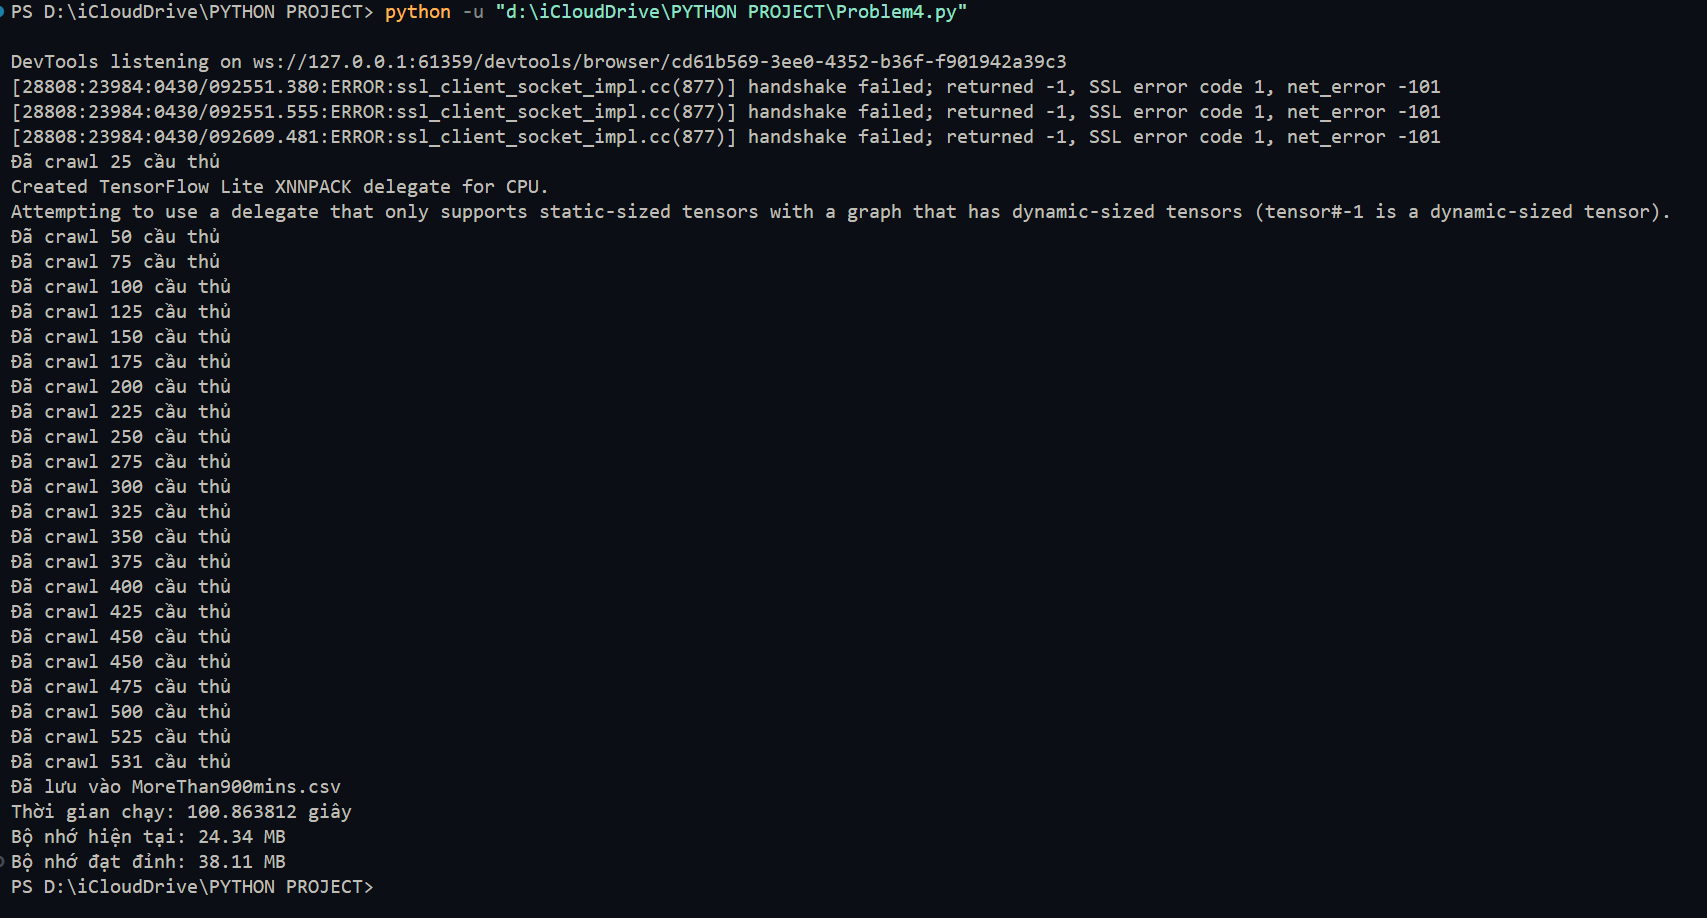
\includegraphics[width=300px]{Terminal_4.png}
    \caption{Terminal sau khi thực hiện function Task\_1}
    \label{fig:res2}
\end{figure}
Về phương diện thời gian, quá trình thực thi script, được biểu thị bằng việc crawl 531 mục ("câu thủ") và lưu dữ liệu vào file CSV, hoàn thành trong khoảng 100.86 giây. Khoảng thời gian này cung cấp một chỉ số định lượng về tốc độ xử lý của chương trình đối với khối lượng công việc đã thực hiện, cho phép đánh giá hiệu quả thuật toán hoặc tác vụ I/O liên quan đến việc crawl và lưu trữ. Về phương diện dung lượng bộ nhớ, xuất terminal cung cấp cả bộ nhớ hiện tại đang sử dụng (24.34 MB) và bộ nhớ đạt đỉnh trong suốt quá trình chạy (38.11 MB). Sự chênh lệch giữa hai giá trị này chỉ ra rằng chương trình có những giai đoạn yêu cầu lượng bộ nhớ tạm thời cao hơn mức sử dụng ổn định. Mức sử dụng bộ nhớ đạt đỉnh 38.11 MB tương đối thấp, cho thấy chương trình này có hiệu quả về mặt tài nguyên bộ nhớ đối với quy mô dữ liệu và tác vụ được thực hiện trong lần chạy cụ thể này, không đòi hỏi lượng RAM lớn. Tổng hợp lại, các chỉ số thời gian và dung lượng bộ nhớ từ terminal cung cấp dữ liệu định lượng quan trọng để phân tích hiệu suất của script, cho phép đánh giá tính hiệu quả và khả năng mở rộng của chương trình.\\\\
\begin{figure}[h]
    \centering
    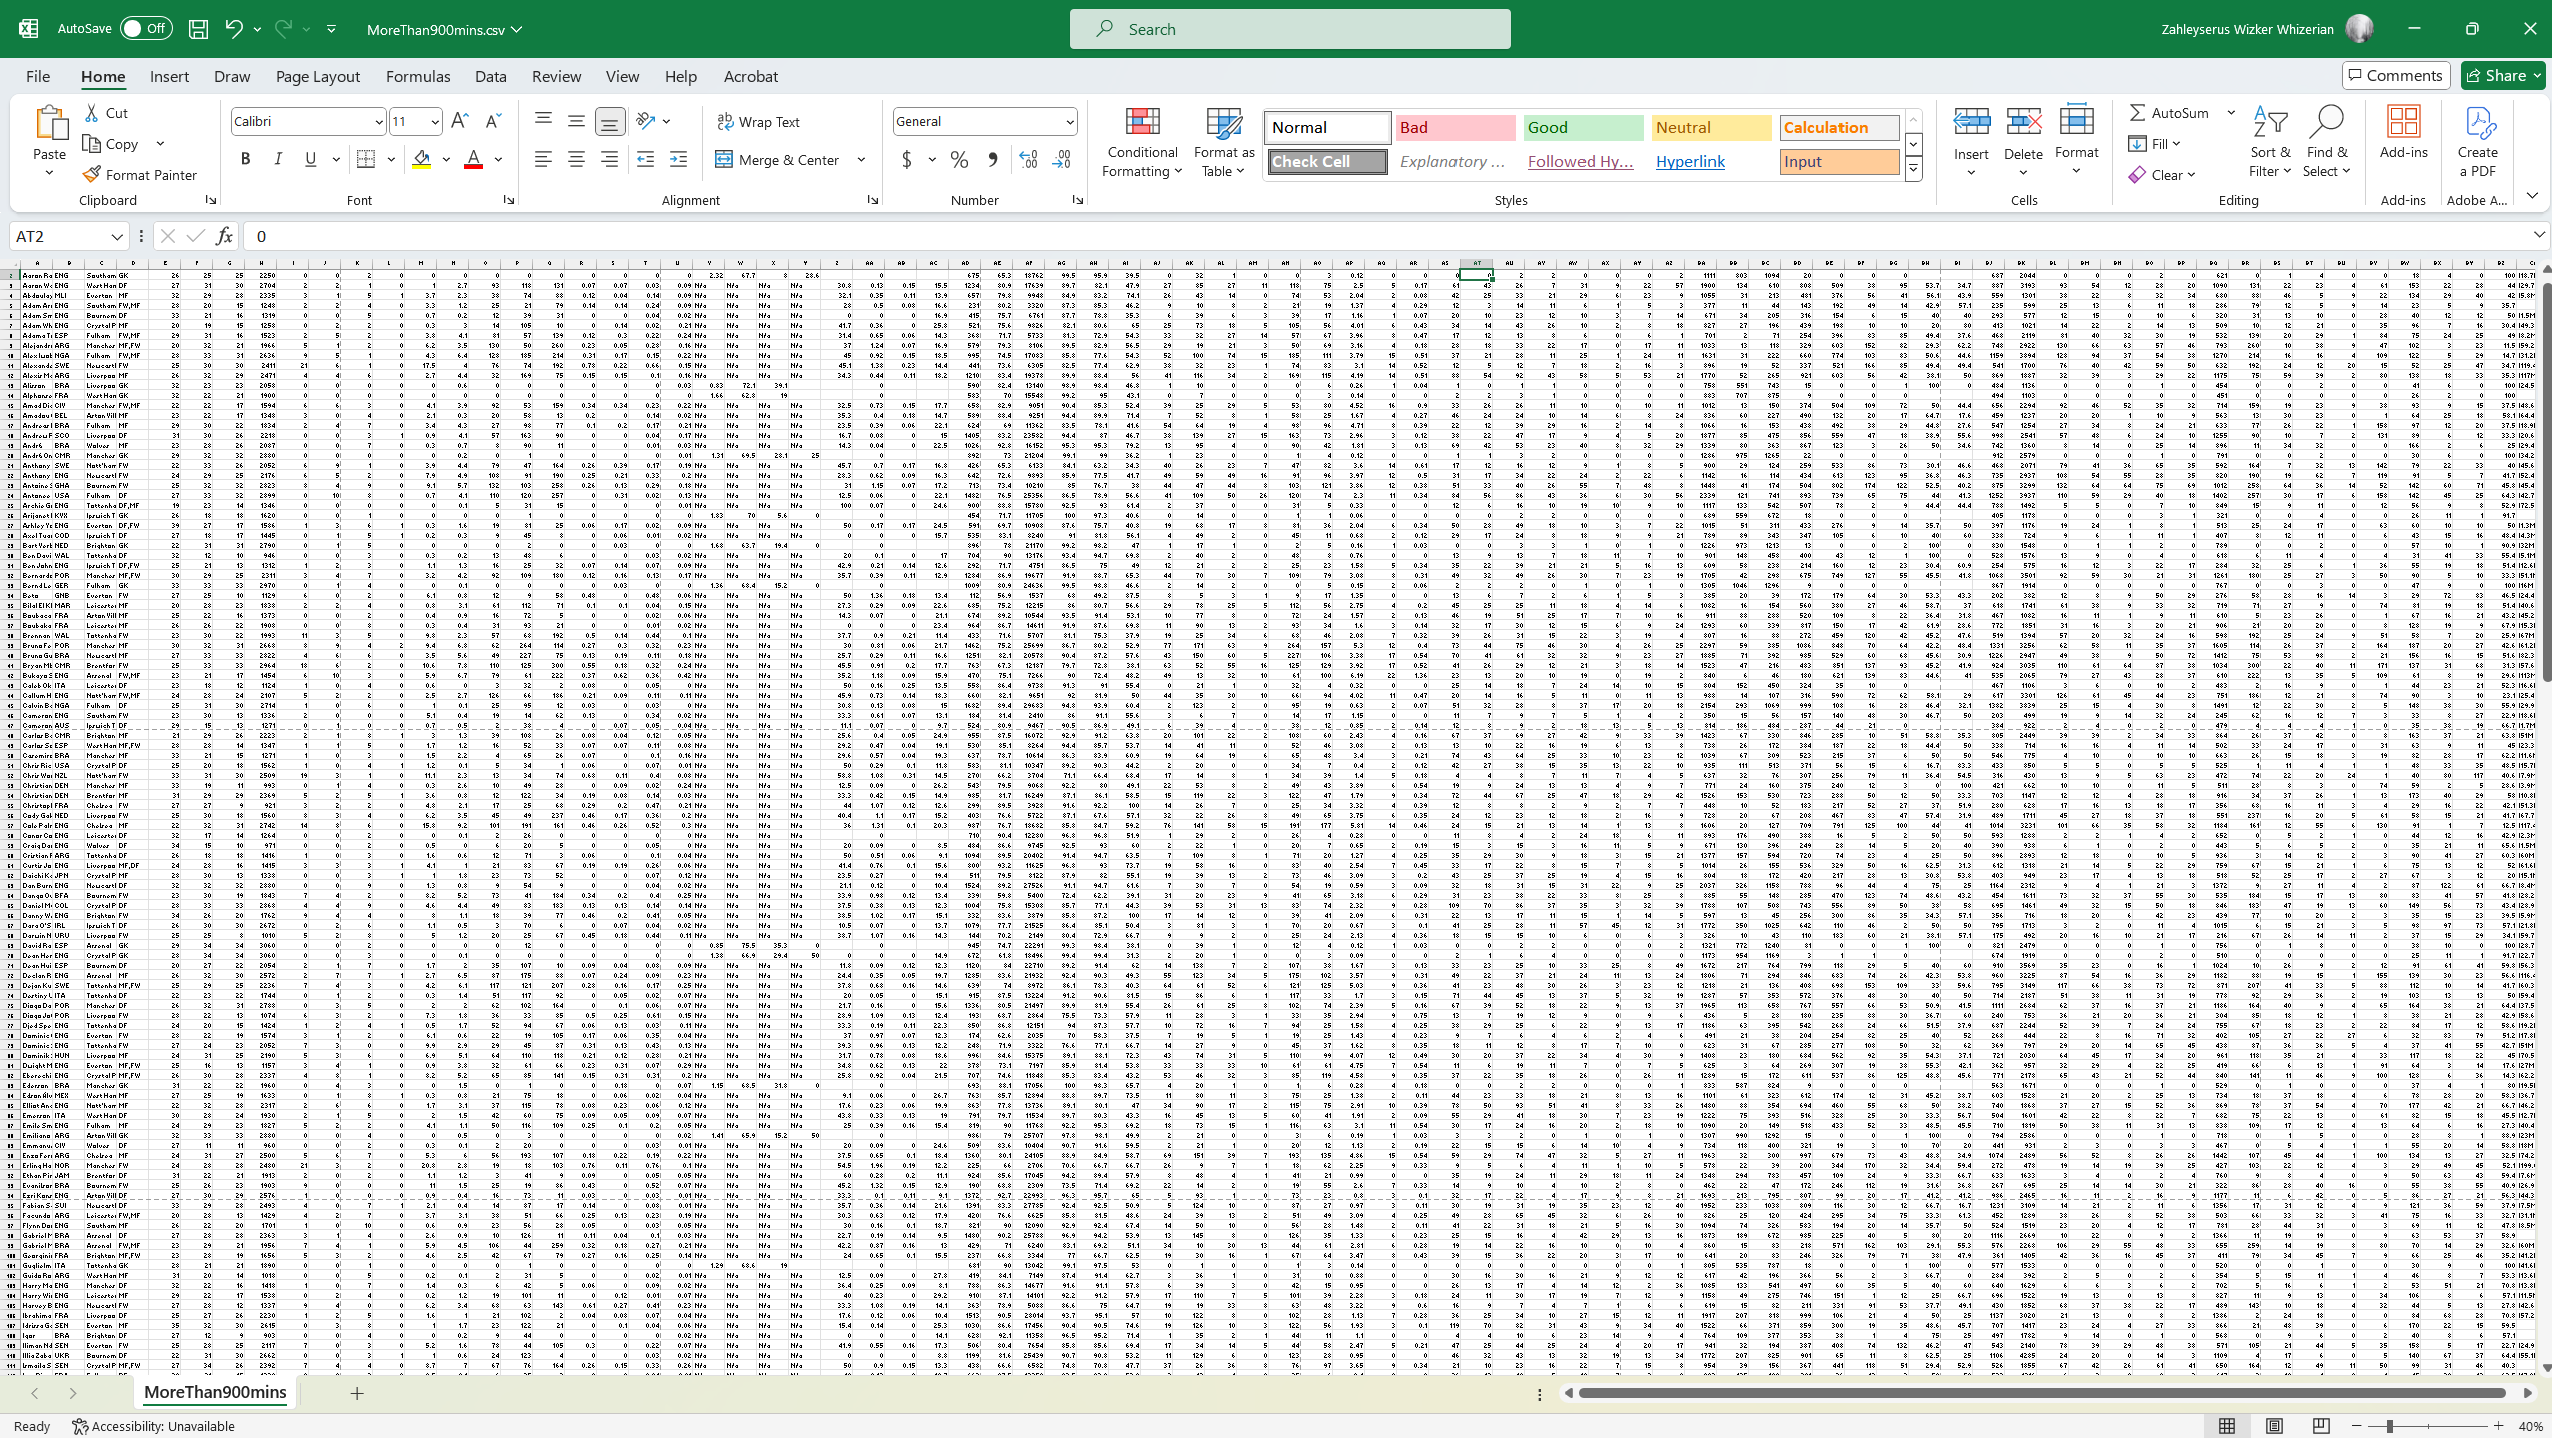
\includegraphics[width=350px]{P4_RES.png}
    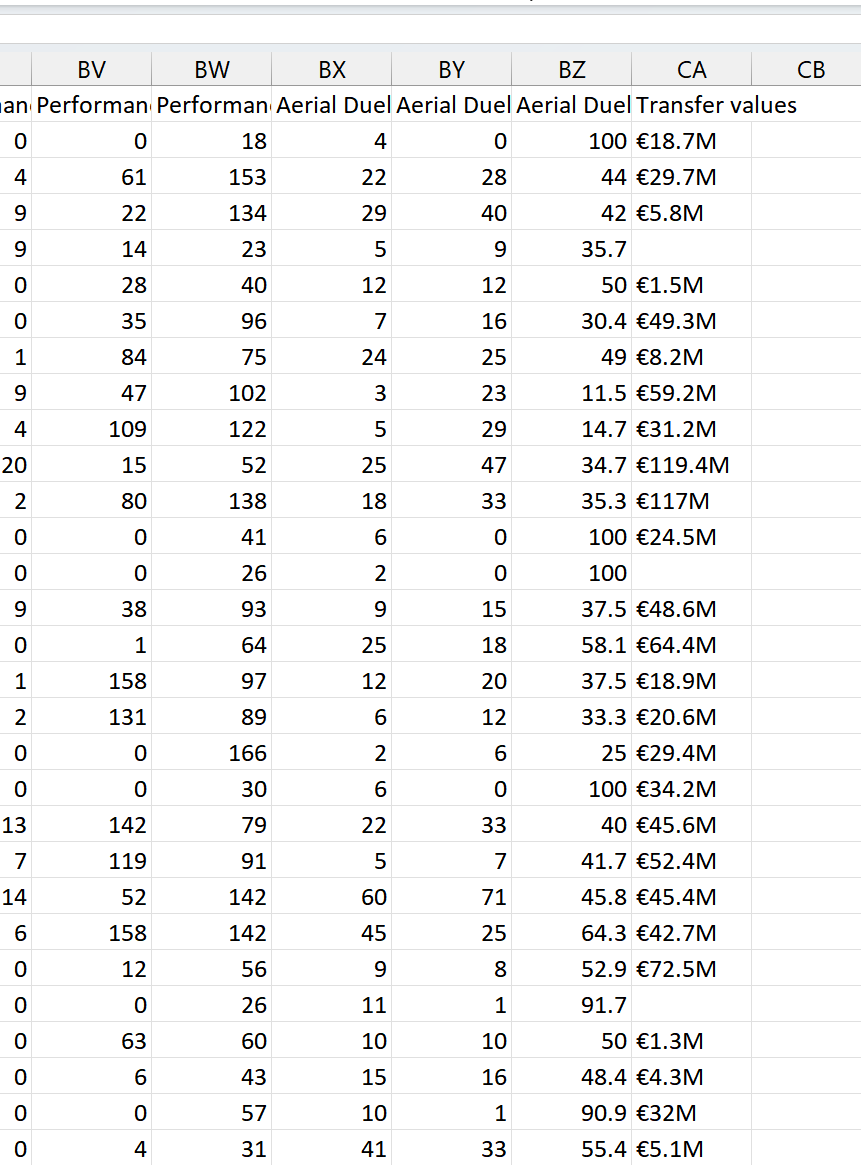
\includegraphics[width=300px]{P41_RES.png}
    \caption{File MoreThan900mins.csv}
    \label{fig:res2}
\end{figure}
File "MoreThan900mins.csv" là một tập dữ liệu chứa thông tin chi tiết về các cầu thủ bóng đá đã thi đấu ít nhất 900 phút trong mùa giải. Dữ liệu bao gồm 100 cầu thủ với 93 thuộc tính khác nhau, ghi lại các chỉ số liên quan đến hiệu suất thi đấu, thống kê cá nhân, và thông tin chung như tên, quốc tịch, đội bóng, vị trí, tuổi, giá trị chuyển nhượng, cùng các chỉ số chi tiết như thời gian thi đấu, số bàn thắng, kiến tạo, thẻ phạt, các chỉ số dự kiến (xG, xAG), và nhiều chỉ số khác liên quan đến khả năng chuyền bóng, phòng ngự, tấn công, và kiểm soát bóng.
\\
Dữ liệu được tổ chức theo định dạng CSV, với mỗi hàng đại diện cho một cầu thủ và mỗi cột là một thuộc tính cụ thể. Các thuộc tính bao gồm cả thông tin cơ bản (ví dụ: tên, đội bóng) và các chỉ số chuyên sâu. File này có thể được sử dụng để phân tích hiệu suất cầu thủ, so sánh giữa các vị trí, hoặc đánh giá tiềm năng trong các kịch bản chuyển nhượng.
\\
File này đã được mở rộng thêm cột Tranfer Values với đơn vị là triệu euro.
\clearpage
\subsubsection{Đánh giá}
Phần chính ảnh hưởng đến thời gian thực thi và sử dụng bộ nhớ trong các tác vụ đang hoạt động là hàm \texttt{update\_data}. Hàm này thực hiện việc crawl dữ liệu từ một trang web bằng cách sử dụng Selenium để điều khiển trình duyệt Chrome và BeautifulSoup để phân tích cú pháp HTML. Quá trình web scraping này về bản chất là tốn thời gian do các yếu tố như độ trễ mạng, thời gian tải trang, và thời gian xử lý của trình duyệt. Việc sử dụng \texttt{time.sleep(2)} trong vòng lặp thu thập dữ liệu cũng góp phần đáng kể vào tổng thời gian chạy, nhằm mục đích chờ đợi nội dung trang tải hoàn chỉnh hoặc để tránh bị chặn bởi server. Điều này làm tăng tính ổn định của quá trình crawl nhưng đồng thời kéo dài đáng kể thời gian thực thi. Về mặt bộ nhớ, việc khởi tạo và duy trì một phiên bản trình duyệt (Chrome) thông qua Selenium tiêu thụ một lượng bộ nhớ đáng kể. Tuy nhiên, các thao tác xử lý dữ liệu bằng BeautifulSoup và lưu trữ trong dictionary \texttt{player\_dic} có vẻ không gây áp lực lớn lên bộ nhớ đối với quy mô dữ liệu hiện tại, dựa trên kết quả sử dụng bộ nhớ được báo cáo trước đó.

Các hàm \texttt{get\_data} và \texttt{save\_result} sử dụng thư viện pandas để đọc, lọc và ghi dữ liệu vào file CSV. Các thao tác với pandas có thể tiêu tốn bộ nhớ, đặc biệt với các tập dữ liệu lớn. Tuy nhiên, trong trường hợp này, dựa trên lượng bộ nhớ đạt đỉnh được báo cáo từ terminal, có vẻ như quy mô dữ liệu đang được xử lý không quá lớn, do đó tác động của pandas lên việc sử dụng bộ nhớ là chấp nhận được.

Tóm lại, đối với phần code đang hoạt động (\texttt{Task\_1}), yếu tố chính chi phối thời gian chạy là quá trình web scraping trong hàm \texttt{update\_data} do sự phụ thuộc vào mạng, trình duyệt và việc chủ động tạm dừng (\texttt{time.sleep}). Việc sử dụng bộ nhớ chủ yếu liên quan đến phiên bản trình duyệt của Selenium và các cấu trúc dữ liệu tạm thời, nhưng nhìn chung có vẻ hiệu quả đối với quy mô dữ liệu hiện tại. Các phép đo thời gian và bộ nhớ sử dụng \texttt{time} và \texttt{tracemalloc} ở cuối script cung cấp dữ liệu định lượng hữu ích để theo dõi hiệu suất tổng thể của chương trình.

\section{Xử lý yêu cầu 2}
\subsection{Chọn model và feature để xử lý}
\subsubsection{Lựa chọn model}
Random Forest Regressor là một thuật toán học máy có giám sát thuộc lớp các phương pháp học tập tổ hợp (Ensemble Learning), được phát triển bởi Leo Breiman và Adele Cutler. Nó kế thừa và cải tiến kỹ thuật \textit{Bootstrap Aggregating (Bagging)}, chủ yếu nhằm mục đích cải thiện độ chính xác dự đoán và kiểm soát hiện tượng quá khớp (overfitting) thường gặp ở các mô hình cây quyết định đơn lẻ. Thuật toán này đặc biệt hiệu quả cho các bài toán hồi quy (\textit{regression}), nơi mục tiêu là dự đoán một giá trị đầu ra liên tục.\\
\textbf{Nền tảng: Bagging và Cây Quyết Định}
\textbf{Cây Quyết Định (Decision Tree)}: Là các mô hình cơ sở (\textit{base estimators}) trong Random Forest. Một cây quyết định hồi quy hoạt động bằng cách phân chia không gian đặc trưng (\textit{feature space}) thành các vùng hình chữ nhật nhỏ hơn thông qua một chuỗi các quy tắc chia dựa trên giá trị của các đặc trưng. Tại mỗi nút lá, giá trị dự đoán thường là trung bình của các giá trị mục tiêu của các mẫu huấn luyện thuộc về nút lá đó. Cây quyết định đơn lẻ có xu hướng bị phương sai cao (\textit{high variance}), rất nhạy cảm với những thay đổi nhỏ trong dữ liệu huấn luyện và dễ bị quá khớp.

\textbf*{Bagging (Bootstrap Aggregating)}: Là một kỹ thuật tổng quát trong học tập tổ hợp nhằm giảm phương sai của bộ ước lượng. Gồm hai bước chính:

\begin{itemize}
    \item \textbf{Bootstrap Sampling}: Tạo ra $B$ tập dữ liệu huấn luyện mới (các mẫu bootstrap) từ tập dữ liệu huấn luyện gốc bằng cách lấy mẫu ngẫu nhiên có hoàn lại. Mỗi mẫu bootstrap có thể chứa các bản sao của một số điểm dữ liệu và bỏ sót một số khác. Trung bình, khoảng 63.2\% điểm dữ liệu gốc sẽ có mặt trong một mẫu bootstrap cụ thể.
    \item \textbf{Aggregating}: Huấn luyện một bộ ước lượng cơ sở (ví dụ: một cây quyết định) trên mỗi mẫu bootstrap. Đối với bài toán hồi quy, dự đoán được lấy trung bình từ $B$ ước lượng cơ sở:
    \[
    \hat{f}_{\text{bagging}}(x) = \frac{1}{B} \sum_{b=1}^{B} \hat{f}_b(x)
    \]
    trong đó $\hat{f}_b(x)$ là dự đoán từ cây thứ $b$ được huấn luyện trên mẫu bootstrap thứ $b$.
\end{itemize}

\textbf*{Cải tiến cốt lõi: Random Subspace Method}
Random Forest cải tiến Bagging bằng cách thêm một lớp ngẫu nhiên hóa gọi là \textit{Random Subspace Method} (hay \textit{feature bagging}). Khi xây dựng mỗi cây trên một mẫu bootstrap $D_b$, tại mỗi nút cần phân chia, thuật toán chỉ chọn ngẫu nhiên một tập con gồm $m$ đặc trưng (với $m < p$). Việc tìm điểm chia tốt nhất chỉ được thực hiện trong số $m$ đặc trưng đã chọn.

\textbf{Tham số $m$}: Đây là siêu tham số quan trọng, thường được chọn là $m \approx \frac{p}{3}$ đối với bài toán hồi quy. Việc chọn $m$ nhỏ giúp giảm tương quan giữa các cây trong rừng.

\textbf{Lý do cần giảm tương quan}: Trong Bagging chuẩn, nếu tồn tại các đặc trưng mạnh, chúng có thể được chọn thường xuyên ở các cây khác nhau, gây ra sự tương quan. Việc giảm tương quan giữa các cây sẽ giúp giảm phương sai tổng thể của mô hình mà không làm tăng đáng kể độ chệch.

\textbf*{Thuật toán Random Forest Regressor}
Cho tập huấn luyện $D = \{(x_1, y_1), ..., (x_N, y_N)\}$, số lượng cây $B$, và số đặc trưng tại mỗi nút là $m$:

\begin{enumerate}
    \item \textbf{For} $b = 1$ to $B$:
    \begin{enumerate}
        \item Tạo mẫu bootstrap $D_b$ bằng cách lấy mẫu ngẫu nhiên có hoàn lại từ $D$.
        \item Xây dựng cây hồi quy $T_b$ trên $D_b$:
        \begin{itemize}
            \item Tại mỗi nút: chọn ngẫu nhiên $m$ đặc trưng từ $p$ đặc trưng có sẵn.
            \item Tìm điểm chia tốt nhất trong $m$ đặc trưng được chọn.
            \item Phân chia nút thành hai nút con.
        \end{itemize}
        \item Tiếp tục cho đến khi đạt điều kiện dừng (ví dụ: số lượng mẫu tối thiểu ở nút lá).
    \end{enumerate}
    \item \textbf{Output}: Tập hợp các cây $\{T_b\}_{b=1}^{B}$.
    \item \textbf{Dự đoán}: Với điểm mới $x$, dự đoán là:
    \[
    \hat{f}_{\text{RF}}(x) = \frac{1}{B} \sum_{b=1}^{B} T_b(x)
    \]
\end{enumerate}

\textbf*{Ưu điểm học thuật}
\begin{itemize}
    \item \textbf{Độ chính xác cao}: Hiệu suất tốt trên nhiều loại dữ liệu.
    \item \textbf{Chống quá khớp}: Giảm phương sai nhờ Bagging và random subspace.
    \item \textbf{Xử lý tốt dữ liệu chiều cao}: Hoạt động hiệu quả ngay cả khi $p > N$.
    \item \textbf{Ước lượng lỗi nội bộ (Out-of-Bag Error)}: Cho phép ước lượng lỗi mà không cần tập kiểm tra.
    \item \textbf{Đo lường tầm quan trọng đặc trưng}: Cho biết mức độ quan trọng của từng đặc trưng.
\end{itemize}

\textbf*{Nhược điểm học thuật}
\begin{itemize}
    \item \textbf{Tính diễn giải thấp}: Là mô hình "hộp đen".
    \item \textbf{Chi phí tính toán cao}: Cần nhiều tài nguyên, đặc biệt với $B$ lớn. Tuy nhiên, việc huấn luyện có thể song song hóa.
\end{itemize}

\textbf*{Lý do lựa chọn Model (RandomForestRegressor):}
\begin{itemize}
    \item \textbf{Bài toán hồi quy (Regression Task)}: Mục tiêu của bài toán là dự đoán một giá trị số liên tục (ví dụ: giá trị chuyển nhượng của cầu thủ), do đó cần áp dụng một mô hình hồi quy. Random Forest Regressor là một lựa chọn tự nhiên và hiệu quả trong ngữ cảnh này.
    
    \item \textbf{Khả năng xử lý quan hệ phi tuyến (Non-linearity)}: Mối quan hệ giữa các đặc trưng như tuổi, chỉ số kỹ thuật, và giá trị thị trường thường không tuyến tính. Ví dụ, giá trị cầu thủ có thể tăng theo tuổi khi còn trẻ, đạt đỉnh ở độ tuổi nhất định và sau đó giảm dần. Random Forest có khả năng mô hình hóa các quan hệ phi tuyến phức tạp này một cách hiệu quả.
    
    \item \textbf{Hiệu năng dự đoán tốt (Good Performance)}: Random Forest thường cho kết quả dự đoán chính xác trên nhiều loại tập dữ liệu khác nhau mà không yêu cầu quá nhiều tinh chỉnh tham số. Đây là một mô hình mạnh mẽ và đáng tin cậy cho nhiều bài toán thực tế.
    
    \item \textbf{Độ bền vững với ngoại lệ và không yêu cầu chuẩn hóa (Robustness)}: Mô hình Random Forest ít nhạy cảm với các giá trị ngoại lệ và không yêu cầu chuẩn hóa (scaling) các đặc trưng đầu vào. Điều này giúp đơn giản hóa quy trình tiền xử lý dữ liệu.
    
    \item \textbf{Khả năng xử lý đặc trưng phân loại (Categorical Feature Handling)}: Sau khi các đặc trưng phân loại được mã hóa (ví dụ bằng One-Hot Encoding), Random Forest có thể xử lý tốt và tận dụng được thông tin từ các đặc trưng này.
    
    \item \textbf{Ước lượng tầm quan trọng của đặc trưng (Feature Importance)}: Mô hình có khả năng đánh giá mức độ ảnh hưởng của từng đặc trưng đến kết quả dự đoán, từ đó cung cấp hiểu biết sâu hơn về các yếu tố quyết định giá trị cầu thủ.
    
    \item \textbf{Lựa chọn thay thế}: Mặc dù các mô hình khác như Gradient Boosting (XGBoost, LightGBM, CatBoost), Support Vector Regression (SVR), hoặc mạng nơ-ron (Neural Networks) cũng có thể được áp dụng, nhưng Random Forest là một lựa chọn khởi đầu vững chắc, dễ triển khai và phổ biến trong thực hành.
\end{itemize}
\subsubsection{Lựa chọn feature}
Không chỉ dừng lại ở việc phân tích những dữ liệu ở trong những dữ liệu thu thập được, để lựa chọn được những feature ảnh hưởng nhiều nhất, tác động lớn nhất tới giá cầu thủ cần tìm hiểu nghiên cứu nhiều nguồn tài liệu khác nhau. Đặc biệt là phải đi phân tích những bài báo khoa học bài nghiên cứu để chọn ra những feature tốt nhất. Qua quá trình nghiên cứu đã xác định được một số feature đặc trưng ảnh hưởng lớn đến giá trị chuyển nhượng của cầu thủ:
\begin{enumerate}
    \item \textbf{Age} (Tuổi): Đặc trưng dạng số liên tục (numerical). Tuổi tác thường ảnh hưởng phi tuyến đến giá trị cầu thủ, khi giá trị có thể đạt đỉnh ở độ tuổi nhất định và giảm dần sau đó.
    
    \item \textbf{Position} (Vị trí thi đấu): Đặc trưng phân loại (categorical) mô tả vai trò chiến thuật của cầu thủ trên sân (ví dụ: tiền đạo, hậu vệ, tiền vệ). Được chuyển đổi thành dạng số bằng kỹ thuật mã hóa One-Hot (OneHotEncoder) để phù hợp với mô hình học máy.
    
    \item \textbf{Playing Time: minutes} (Tổng số phút thi đấu): Đặc trưng dạng số liên tục, phản ánh mức độ được sử dụng của cầu thủ trong mùa giải – thường tương quan tích cực với giá trị thị trường.
    
    \item \textbf{Performance: goals} (Số bàn thắng): Đặc trưng dạng số biểu thị số lượng bàn thắng mà cầu thủ ghi được. Đây là chỉ số quan trọng, đặc biệt với các cầu thủ tấn công.
    
    \item \textbf{Performance: assists} (Số lần kiến tạo): Đặc trưng dạng số thể hiện khả năng hỗ trợ ghi bàn. Cùng với bàn thắng, đây là thước đo chính về hiệu quả đóng góp vào khâu tấn công.
    
    \item \textbf{GCA: GCA} (Goal-Creating Actions): Đặc trưng dạng số liên tục, biểu diễn số hành động trực tiếp dẫn đến bàn thắng (ví dụ: đường chuyền quyết định, rê bóng vượt qua đối thủ trước bàn thắng). Là chỉ số tổng hợp cho khả năng sáng tạo.
    
    \item \textbf{Progression: PrgR} (Progressive Receptions): Đặc trưng dạng số đo lường số lần cầu thủ nhận bóng ở các vị trí có giá trị tiến bộ (forward-moving). Thể hiện khả năng di chuyển và nhận bóng chiến thuật.
    
    \item \textbf{Tackles: Tkl} (Số lần tắc bóng thành công): Đặc trưng dạng số biểu diễn khả năng phòng ngự, đặc biệt quan trọng với các cầu thủ phòng ngự như hậu vệ hoặc tiền vệ phòng ngự.
\end{enumerate}
Tập đặc trưng này bao gồm cả thông tin định lượng và định tính, được chọn lọc để bao phủ nhiều khía cạnh trong lối chơi và hiệu suất thi đấu, từ tấn công, hỗ trợ đến phòng ngự.
Việc lựa chọn đặc trưng (feature selection) là một bước quan trọng trong quy trình xây dựng mô hình học máy, đặc biệt đối với các bài toán hồi quy trong bối cảnh dữ liệu thể thao. Các đặc trưng được lựa chọn trong mô hình có tính phù hợp cao dựa trên các tiêu chí sau:

\begin{itemize}
    \item \textbf{Liên quan (Relevance)}: Các đặc trưng được chọn đều là những chỉ số thống kê phổ biến và có cơ sở chuyên môn rõ ràng trong lĩnh vực bóng đá. Cụ thể, tuổi tác, vị trí thi đấu, thời gian thi đấu, khả năng ghi bàn và kiến tạo, chỉ số hỗ trợ tấn công (GCA, PrgR), cũng như chỉ số phòng ngự (Tkl) đều phản ánh trực tiếp đến hiệu suất thi đấu và từ đó ảnh hưởng đến giá trị thị trường của cầu thủ.
    
    \item \textbf{Tính sẵn có (Availability)}: Các đặc trưng này là dữ liệu được thu thập phổ biến và dễ tiếp cận, thường có trong các cơ sở dữ liệu bóng đá lớn như FBref, Opta hay StatsBomb. Điều này đảm bảo tính khả thi khi triển khai mô hình trong thực tế.
    
    \item \textbf{Đa dạng (Diversity)}: Bộ đặc trưng bao gồm thông tin đa chiều: thông tin cá nhân (tuổi, vị trí), thời gian thi đấu (minutes), khả năng tấn công (goals, assists, GCA, PrgR) và khả năng phòng ngự (Tkl). Điều này tạo ra một cái nhìn toàn diện về năng lực cầu thủ trên cả khía cạnh chiến thuật và thống kê.
    
    \item \textbf{Lưu ý trong thực hành (Practical Note)}: Việc lựa chọn đặc trưng không hoàn toàn mang tính cố định mà thường trải qua quá trình thử nghiệm và hiệu chỉnh. Ban đầu có thể dựa trên kiến thức chuyên môn, phân tích dữ liệu khám phá (exploratory data analysis), hoặc sử dụng các kỹ thuật tự động như \textit{Recursive Feature Elimination} hay \textit{feature importance} từ mô hình cây. Việc đánh giá hiệu quả của tập đặc trưng được thực hiện thông qua các chỉ số đánh giá mô hình như MAE, RMSE hoặc $R^2$.
\end{itemize}
\subsection{Code thực tế và mô tả}
\begin{lstlisting}
def estimate_player_value(file_path):
    # Load data
    df = pd.read_csv(file_path)
    
    # Clean minutes column if necessary
    if df['Playing Time: minutes'].dtype == object:
        df['Playing Time: minutes'] = df['Playing Time: minutes'].str.replace(',', '').astype(int)
    
    # Fix Transfer values format to int
    df = df.dropna(subset=['Transfer values'])
    df['Transfer values'] = df['Transfer values'].str.replace('€', '', regex=False).str.replace('M', '', regex=False).astype(float) * 1_000_000
    df['Transfer values'] = df['Transfer values'].astype(int)

    # Select features
    features = [
        'Age',
        'Position',
        'Playing Time: minutes',
        'Performance: goals',
        'Performance: assists',
        'GCA: GCA',
        'Progression: PrgR',
        'Tackles: Tkl'
    ]

    X = df[features]
    y = df['Transfer values']
    
    # Split data
    X_train, X_test, y_train, y_test = train_test_split(X, y, test_size=0.2, random_state=42)

    # Preprocessing: OneHot for categorical 'Position'
    categorical_features = ['Position']
    numeric_features = [col for col in features if col not in categorical_features]
    
    preprocessor = ColumnTransformer(
        transformers=[
            ('cat', OneHotEncoder(handle_unknown='ignore'), categorical_features)
        ],
        remainder='passthrough'  # Numeric features stay unchanged
    )
    
    # Model
    model = RandomForestRegressor(n_estimators=100, random_state=42)
    
    # Pipeline
    pipeline = Pipeline(steps=[
        ('preprocessor', preprocessor),
        ('model', model)
    ])
    
    # Train
    pipeline.fit(X_train, y_train)
    
    # Predict and evaluate
    y_pred = pipeline.predict(X_test)
    mae = mean_absolute_error(y_test, y_pred)
    print(f"Mean Absolute Error: {mae:,.0f} €")
    
    return pipeline
\end{lstlisting}
Hàm này thực hiện một quy trình xây dựng và đánh giá một mô hình học máy (Machine Learning) để ước tính giá trị chuyển nhượng (\textit{Transfer values}) của cầu thủ bóng đá dựa trên các số liệu thống kê của họ.

\textbf{Quy trình hoạt động}

\textbf{1. Tải dữ liệu (Load Data)}:
\begin{verbatim}
df = pd.read_csv(file_path)
\end{verbatim}
Hàm này đọc dữ liệu từ một file CSV (được chỉ định bởi \texttt{file\_path}) vào một cấu trúc dữ liệu dạng bảng gọi là DataFrame của thư viện pandas, đặt tên là \texttt{df}.

\textbf{2. Làm sạch dữ liệu (Clean Data)}:
\textbf{Xử lý cột 'Playing Time: minutes'}:
Kiểm tra kiểu dữ liệu của cột \texttt{'Playing Time: minutes'}, nếu kiểu là \texttt{'object'} (chuỗi), loại bỏ dấu phẩy và chuyển đổi kiểu dữ liệu thành số nguyên:
\begin{verbatim}
df['Playing Time: minutes'] = df['Playing Time: minutes'].str.replace(',', '').astype(int)
\end{verbatim}

\textbf{Xử lý cột 'Transfer values'}:
Loại bỏ các giá trị thiếu (\texttt{NaN}) và chuyển đổi giá trị chuyển nhượng từ chuỗi (ví dụ: "\€50.5M") sang số thực:
\begin{verbatim}
df = df.dropna(subset=['Transfer values'])
df['Transfer values'] = df['Transfer values'].str.replace('€', '', regex=False).str.replace('M', '', regex=False).astype(float) * 1_000_000
df['Transfer values'] = df['Transfer values'].astype(int)
\end{verbatim}

\textbf{3. Chọn Features (Đặc trưng - Biến đầu vào)}:
Chọn các đặc trưng có ảnh hưởng đến giá trị chuyển nhượng của cầu thủ:
\begin{verbatim}
features = ['Age', 'Position', 'Playing Time: minutes', 'Performance: goals', 'Performance: assists', 'GCA: GCA', 'Progression: PrgR', 'Tackles: Tkl']
X = df[features]
y = df['Transfer values']
\end{verbatim}

\textbf{4. Phân chia dữ liệu (Split Data)}:
Chia dữ liệu thành tập huấn luyện và tập kiểm tra với tỉ lệ 80/20:
\begin{verbatim}
from sklearn.model_selection import train_test_split
X_train, X_test, y_train, y_test = train_test_split(X, y, test_size=0.2, random_state=42)
\end{verbatim}

\textbf{5. Tiền xử lý dữ liệu (Preprocessing)}:
Xử lý các đặc trưng phân loại và số:
\begin{verbatim}
from sklearn.compose import ColumnTransformer
from sklearn.preprocessing import OneHotEncoder

categorical_features = ['Position']
numeric_features = ['Age', 'Playing Time: minutes', 'Performance: goals', 'Performance: assists', 'GCA: GCA', 'Progression: PrgR', 'Tackles: Tkl']

preprocessor = ColumnTransformer(
    transformers=[
        ('cat', OneHotEncoder(handle_unknown='ignore'), categorical_features),
        ('num', 'passthrough', numeric_features)
    ])
\end{verbatim}

\textbf{6. Chọn và Khởi tạo Model}:
Sử dụng mô hình \texttt{RandomForestRegressor} với 100 cây quyết định:
\begin{verbatim}
from sklearn.ensemble import RandomForestRegressor
model = RandomForestRegressor(n_estimators=100, random_state=42)
\end{verbatim}

\textbf{7. Tạo Pipeline}:
Kết hợp các bước tiền xử lý và mô hình vào một Pipeline:
\begin{verbatim}
from sklearn.pipeline import Pipeline
pipeline = Pipeline(steps=[
    ('preprocessor', preprocessor),
    ('model', model)
])
\end{verbatim}

\textbf{8. Huấn luyện mô hình (Train)}:
Huấn luyện mô hình với dữ liệu huấn luyện:
\begin{verbatim}
pipeline.fit(X_train, y_train)
\end{verbatim}

\textbf{9. Dự đoán và Đánh giá (Predict and Evaluate)}:
Dự đoán giá trị chuyển nhượng và đánh giá mô hình bằng sai số tuyệt đối trung bình (MAE):
\begin{verbatim}
from sklearn.metrics import mean_absolute_error
y_pred = pipeline.predict(X_test)
mae = mean_absolute_error(y_test, y_pred)
print(f"Mean Absolute Error: {mae:,.0f} €")
\end{verbatim}

\textbf{10. Trả về kết quả}:
Trả về mô hình đã huấn luyện:
\begin{verbatim}
return pipeline
\end{verbatim}

\subsection{Kiểm thử và đánh giá}
\textbf{Kiểm thử}\\
\begin{lstlisting}
def Task_2():
    # Example usage
    model = estimate_player_value('MoreThan900mins.csv')

    new_player = pd.DataFrame({
        'Age': [26],
        'Position': ['GK'],
        'Playing Time: minutes': [2250],
        'Performance: goals': [0],
        'Performance: assists': [0],
        'GCA: GCA': [0],
        'Progression: PrgR': [0],
        'Tackles: Tkl': [0]
    })

    # Dự đoán giá trị cầu thủ mới
    predicted_value = model.predict(new_player)
    print(f"Estimated player value: {predicted_value[0]:,.0f} €")
\end{lstlisting}
chỉ số dòng và sử dụng mã hóa \texttt{'utf-8-sig'} để đảm bảo khả năng đọc file tốt hơn (dòng 3).

\begin{figure}[h]
    \centering
    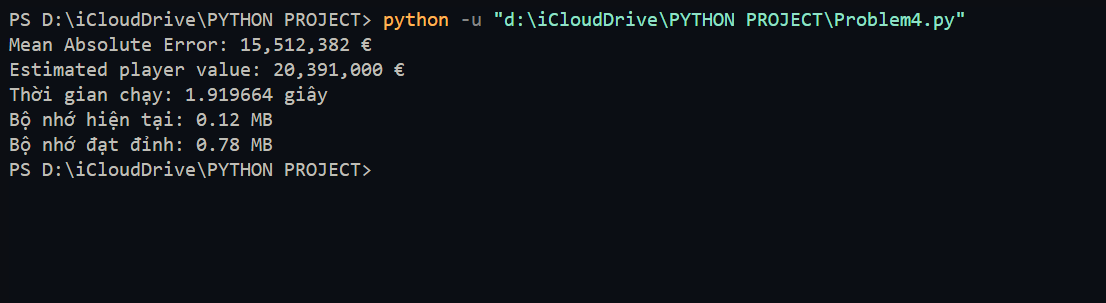
\includegraphics[width=300px]{Terminal_41.png}
    \caption{Terminal sau khi thực hiện function Task\_2}
    \label{fig:res4}
\end{figure}
Kết quả cho thấy thời gian hoàn thành là khoảng 1.92 giây và lượng bộ nhớ tiêu thụ đạt đỉnh ở mức 0.78 MB, cùng với các kết quả tính toán cụ thể như Mean Absolute Error và Estimated player value.

Từ góc độ học thuật, môi trường thực thi được trình bày thông qua giao diện dòng lệnh tiêu chuẩn với tông màu tối. Phân tích kết quả cho thấy script Python đạt hiệu năng thời gian xấp xỉ 1.92 giây và hiệu quả sử dụng bộ nhớ đáng chú ý khi chỉ yêu cầu tối đa 0.78 MB, cung cấp dữ liệu thực nghiệm quan trọng để đánh giá và tối ưu hóa hiệu suất tài nguyên của chương trình.

\textbf{Đánh giá}\\
Phân tích mã nguồn \texttt{Problem4.py} và kết quả thực thi cho thấy chương trình tập trung vào việc xây dựng một mô hình học máy dự đoán giá trị cầu thủ dựa trên các đặc trưng thống kê. Các phần hoạt động ổn định và hiệu quả bao gồm quy trình xử lý dữ liệu ban đầu (tải, làm sạch cơ bản các cột số), lựa chọn đặc trưng, chia tách tập dữ liệu, và đặc biệt là việc triển khai pipeline học máy sử dụng \texttt{scikit-learn}. Pipeline này kết hợp tiền xử lý dữ liệu phân loại bằng One-Hot Encoding thông qua \texttt{ColumnTransformer} và mô hình hồi quy \texttt{Random Forest}. 

Kết quả thực thi từ terminal xác nhận tính năng động của pipeline này, hiển thị Lỗi tuyệt đối trung bình (Mean Absolute Error - MAE) là \textbf{15.512.382 €}, một chỉ số định lượng về độ chính xác của mô hình trên tập dữ liệu kiểm tra. Giá trị cầu thủ ước tính cho một trường hợp cụ thể là \textbf{20.391.000 €}. Chương trình cũng tích hợp chức năng đo lường hiệu năng, ghi nhận thời gian chạy là khoảng \textbf{1.92 giây} và mức sử dụng bộ nhớ đạt đỉnh là \textbf{0.78 MB}, cho thấy hiệu quả tương đối về tài nguyên đối với quy mô dữ liệu được xử lý trong lần chạy này.

\textbf{Ưu điểm của mã nguồn:}
\begin{itemize}
    \item \textbf{Tính mô-đun}: Mã được tổ chức thành các hàm riêng biệt cho từng tác vụ (lấy dữ liệu, cập nhật dữ liệu, lưu kết quả, xây dựng mô hình, các task cụ thể), giúp tăng khả năng đọc và bảo trì.
    \item \textbf{Sử dụng thư viện chuẩn mạnh mẽ}: Tận dụng hiệu quả các thư viện phổ biến và tối ưu hóa cao như \texttt{pandas} cho xử lý dữ liệu, \texttt{scikit-learn} cho học máy (bao gồm \texttt{Pipeline}, \texttt{ColumnTransformer}, \texttt{RandomForestRegressor}), và \texttt{time}/\texttt{tracemalloc} cho phân tích hiệu năng.
    \item \textbf{Triển khai Pipeline học máy}: Việc sử dụng Pipeline và ColumnTransformer là phương pháp tốt để xử lý các bước tiền xử lý và mô hình hóa một cách có hệ thống, giúp tránh rò rỉ dữ liệu (data leakage) giữa các bước, đặc biệt quan trọng trong quá trình đánh giá mô hình.
    \item \textbf{Đo lường hiệu năng tích hợp}: Việc thêm các đoạn mã đo thời gian chạy và bộ nhớ sử dụng là một điểm cộng lớn, cung cấp thông tin cần thiết để đánh giá và tối ưu hóa hiệu quả tài nguyên của chương trình.
\end{itemize}

\textbf{Nhược điểm của mã nguồn:}
\begin{itemize}
    \item \textbf{Độ chính xác}: Chỉ số MAE là \textbf{15.512.382 €} là một con số cụ thể, nhưng việc đánh giá "độ chính xác cao" hay thấp phụ thuộc vào bối cảnh của bài toán (phạm vi giá trị chuyển nhượng, tính biến động của dữ liệu, so sánh với các mô hình khác hoặc baseline). Nếu không có thêm thông tin so sánh, khó có thể kết luận về tính hiệu quả thực sự của mô hình.
    \item \textbf{Phụ thuộc vào nguồn dữ liệu ngoại vi}: Hàm \texttt{update\_data} phụ thuộc mạnh mẽ vào cấu trúc HTML của website \texttt{footballtransfers.com}. Bất kỳ thay đổi nào trên website đều có thể làm hỏng chức năng crawl dữ liệu, khiến phần này trở nên kém bền vững.
    \item \textbf{Thiếu xử lý lỗi mạnh mẽ}: Mặc dù có xử lý \texttt{try...except} cơ bản trong phần crawl, mã chưa có cơ chế xử lý lỗi toàn diện hơn cho các trường hợp như tệp dữ liệu đầu vào không tồn tại, định dạng dữ liệu không đúng, hoặc lỗi kết nối khi crawl.
    \item \textbf{Thiếu tùy chỉnh và đánh giá mô hình sâu hơn}: Mã chỉ sử dụng một loại mô hình (\texttt{RandomForestRegressor}) với các tham số mặc định (\texttt{n\_estimators=100}) và chỉ đánh giá trên một lần chia tách dữ liệu (\texttt{test\_size=0.2}). Việc khám phá các mô hình khác, điều chỉnh siêu tham số (hyperparameter tuning), và sử dụng Cross-validation sẽ cung cấp đánh giá độ tin cậy và tiềm năng cải thiện hiệu suất mô hình tốt hơn.
    \item \textbf{Đường dẫn tệp cố định}: Các đường dẫn tệp đầu vào và đầu ra được mã hóa cứng, làm giảm tính linh hoạt và khả năng tái sử dụng của mã trên các hệ thống hoặc cấu trúc thư mục khác nhau.
\end{itemize}

\textbf{Tóm lại}, mã nguồn thể hiện sự hiểu biết về quy trình xử lý dữ liệu và xây dựng mô hình học máy bằng các thư viện chuẩn. Các phần cốt lõi liên quan đến ML pipeline và đo lường hiệu năng hoạt động tốt. Tuy nhiên, tính phụ thuộc vào nguồn dữ liệu ngoại vi không ổn định, sự thiếu vắng xử lý lỗi toàn diện và việc đánh giá mô hình chưa chuyên sâu là những điểm có thể cải thiện.
}

\chapter*{Kết luận}
{
\noindent
Báo cáo này đã trình bày quá trình thực hiện một loạt các nhiệm vụ phân tích dữ liệu bóng đá sử dụng ngôn ngữ lập trình Python, tập trung vào việc thu thập, xử lý, phân tích và mô hình hóa dữ liệu thống kê cầu thủ từ giải Ngoại hạng Anh mùa giải 2004--2005 và dữ liệu chuyển nhượng gần đây.

\vspace{1em}
\noindent
\textbf{Tóm tắt kết quả chính:}

\vspace{0.5em}
\noindent
\textit{Thu thập và Tiền xử lý Dữ liệu (Vấn đề I):} Đã thành công trong việc thu thập dữ liệu thống kê chi tiết cho 491 cầu thủ thi đấu trên 90 phút từ trang \texttt{fbref.com} bằng kỹ thuật web scraping với Selenium và BeautifulSoup. Dữ liệu được làm sạch, chuẩn hóa (các giá trị không có sẵn được đánh dấu ``N/a'') và lưu trữ có cấu trúc trong tệp \texttt{results.csv}. Quá trình này đảm bảo tính chính xác và đầy đủ của dữ liệu nhưng cho thấy hiệu suất thời gian chưa tối ưu (\textasciitilde186 giây) do việc khởi tạo nhiều trình duyệt. Tuy nhiên, việc sử dụng bộ nhớ lại khá hiệu quả (\textasciitilde32.74 MB).

\vspace{0.5em}
\noindent
\textit{Phân tích Thống kê Mô tả (Vấn đề II):} Đã tiến hành phân tích sâu hơn trên tệp \texttt{results.csv}. Xác định được top 3 cầu thủ có chỉ số cao nhất và thấp nhất cho từng thống kê (lưu tại \texttt{top\_3.txt}). Tính toán các đại lượng thống kê mô tả quan trọng (trung vị, trung bình, độ lệch chuẩn) cho toàn giải đấu và từng đội (lưu tại \texttt{results2.csv}). Trực quan hóa sự phân phối của các chỉ số chính thông qua biểu đồ histogram (lưu dưới dạng file PNG). Dựa trên số lượng chỉ số dẫn đầu, Liverpool được xác định là đội có hiệu suất tổng thể tốt nhất (dẫn đầu 28 chỉ số, kết quả lưu tại \texttt{best\_team\_summary.txt}). Phân tích này cung cấp cái nhìn đa chiều về hiệu suất cầu thủ và đội bóng, dù phương pháp xác định đội tốt nhất còn tương đối đơn giản.

\vspace{0.5em}
\noindent
\textit{Phân cụm Cầu thủ (Vấn đề III):} Áp dụng thuật toán K-means để phân nhóm cầu thủ dựa trên dữ liệu thống kê. Số cụm tối ưu được xác định là $K=6$ thông qua phương pháp Elbow và Silhouette Score, phù hợp với các nhóm vị trí thực tế trong bóng đá. Kỹ thuật PCA được sử dụng để giảm chiều dữ liệu xuống 2 chiều, cho phép trực quan hóa các cụm cầu thủ một cách hiệu quả. Phân tích đặc điểm của từng cụm cho thấy sự tương đồng về vai trò hoặc phong cách chơi của các cầu thủ trong cùng một nhóm (kết quả phân tích và biểu đồ lưu trong thư mục \texttt{P3\_RES}). Mặc dù K-means và PCA có những hạn chế nhất định (giả định về hình dạng cụm, mất mát thông tin), phương pháp này đã cung cấp những hiểu biết ban đầu hữu ích về cấu trúc tiềm ẩn trong dữ liệu cầu thủ.

\vspace{0.5em}
\noindent
\textit{Ước tính Giá trị Cầu thủ (Vấn đề IV):} Đã thu thập dữ liệu giá trị chuyển nhượng từ \texttt{footballtransfers.com} cho các cầu thủ thi đấu trên 900 phút (lưu tại \texttt{MoreThan900mins.csv}). Đề xuất và triển khai thành công mô hình \texttt{RandomForestRegressor} để ước tính giá trị cầu thủ. Các đặc trưng đầu vào quan trọng như Tuổi, Vị trí, Thời gian thi đấu, Bàn thắng, Kiến tạo, GCA, PrgR, Tkl đã được lựa chọn dựa trên kiến thức chuyên môn và nghiên cứu. Mô hình đạt được Sai số Tuyệt đối Trung bình (MAE) khoảng €15.5 triệu trên tập kiểm tra. Việc sử dụng \texttt{Pipeline} trong Scikit-learn giúp quy trình tiền xử lý và huấn luyện được thực hiện một cách có hệ thống. Tuy nhiên, mô hình còn phụ thuộc vào nguồn dữ liệu bên ngoài và cần cải thiện về độ chính xác cũng như đánh giá sâu hơn (ví dụ: tinh chỉnh siêu tham số, sử dụng cross-validation).

\vspace{1em}
\noindent
\textbf{Đánh giá chung:}

\vspace{0.5em}
\noindent
Tổng thể, dự án đã hoàn thành tốt các mục tiêu đề ra, thể hiện được năng lực áp dụng các kỹ thuật khoa học dữ liệu từ thu thập, xử lý, phân tích đến mô hình hóa trong lĩnh vực thể thao. Việc sử dụng hiệu quả các thư viện Python như \texttt{Pandas}, \texttt{Scikit-learn}, \texttt{Selenium}, \texttt{BeautifulSoup} là một điểm mạnh nổi bật. Các kết quả phân tích và mô hình hóa cung cấp những thông tin giá trị về hiệu suất cầu thủ, đặc điểm đội bóng và các yếu tố ảnh hưởng đến giá trị chuyển nhượng.

\vspace{0.5em}
\noindent
Tuy nhiên, vẫn còn một số điểm có thể cải thiện như tối ưu hóa tốc độ web scraping, xây dựng các chỉ số đánh giá tổng hợp phức tạp hơn, và thực hiện đánh giá mô hình một cách toàn diện hơn. Sự phụ thuộc vào cấu trúc các trang web bên ngoài cũng là một yếu điểm cần lưu ý về tính bền vững của giải pháp thu thập dữ liệu.

\vspace{0.5em}
\noindent
Nhìn chung, báo cáo này là một minh chứng cho khả năng ứng dụng mạnh mẽ của Python và các kỹ thuật học máy trong việc khám phá và rút ra tri thức từ dữ liệu bóng đá phức tạp.

}

\chapter*{Danh mục tài liệu tham khảo}
{
\begin{enumerate}
    \item Scikit-learn Developers. (n.d.). RandomForestRegressor. Scikit-learn documentation.
    \item GeeksforGeeks. (n.d.). Random Forest Regression in Python.
    \item Université du Luxembourg. (2020). Random Forest Regression [Project Report].
    \item StatQuest with Josh Starmer. (n.d.). Random Forests Part 1: Regression [Video]. YouTube.
    \item Metelski, Adam. (2021). Factors affecting the value of football players in the transfer market. Journal of Physical Education and Sport. 21. 1150-1155. 10.7752/jpes.2021.s2145. 
    \item Rong, Zhangyi, Wang, Lujie, \& Xie, Shengting. (2024). \textit{Factors that Influence Player Market Value in Different Position: Evidence from European Leagues}. Advances in Economics, Management and Political Sciences, 82, 50--63.
    \item Football Benchmark. (n.d.). Game changers: A snapshot of the top 100 most valuable players. Football Benchmark.
    \item Zhang, Y., \& Zhang, W. (2019). \textit{Research on player value evaluation model based on multiple linear regression analysis}.
    \item Krabbenborg, L. (2020). The relationship between player market value and performance in professional European football: A statistical analysis (Bachelor's thesis, Tilburg University).

\end{enumerate}
}
\end{document}
